\documentclass[UTF8,fontset=none,11pt]{ctexart}
\usepackage[a4paper,margin=28mm]{geometry}
\usepackage{amsmath,amssymb,amsthm,mathtools}
\setCJKmainfont[ItalicFont={Noto Serif CJK SC},SlantedFont={Noto Serif CJK SC}]{Noto Serif CJK SC}
\setCJKsansfont{Noto Sans CJK SC}
\setCJKmonofont{Noto Sans Mono CJK SC}
\usepackage{tikz}
\usetikzlibrary{decorations.pathreplacing}
\usepackage[hidelinks]{hyperref}
\usepackage{xurl}
\hypersetup{pdftitle={星形Kakeya集的面积下界与重构障碍},pdfsubject={完整单位针、十分之一下界、上界构造与全类比较}}
\newtheoremstyle{zhplain}{7pt}{7pt}{\normalfont}{}{\bfseries}{.}{.5em}{}
\theoremstyle{zhplain}
\newtheorem{theorem}{定理}[section]
\newtheorem{lemma}[theorem]{引理}
\newtheorem{proposition}[theorem]{命题}
\newtheorem{corollary}[theorem]{推论}
\theoremstyle{definition}
\newtheorem{definition}[theorem]{定义}
\newtheorem{remark}[theorem]{说明}
\renewcommand{\proofname}{证明}
\numberwithin{equation}{section}
\numberwithin{figure}{section}
\title{星形 Kakeya 集的面积下界与重构障碍}
\author{}
\date{收尾研究稿}
\begin{document}
\maketitle
% 完整英文前言 intro_en.tex 的中文初译；待同底本精修。
\begin{abstract}
若平面星形集在每个无向方向上都包含一条闭单位线段，其 Lebesgue 外测度至少为 $1/10$。本文给出完整证明，不要求原集合可测、有界，也不假设能够规则地选择其中的针。证明测量实际的圆周截面，仅在近端点半径允许时使用第二个端点，并在同一份实际面积预算上平衡其余方向。随后，我们研究完整单位针的上界构造及其严格改进，再考察极值问题中若干重构方法的障碍。我们构造了一个固定的有限竞争星体 $K$：对每个同中心且容纳随方向连续、首尾闭合的单位针选择的紧星体 $Q$，都有 $|Q\setminus K|\ge\varepsilon_K>0$，而 $Q$ 的外半径可以任意大。一个规定的双剪切规则，也会在趋近面积下确界的有限输入上严格增加面积。有限采样、半径截断、最长完整弦及强面积闭合，进一步说明这些方法保留了什么信息。锐下确界仍未确定；缺少的比较必须把完整针的可行性与高效构造中的重叠关系结合起来。
\end{abstract}

\section{同一个中心与独立放置的针}\label{sec:introduction}
平面 Kakeya 条件要求每个方向上都有一条单位线段。不加其他几何要求时，这与任意小的面积相容。星形性增加了一项要求：必须存在一个点，使它与集合中每一点之间的线段都仍在该集合中。因此，每条可用的针都会带来径向材料。问题在于，独立放置这些针时，材料究竟能够重叠到什么程度。

Cunningham 在对星形 Kakeya 集的研究中证明了正的面积下界 $\pi/108$~\cite{Cunningham1971}。他在第 129 页的文末说明中指出，这个下界证明只使用每个方向存在一条单位线段，并未使用连续反转过程。Li 随后通过圆周截面估计，将这一静态问题的外测度下界提高到 $\pi/98$~\cite[定理~1.1]{Li2026}。本文沿用对实际圆周截面进行估计的思路，在内圆盘中进一步结合近端点资格与互补权重。连续闭合的针选择会另行明确引入，而不会作为任意 Kakeya 集的默认条件。

我们的第一个结果是
\[
 E\subset\mathbb R^2\text{ 为星形集且每个方向都有完整单位针}
 \quad\Longrightarrow\quad |E|^*\ge\frac1{10}.
\]
这里 $|E|^*$ 是 Lebesgue 外测度，星形中心可以是任意点。原针的选择可以完全不规则。转到任意开超集后，可以在该开集中重新选出可测族，再对实际的极坐标截面积分。所用的可测投影事实属于标准描述测度论~\cite{Kechris1995}；几何估计及完整的面积分配都在下文证明。

证明的低半径部分有一项具体的补偿关系。近端点离中心足够远的方向，提供两个不同的理想角度锚点；缺少第二个锚点的方向，则有半径更大的远端点，能在稍后的径向区间上给出更强的下界。对这两条估计作凸组合，可以让每个实际点至多贡献一次，并使最终的下界系数不依赖于两类方向各占多少。其余更大的端点尺度由互不相交的外侧径向区域处理。整个过程保留了零高度、垂足在底边外的情况、闭端点，以及实际角度与无向方向的区别。

上界构造从另一侧使用相同的几何对象。它们安排完整底边，使一个端点新增的材料被已有材料遮住，再利用仍然暴露的部分证明严格改进。这些改进必须在微观极限和有限记录恢复两步之后仍保持为正。因此，最后的伸长操作在原微观尺度下控制法向位移，并检查整条内接弦。它的比较适用于指定的源族，而不直接适用于任意近极小输入。

论文的其余部分考察哪些方法可以把这些构造传递到全体输入。两种方法因不同的几何原因失效：几乎保留一个固定星体的全部材料，可能与连续针选择不相容；固定剪切规则的闭轴分支，则可以积累出真正的新增面积。对空间逃逸和极限代表，则能给出正面结论。远处的针允许带有定量误差的半径截断；强面积度量允许构造实际的全方向代表，并给出全局相对替换不等式。这两项结果都尚未提供近极小序列的紧性或所缺少的锐值比较。区分它们的作用，才能明确后续论证需要增加什么。

\tableofcontents
\clearpage
% 中文精修稿；底本为 core_zh_initial.tex，英文快照为 core_translation_source.tex。
% 主文件提供中文排版支持、amsmath、amssymb、amsthm 及 theorem/lemma/proof 环境。
% 翻译与精修记录见 core_zh_sentence_audit.md；本文仍处于独立核验前的草稿阶段。

\section{星形 Kakeya 集的十分之一面积下界}
\label{sec:core-tenth}

% [E01]
星形集包含一条单位线段，就必然包含相应的三角形。把星形中心放在原点，取端点为 $(-1/2,h)$ 和 $(1/2,h)$ 的水平线段。原点与这条底边上任一点之间的线段都属于该集合，因此整个三角形都属于它。三角形的面积是 $|h|/2$。底边到原点的距离只要至少为 $1/5$，就得到了所求下界。

% [E02]
困难出现在每条选定的底边都靠近原点的情形。若 $h\ne0$，以原点为中心旋转整条底边及其三角形，就得到另一个同面积的三角形；底边的中点也随之转动。两者的内部会重叠：第一个三角形的内点在充分小的旋转之后仍然是内点。直接相加两个三角形的面积，会把重叠部分计算两次。另一种极端情形是 $h=0$：若取以原点为中点的线段的所有旋转，每个三角形的面积都为零，并集却是半径为 $1/2$ 的圆盘。这两个例子都要求我们测量并集本身。我们沿同心圆测量这个并集；每个三角形的截面至多由两个实际角度区间组成。

\begin{theorem}
\label{thm:core-tenth}
设 $E\subseteq\mathbb R^2$，且存在一点 $o\in\mathbb R^2$，使得对每个 $x\in E$ 都有 $[o,x]\subseteq E$。再设每个无向方向 $q\in\mathbb {RP}^1$ 上都有一条沿方向 $q$、长为一的闭线段包含在 $E$ 中。那么 $E$ 的 Lebesgue 外测度满足
\[
                 |E|^*\geq\frac1{10}.
\]
\end{theorem}

% [E03]
这个命题适用于平面的任意子集和任意星形中心。因此，证明必须自行构造可测对象，不能假设能从 $E$ 中可测地选出各方向的线段。得到可测族后，只要近端点离中心足够远，主要的几何估计就同时使用两个端点。近端点半径较小的方向则有半径更大的远端点，可以在更大的半径上补足贡献。我们在半径为 $1/2$ 的圆盘内平衡这两种贡献，再用互不相交的圆环处理其余方向。

\subsection{在开覆盖内重新选取可测三角形族}
\label{subsec:core-recovery}

% [R01]
把 $o$ 平移到 $0$，并任取一个开集 $G\supseteq E$。只需对每个这样的 $G$ 证明 $|G|\geq1/10$，因为 Lebesgue 外测度等于所有开超集测度的下确界。对每个方向 $q$，从 $E$ 中选出一条单位线段，记其端点为 $A_q,B_q$，并令
\[
                  T_q=\operatorname{conv}\{0,A_q,B_q\}.
\]
$T_q$ 中的每一点都位于 $0$ 与 $[A_q,B_q]$ 上某一点之间的线段上，所以 $T_q\subseteq E\subseteq G$。

% [R02]
暂时允许这些选择任意依赖于 $q$。这里采用与开头整体旋转不同的操作：固定一个选定三角形的底边中点，仅改变底边方向。不区分端点次序时，线段及三角形都随方向在 Hausdorff 距离下连续变化。这里的 Hausdorff 连续性指双向的逐点接近。对两次放置中用同一局部角度坐标匹配的端点，保持凸组合系数不变，所得三角形点的位移至多为两个端点位移的最大值；反向匹配也有同一估计。原三角形是开集 $G$ 内的紧集，因此充分小的变化仍留在 $G$ 中。于是，同一个中点在原方向的一个开邻域内都可使用。这些邻域覆盖紧圆周 $\mathbb {RP}^1$；从中取有限子覆盖 $O_1,\ldots,O_k$，相应中点记为 $c_1,\ldots,c_k$。

% [R03]
将 $q$ 分配给第一个包含它的 $O_j$，并用 $c_j$ 作为相应线段的中点。各集合 $O_j\setminus\bigcup_{i<j}O_i$ 都是 Borel 集，因此这给出了一个 Borel 中点选择。方向仍遍历整个射影圆周；有限的只是中点取值的列表。每个新三角形都包含在 $G$ 内，但它的底边未必属于原集合 $E$。以下用 $A_q,B_q,T_q$ 表示重新选出的对象。

% [R04]
下文需要一个可测性事实。完备可分度量空间中 Borel 子集的 Borel 像称为解析集。在本文的欧氏空间和角度空间中，解析集以及 Borel 集的投影都是 Lebesgue 可测的。这是本证明所需的可测投影定理。对一个 Borel 方向集 $V$，令
\begin{align*}
 W(V)&=\bigcup_{q\in V}T_q,\qquad W=W(\mathbb {RP}^1),\\
 S_r(V)&=\{\theta\in\mathbb R/(2\pi\mathbb Z):
                  r(\cos\theta,\sin\theta)\in W(V)\},\quad r>0.
\end{align*}
取 $q\in[0,\pi)$ 作为无向方向的实角度代表，固定 $u_q=(\cos q,\sin q)$ 和逆时针法向 $n_q=(-\sin q,\cos q)$。已选中点 $c(q)$ 是 Borel 映射，所以明确规定 $A_q=c(q)-u_q/2$、$B_q=c(q)+u_q/2$ 就得到两个 Borel 端点映射。映射
\[
 (q,a,b)\longmapsto aA_q+bB_q,
 \qquad a,b\geq0,\quad a+b\leq1,
\]
是 Borel 映射，在 $q\in V$ 时的像恰为 $W(V)$，故 $W(V)$ 是解析集。它的联合极坐标关联集
\[
 \{(r,\theta):r>0,\ r(\cos\theta,\sin\theta)\in W(V)\}
\]
也是解析集：在上式的等式中引入 $q,a,b$，再将所得 Borel 集投影即可。固定 $r$ 后用同样的论证，可知每个 $S_r(V)$ 都可测。因此，可以对实际并集使用极坐标积分与 Tonelli 定理，证明中所用的所有子族也都如此。
下文所说的 Borel 族，是指在一个 Borel 方向集上每个方向恰有一条单位线段，且端点映射为 Borel 映射；子族通过限制这些相同的映射得到。

% [R05]
在正交单位坐标下，将重新选出的线段写成
\[
 A=(s-1/2)u+h n,\qquad B=(s+1/2)u+h n,
\]
其中 $u$ 是其方向的 Borel 单位代表，$n$ 是将其旋转四分之一周所得的向量。若重新选出的任意一条线段满足 $|h|\geq1/5$，其三角形就包含于 $G$ 且面积至少为 $1/10$。因此，以下可对重新选出的族假设
\begin{equation}
                    |h(q)|<1/5\quad\hbox{对每个 }q.
\label{eq:core-height}
\end{equation}
这个分情形步骤必须放在重新选取之后。固定中点 $c_j$ 时，它的位置和范数不变，但相对于底边法向的分量 $h(q)=c_j\cdot n_q$ 可能随方向改变。

\subsection{实际角度、并集与单侧延伸估计}
\label{subsec:core-intervals}

% [I01]
无向方向组成一个长度为 $\pi$ 的圆周，实际角度则组成一个长度为 $2\pi$ 的圆周。两者都使用通常的长度测度，方向长度记为 $|V|$，实际角度长度记为 $|S|$。从实际角度到方向的映射将对径点认作同一点。对每个 $q\in V$，以 Borel 方式从它的两个提升中选择一个，所得角度集的长度是 $|V|$，而非 $2|V|$。具体地，以角度模 $\pi$ 表示无向方向，在坐标区间 $[0,\pi)$ 上用 Borel 函数 $\chi:V\to\{0,1\}$ 记录所选的一侧，提升就是 $q\mapsto q+\pi\chi(q)$。$\chi=0$ 和 $\chi=1$ 两部分的像落在不同的半圆上，后者只是平移 $\pi$，故两像的长度之和恰为 $|V|$。

% [I02]
区分这两个圆周后，就可以比较理想方向和实际圆弧。从原点看去，底边端点所在的方向未必就是底边自身的方向。我们把端点的实际角度区间延伸到这个理想方向，并控制整个并集增加的长度。下面的初等估计允许任意重叠、重复区间，以及向任一侧延伸。

\begin{lemma}[并集的单侧延伸]
\label{lem:core-interval}
设 $(J_i)_{i\in I}$ 是任意一族闭圆周区间，允许单点区间。固定 $\rho\geq0$，将每个 $J_i$ 的一端延长至多 $\rho|J_i|$，得到 $K_i$。则
\begin{equation}
 \left|\bigcup_{i\in I}K_i\right|^*
       \leq(1+2\rho)\left|\bigcup_{i\in I}J_i\right|^*.
\label{eq:core-interval}
\end{equation}
\end{lemma}

\begin{proof}
% [I03]
取包含 $\bigcup_iJ_i$ 的开圆周集 $O$。若 $O$ 是整个圆周，它的测度已经给出了延伸后并集所需的上界。否则，$O$ 是可数个互不相交开弧的并。由于 $J_i$ 连通，它必包含在某个长为 $\ell$ 的连通分支 $C$ 中，且 $|J_i|\leq\ell$。将 $C$ 的两端各延伸 $\rho\ell$，就包含了所有对应的 $K_i$；即使延伸后绕过整圈，其圆周长度也至多为 $(1+2\rho)\ell$。这些扩大的分支覆盖延伸后的并集。先用测度对可数并的次可加性，再对 $O$ 取下确界，就得到 \eqref{eq:core-interval}。

% [I04]
单点区间的长度为零，因此只能作零长度延伸。上面的证明仍适用于不可数的单点族，它们的并集可能具有正长度。重复出现的非退化基区间也只通过它们的并集进入右端，即使它们分别向相反方向延伸也是如此。
\end{proof}

% [I05]
径向积分将使用测度
\begin{equation}
 d\nu(x)=\min\{1,|x|^{-1}\}\,dx
        =\min\{r,1\}\,dr\,d\theta,
\label{eq:core-nu}
\end{equation}
其在 $0$ 处的密度定义为 $1$。因此，$\nu$ 在单位圆盘内等于通常面积，在外部也不超过通常面积。对每个非负 Borel 函数 $p$，都有
\begin{equation}
 \int_{W(V)}p(|x|)\,d\nu(x)
     =\int_0^\infty p(r)\min\{r,1\}|S_r(V)|\,dr.
\label{eq:core-polar}
\end{equation}
函数 $p$ 指定估计在各半径处使用的面积比例。若若干子并集互相重叠，只要它们的加权示性函数之和不超过 $1_W$，就可以相加其贡献。这是对实际点逐点施加的条件，而不是对方向标签施加的条件。

\subsection{以原点为顶点的三角形的完整截面}
\label{subsec:core-sections}

% [G01]
让每条底边朝向离原点最远的端点。具体地，若 $|B_q|\geq|A_q|$ 就沿 $u_q$，否则沿 $-u_q$，并把局部法向也同时反向。其提升选择函数正是 $\chi(q)=\mathbf1_{\{|A_q|>|B_q|\}}$，一个 Borel 函数；等长时固定选择 $B_q$。在相应局部坐标下，两个端点为
\begin{equation}
 (x-1,h),\quad(x,h),\qquad x\geq1/2,
 \qquad z=|h|,\quad
 M^2=x^2+z^2,\quad N^2=(x-1)^2+z^2.
\label{eq:core-endpoints}
\end{equation}
这里 $M$ 和 $N$ 分别是较大和较小的\emph{端点}半径。整个三角形也位于半径为 $M$ 的闭圆盘内：对非负的凸组合系数 $a,b$，$a+b\leq1$ 给出 $|aA_q+bB_q|\leq(a+b)M\leq M$。两个端点半径的平方之差为 $2x-1$，这就说明了为何 $x\geq1/2$。单位底边还给出
\begin{equation}
                         M+N\geq1,\qquad M\geq1/2.
\label{eq:core-unit}
\end{equation}
线段上最近点的半径，在 $x\leq1$ 时为 $z$，在 $x>1$ 时为 $N$。必须区分这两种情形，因为圆周可能不与底边相交，却仍切过填满的三角形。

% [G02]
先设 $z>0$，朝底边实际所在的一侧测量局部角度 $\phi$。令
\[
 b=\arctan(z/x),\qquad d=\operatorname{atan2}(z,x-1),\qquad
 \gamma=d-b.
\]
角度 $d\in(0,\pi)$ 是较近端点在这些坐标下的辐角；这里的两变量记法明确表示
\[
 d=\begin{cases}
 \arctan\bigl(z/(x-1)\bigr),&x>1,\\
 \pi/2,&x=1,\\
 \pi-\arctan\bigl(z/(1-x)\bigr),&x<1.
 \end{cases}
\]
三角形占据角域 $[b,d]$。角域内的射线在半径 $z/\sin\phi$ 处与底边相交，三角形包含这条射线上所有更小的半径。因此，其半径为 $r$ 的完整截面在这些坐标下为
\begin{equation}
 S_r(T_q)=
 \begin{cases}
 [b,d],&0<r\leq z,\\[2pt]
 [b,d]\cap\bigl([0,a_r]\cup[\pi-a_r,\pi]\bigr),
       &r>z,\quad a_r=\arcsin(z/r).
 \end{cases}
\label{eq:core-full-section}
\end{equation}
对于 $h<0$，将这些局部区间放回原平面中有向底边的另一侧即可。这只是同一个三角形的坐标描述，并未向 $W$ 添加反射后的三角形。

% [G03]
当 $1/2\leq x<1$ 时，垂足严格落在底边内部，且 $d>\pi/2$。在 $r>z$ 时，截面可能有两个分支，各靠近一个端点。若 $r<M$，远端分支恰为 $[b,a_r]$；若 $r<N$，近端分支恰为 $[\pi-a_r,d]$。在 $r=z$ 时，两部分相接，仍得到完整角域。当 $x>1$ 时，两端点位于纵向的同一侧，且 $d<\pi/2$。对 $z<r<N$，有 $a_r>d$，因此即使底边不与半径为 $r$ 的圆周相交，整个角域仍然存在。对 $N<r<M$，角域缩为 $[b,a_r]$。在 $x=1$ 时，垂足是一个端点且 $d=\pi/2$，同一公式也包含这一情形。

% Illustrative exact-coordinate unit triangle; no numerical-search result.
% Requires tikz and decorations.pathreplacing.
\begin{figure}[tb]
\centering
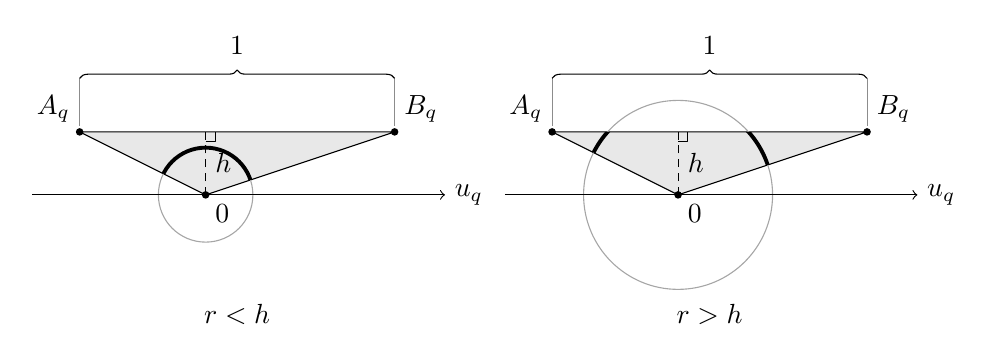
\begin{tikzpicture}[x=4cm,y=4cm,line join=round]
\foreach \rad/\shift/\tag in {0.15/0/{r<h},0.30/6/{r>h}} {
 \begin{scope}[xshift=\shift cm]
  \coordinate (O) at (0,0);
  \coordinate (Far) at (0.6,0.2);
  \coordinate (Near) at (-0.4,0.2);
  \fill[black!9] (O)--(Far)--(Near)--cycle;
  \draw[thin] (O)--(Far)--(Near)--cycle;
  \draw[black!35] (O) circle (\rad);
  \begin{scope}
   \clip (O)--(Far)--(Near)--cycle;
   \draw[line width=1.4pt] (O) circle (\rad);
  \end{scope}
  \draw[densely dashed] (O)--(0,0.2) node[midway,right] {$h$};
  \draw[thin] (0,0.17)--(0.03,0.17)--(0.03,0.2);
  \draw[->,thin] (-0.55,0)--(0.76,0) node[right] {$u_q$};
  \draw[black!45,thin] (-0.4,0.22)--(-0.4,0.37) (0.6,0.22)--(0.6,0.37);
  \draw[decorate,decoration={brace,amplitude=3pt}] (-0.4,0.37)--(0.6,0.37)
    node[midway,above=5pt] {$1$};
  \fill (O) circle (0.012) node[below right] {$0$};
  \fill (Far) circle (0.012) node[above right] {$B_q$};
  \fill (Near) circle (0.012) node[above left] {$A_q$};
  \node at (0.10,-0.38) {$\tag$};
 \end{scope}
}
\end{tikzpicture}
\caption{同一完整单位针在两个半径上的截面。浅色是原点三角形，粗圆弧是它的实际圆周截面。左图的圆周尚未达到底边，远端和近端使用同一完整角域；右图的圆周跨过底边后，截面分成两条端部弧。对两个端点计数，不意味着可以将左图的同一条粗弧计算两次。}
\label{fig:needle-sections}
\end{figure}


% [G04]
特别地，对每个 $0<r<M$，都有一个实际的远端基区间
\begin{equation}
 J_r(q)=
 \begin{cases}
 [b,d],&r\leq z,\\
 [b,\min\{d,a_r\}],&z<r<M.
 \end{cases}
\label{eq:core-far-base}
\end{equation}
第二种情形下，它的长度为 $\min\{\gamma,a_r-b\}$。这个最小值保证了垂足落在底边外时，区间仍处于实际角域之内。将此基区间向角度 $0$ 延伸，只需增加长度 $b$，便到达底边的理想远端方向。

% [G05]
若 $z=0$，三角形就是从 $0$ 到 $x$ 的径向区间；在 $x<1$ 时，还包含反方向长为 $1-x$ 的径向区间。对 $0<r<M=x$，取实际远端射线在圆周上的单点作为基区间。它已与理想远端锚点重合，无需延伸。上述径向区间均为闭区间，所以在 $r=M$ 时仍保留远端方向的单点；存在反向径向区间时，其正半径端点也被保留。这类方向可能构成方向测度为正的集合，因此下文每个并集估计都保留它们。

\begin{lemma}[远端截面下界]
\label{lem:core-far}
设一个 Borel 单位线段族满足 $M\geq m\geq1/2$。再设存在固定的有限常数 $B\geq0$，使其中所有 $z>0$ 的成员都满足 $b/\gamma\leq B$。那么，该族的每个 Borel 方向子集 $V$ 都满足
\begin{equation}
 |S_r(V)|\geq
 \min\left\{\frac1{1+2B},\frac{m-r}{m+r}\right\}|V|,
                   \qquad 0<r<m.
\label{eq:core-far-kernel}
\end{equation}
\end{lemma}

\begin{proof}
% [G06]
对 $0<t\leq1$，比值 $\arcsin(t)/t$ 单调递增，因为它是递增函数 $(1-v^2)^{-1/2}$ 在 $[0,t]$ 上的平均值。若 $z<r<M$，则 $b=\arcsin(z/M)$，因而
\[
 \frac{b}{a_r}\leq\frac rM,\qquad
 \frac{b}{a_r-b}\leq\frac r{M-r}\leq\frac r{m-r}.
\]
对实际基区间 \eqref{eq:core-far-base}，延伸长度与基区间长度之比因此不超过
\[
                   \rho=\max\{B,r/(m-r)\}.
\]
分母取两个候选长度的最小值，所得比值就是相应两个比值的最大值；完整角域情形下，比值不超过 $B$。零高度的单点区间也满足这一延伸条件。

% [G07]
对所有这些实际基区间一次性应用引理~\ref{lem:core-interval}。它们的并集包含于 $S_r(V)$，延伸后的并集则包含 $V$ 中每个方向的一个按 Borel 规则选出的理想远端提升。这个提升集的长度为 $|V|$，所以
\[
                  |V|\leq(1+2\rho)|S_r(V)|.
\]
取 $1+2\rho$ 的倒数，就得到 \eqref{eq:core-far-kernel}。这一次应用已经同时处理了正、负高度，完整角域、较短的端部弧，以及它们在平面中的所有重叠。
\end{proof}

\begin{lemma}[由端点半径上界控制角域]
\label{lem:core-bounded}
设
\[
 0<H\leq1/2,\qquad m\geq1/2,\qquad
 R\geq\max\{m,\sqrt{1/4+H^2}\},
\]
且一个 Borel 族满足 $m\leq M\leq R$ 和 $|h|\leq H$。那么，对每个 Borel 方向子集 $V$ 及 $0<r<m$，都有
\begin{equation}
 |S_r(V)|\geq
 \min\left\{K(R,H),\frac{m-r}{m+r}\right\}|V|,
 \qquad
 K(R,H)=\frac{\sqrt{R^2-H^2}}{\sqrt{R^2-H^2}+2R^2}.
\label{eq:core-bounded-kernel}
\end{equation}
\end{lemma}

\begin{proof}
% [G08]
对 $z>0$，角域张角为
\[
 \gamma=\int_{x-1}^{x}\frac{z}{t^2+z^2}\,dt.
\]
由于 $x\geq1/2$，每个 $t\in[x-1,x]$ 都满足 $|t|\leq x$。于是 $\gamma\geq z/M^2$；再由 $b\leq z/x$ 得
\[
                     \frac b\gamma\leq\frac{M^2}{x}
                                           =x+\frac{z^2}{x}.
\]
固定 $z\leq H\leq1/2$ 后，最后一个表达式在 $x\geq1/2$ 上递增，因为它的导数为 $1-z^2/x^2\geq0$。约束 $M\leq R$ 给出 $x\leq\sqrt{R^2-z^2}$，故
\[
 \frac b\gamma\leq\frac{R^2}{\sqrt{R^2-z^2}}
                  \leq\frac{R^2}{\sqrt{R^2-H^2}}.
\]
用这个 $B$ 值应用引理~\ref{lem:core-far} 即可。假设保证了各分母为正，也保证了放宽后的 $(x,z)$ 定义域中所用的上端点可行。这个积分论证同时包含垂足在底边内部和外部的情形。
\end{proof}

\subsection{在内圆盘中使用满足条件的近端点}
\label{subsec:core-low}

% [L01]
将满足 $M<99/100$ 的方向称为低半径方向，记它们组成的 Borel 集为 $L$。在 $L$ 上，式~\eqref{eq:core-endpoints} 给出 $1/2\leq x<1$，所以每条底边都跨过自己的垂足。固定任意 Borel 子集 $V\subseteq L$，将它分成
\begin{equation}
 B(V)=\{q\in V:N(q)\geq2/5\},\qquad U(V)=V\setminus B(V).
\label{eq:core-eligible-split}
\end{equation}
对 $V$ 的每个方向都选取远端点，并且仅在 $B(V)$ 上再选取近端点。每个被选端点的半径都至少为 $2/5$。虽然各端点半径随方向变化，这个共同阈值仍允许我们只作一次延伸估计。

\begin{lemma}[可选端点给出的下界]
\label{lem:core-eligible}
对每个 Borel 子集 $V\subseteq L$ 及 $0<r<2/5$，都有
\begin{equation}
 |S_r(V)|\geq k_4(r)\bigl(|V|+|B(V)|\bigr),\qquad
 k_4(r)=\min\left\{\frac23,\frac{2/5-r}{2/5+r}\right\}.
\label{eq:core-eligible}
\end{equation}
\end{lemma}

\begin{proof}
% [L02]
先控制将完整角域延伸到选定锚点所需的长度。对 $z>0$，记
\[
 b=\arctan(z/x),\quad c=\arctan\bigl(z/(1-x)\bigr),\quad
 \gamma=\pi-b-c.
\]
实际角域为 $[b,\pi-c]$。向远端和近端延伸，分别需要长度 $b$ 和 $c$。我们断言，整个低半径族都满足 $b/\gamma<1/4$，包括那些近端点未被选取的方向。

% [L03]
固定 $0<z\leq1/5$，只需证明 $5b+c<\pi$。若 $1/2\leq x\leq4/5$，则
\[
 b\leq z/x\leq2/5,\qquad
 c=\arctan\bigl(z/(1-x)\bigr)\leq\arctan1=\pi/4,
\]
故 $5b+c\leq2+\pi/4<\pi$。若 $4/5<x<1$，则
\[
 b\leq z/x\leq1/4,\qquad c<\pi/2,
\]
从而 $5b+c<5/4+\pi/2<\pi$。这两种情况都只用了非负参数上的 $\arctan t\leq t$、反正切的单调性和 $\pi>3$。于是 $4b<\pi-b-c=\gamma$，证明了远端的四分之一延伸界，不要求近端点可选。

若近端点被选取，则 $M\geq N\geq2/5$，因此
\[
 \sin b=z/M\leq1/2,\qquad \sin c=z/N\leq1/2.
\]
两个角都在 $(0,\pi/2)$ 内；由该区间上正弦的严格单调性和 $\sin(\pi/6)=1/2$，得 $b,c\leq\pi/6$。因而 $\gamma\geq2\pi/3$ 且 $c/\gamma\leq1/4$。这后一条界只用于近端点确实可选的方向。

% [L04]
现在固定 $r\in(0,2/5)$。对满足 $r\leq z$ 的成员，将整个角域作为每个选定端点的实际基区间。若两端点都被选取，就把同一个角域列出两次，分别向两侧延伸；每次都至多延伸基区间长度的四分之一。对满足 $0<z<r$ 的成员，令 $a=\arcsin(z/r)$。选定的实际端部弧在远端为 $[b,a]$，在符合条件的近端为 $[\pi-a,\pi-c]$。它们都是完整的端部弧，因为底边跨过垂足，且选定端点半径 $R_e$ 满足 $R_e\geq2/5>r$。记 $\beta=\arcsin(z/R_e)$，则延伸长度为 $\beta$，实际基区间长度为 $a-\beta$；与前面一样，
\[
 \frac{\beta}{a}\leq\frac r{R_e},\qquad
 \frac{\beta}{a-\beta}\leq\frac r{R_e-r}
                                  \leq\frac r{2/5-r}.
\]
对 $z=0$ 的成员，将每条选定的实际射线在圆周上的单点作为基区间。其半径至少达到 $2/5$，所以该点确实属于半径为 $r$ 的截面，且无需延伸。

% [L05]
所有这些基区间都在同一个实际截面 $S_r(V)$ 中。它们可以完全重合：对一条两个端点均可选的非零高度针，若 $0<r<z$，远端与近端所用的基区间都是同一完整角域 $[b,d]$。下面增加的是理想锚点的数目，不是另有一份不相交的实际角域。对整个族应用引理~\ref{lem:core-interval}，取
\[
                    \rho=\max\{1/4,r/(2/5-r)\}.
\]
延伸后的并集包含 $V$ 的理想远端提升，以及 $B(V)$ 的反向理想近端提升。这两个提升集互不相交：若两个实际角度锚点相等，它们的射影方向就必相等，但同一方向的两个锚点互为对径点。由第~\ref{subsec:core-intervals} 节的坐标区间论证，两者的长度分别为 $|V|$ 和 $|B(V)|$。所以
\[
           |V|+|B(V)|\leq(1+2\rho)|S_r(V)|,
\]
从而证明了 \eqref{eq:core-eligible}。新增项计数的是互异的理想锚点；测量长度之前，每个实际角域或端部弧都已与所有重叠基区间合并。
\end{proof}

% [L06]
对 $U(V)$ 中的方向，有 $N<2/5$，由 $M+N\geq1$ 得 $M>3/5$。这些方向少了第二个选定锚点，却有半径更大的远端点。对 $1/5<r<1/2$，每个非零高度都满足 $0<z<r$，且底边跨过垂足，因此远端弧完整，不受角域截断。沿用同一个延伸证明，每个方向只使用一个远端锚点，得到
\begin{align}
 |S_r(V)|&\geq k_5(r)|V|,
 &k_5(r)&=\frac{1/2-r}{1/2+r},\label{eq:core-k5}\\
 |S_r(U(V))|&\geq k_6(r)|U(V)|,
 &k_6(r)&=\frac{3/5-r}{3/5+r}.\label{eq:core-k6}
\end{align}
第一个不等式使用的端点半径下界是 $1/2$，第二个是 $3/5$。零高度方向仍贡献各自实际的单点锚点。在这些半径上无需完整角域估计。

% [L07]
现在将这三个截面下界积分，并让同一块面积只被使用一次。在 $(0,1/5)$ 上使用满足条件的双端点估计，在 $[1/5,7/20)$ 上使用全体远端点估计 \eqref{eq:core-k5}。在余下的区间 $[7/20,1/2)$ 上，\eqref{eq:core-k5} 和 \eqref{eq:core-k6} 都可用，但相应并集可能重叠。选择 $\lambda\in[0,1]$，赋予它们互补权重：
\begin{equation}
 \lambda\mathbf1_{W(U(V))}+(1-\lambda)\mathbf1_{W(V)}
                            \leq\mathbf1_{W(V)}.
\label{eq:core-complement}
\end{equation}
由于 $W(U(V))\subseteq W(V)$，这个不等式逐点成立。在较小的并集上，总权重恰为一；在 $W(V)$ 的其余部分，权重为 $1-\lambda$。

% [L08]
定义以下正的积分常数
\begin{align}
 C_4&=\int_0^{1/5}r k_4(r)\,dr,&
 C_5&=\int_{1/5}^{7/20}r k_5(r)\,dr,\nonumber\\
 C_6&=\int_{7/20}^{1/2}r k_6(r)\,dr,&
 D_5&=\int_{7/20}^{1/2}r k_5(r)\,dr.
\label{eq:core-four-integrals}
\end{align}
每个被积函数在相应区间内部都为正，故这些常数为正。在此圆盘内，$\nu$ 就是通常面积。将式~\eqref{eq:core-eligible}--\eqref{eq:core-complement} 分别在对应的半径区间上积分，记 $b_V=|B(V)|$ 和 $u_V=|U(V)|$，得到
\begin{align}
 |W(V)\cap D(0,1/2)|
 &\geq C_4(2b_V+u_V)+C_5(b_V+u_V)\nonumber\\
 &\hspace{9mm}+\lambda C_6u_V+(1-\lambda)D_5(b_V+u_V).
\label{eq:core-low-ledger}
\end{align}
这里及下文均以 $D(0,a)$ 表示开圆盘；改变所用区域的边界圆周归属，不影响面积。

% [L09]
在 \eqref{eq:core-low-ledger} 中，$b_V$ 与 $u_V$ 的系数之差为 $C_4-\lambda C_6$。因此，精确选择
\begin{equation}
 \lambda=\frac{C_4}{C_6},\qquad
 C_* =2C_4+C_5+\left(1-\frac{C_4}{C_6}\right)D_5
\label{eq:core-price}
\end{equation}
便能平衡两类方向，条件是 $C_4<C_6$。这个选择与 $V$ 无关，也不依赖于近端点可选的方向占比。下面全程使用有理数界，核验它的取值范围以及定理所需的数值阈值。

\begin{lemma}[内圆盘贡献的精确大小]
\label{lem:core-constants}
式 \eqref{eq:core-four-integrals} 中的常数满足
\[
 0<C_4<C_6,\qquad
 C_*>\frac{637}{20000}>\frac{71}{2230}>\frac1{10\pi}.
\]
因此，每个 Borel 子集 $V\subseteq L$ 都满足
\begin{equation}
                 |W(V)\cap D(0,1/2)|\geq C_*|V|.
\label{eq:core-low-result}
\end{equation}
\end{lemma}

\begin{proof}
% [A01]
多项式除法给出原函数
\[
 Q_m(r)=-\frac{r^2}{2}+2mr-2m^2\log(1+r/m),\qquad
 Q_m'(r)=\frac{r(m-r)}{m+r}.
\]
$k_4$ 的两个分支在 $r=2/25$ 处相等。先将常数分支积分至该点，再使用 $Q_{2/5}$，并在其余区间分别使用 $Q_{1/2},Q_{3/5}$，得到
\begin{align}
 C_4&=\frac{61}{750}-\frac8{25}\log\frac54,
 &C_5&=\frac{87}{800}-\frac12\log\frac{17}{14},\nonumber\\
 C_6&=\frac{93}{800}-\frac{18}{25}\log\frac{22}{19},
 &D_5&=\frac{69}{800}-\frac12\log\frac{20}{17}.
\label{eq:core-four-closed}
\end{align}
特别地，系数 $D_5$ 来自低半径圆盘同一外侧区域内余下的全体远端点贡献，而不是另一个圆环。

% [A02]
下面给出这些对数比较的有理数证书。对 $a>1$，令 $t=(a-1)/(a+1)$，并定义
\[
 L(t)=2\sum_{j=0}^{39}\frac{t^{2j+1}}{2j+1},\qquad
 T(t)=\frac{2t^{81}}{81(1-t^2)}.
\]
对 $2/(1-t^2)$ 的几何级数积分，得到
\begin{equation}
                    L(t)<\log a<L(t)+T(t).
\label{eq:core-log-certificate}
\end{equation}
事实上，被略去的级数每项都为正，其和至多为 $2\sum_{j\geq40}t^{2j+1}/81=T(t)$；在 $t>0$ 时严格小于这个上界。下表中四个 $t$ 都是 $(0,1)$ 内的有理数。若一行的形式为 $C=p-c\log a$，证书给出的下、上界依次为 $p-c(L(t)+T(t))$ 和 $p-cL(t)$，顺序来自 $c>0$。以下较粗的界已经足够：
\[
\begin{array}{c|c|c|c|c|c}
 C&p&c&t&10^6\,\underline C&10^6\,\overline C\\ \hline
 C_4&61/750&8/25&1/9&9927&9928\\
 C_5&87/800&1/2&3/31&11671&11672\\
 C_6&93/800&18/25&3/41&10695&10696\\
 D_5&69/800&1/2&3/37&4990&4991
\end{array}
\]
更明确地说，每一行断言以下有限的有理数不等式：
\begin{equation}
 \underline C<p-c(L(t)+T(t))<C<p-cL(t)<\overline C.
\label{eq:core-rational-rows}
\end{equation}
因此，证书由上述有限和及正的几何余项组成；核验时只需消去正整数分母，不必用小数近似对数。

% [A03]
由表中各行可得 $0<C_4<C_6$，故 $0<\lambda<1$。这些有理数界还给出
\[
 C_*>
 \frac{2\cdot9927+11671}{10^6}
 +\left(1-\frac{9928}{10695}\right)\frac{4990}{10^6}
 >\frac{637}{20000}.
\]
上式最后一个有理数比较乘以 $10^6\cdot10695$ 后，正差可写为
\[
 (2\cdot9927+11671-50\cdot637)10695
                         +(10695-9928)4990>0.
\]
例如，在前一个下界中将 $(10695-9928)/10695$ 换成更小的 $7/100$，也能看出这个差为正。互补权重和 $D_5$ 都为正，因此可以将它们的下界相乘。

% [A04]
为使计算完整，初等下界 $\pi>223/71$ 也可以不用 $\pi$ 的小数值来证明。正切加法公式给出
\[
 \frac\pi4=4\arctan\frac15-\arctan\frac1{239};
\]
右端的角位于 $(0,\pi/2)$，且正切为一。使用反正切的交错级数，第一个级数截到负的第四项，第二个以首项作上界，得到
\[
 \pi>
 16\left(\frac15-\frac1{3\cdot5^3}
                  +\frac1{5\cdot5^5}-\frac1{7\cdot5^7}\right)
          -\frac4{239}>\frac{223}{71}.
\]
这里最后一步是分母为正的有理数不等式。再比较目标阈值：
\[
 \frac{637}{20000}-\frac{71}{2230}=\frac{51}{4460000}>0,
 \qquad \frac{71}{2230}>\frac1{10\pi}.
\]
将 \eqref{eq:core-price} 代入 \eqref{eq:core-low-ledger} 后，两类方向的系数恰好都为 $C_*$，从而证明 \eqref{eq:core-low-result}。在 $|V|=0$ 时，面积比较仍是所需的非严格不等式。这不意味着实际并集的面积为零：若 $V=\{q\}$ 且该三角形非退化，则 $|V|=0$ 而 $|W(V)|=|h|/2>0$；对 $0<r<|h|$，其完整角域的长度也为正。此时变成零的只是下界中的方向因子。
\end{proof}

\subsection{将其余方向分配到尚未使用的圆环}
\label{subsec:core-high}

% [H01]
内圆盘现在已贡献至少 $|L|/(10\pi)$。对其余方向，定义
\begin{equation}
 F=\{99/100\leq M<8/5\},\qquad
 D_n=\{m_n\leq M<2m_n\},\quad
 m_n=\frac85\,2^n,\quad n\geq0.
\label{eq:core-partition}
\end{equation}
这些集合与 $L$ 一起构成覆盖整个方向圆周的 Borel 划分。对 $F$，只在 $[1/2,4/5)$ 上积分；对 $D_0$，只在 $[4/5,6/5)$ 上积分；对每个 $n\geq1$，只在 $[m_n/2,m_n)$ 上积分。这些半径区间与低半径圆盘互不相交，彼此也互不相交。区间 $[6/5,8/5)$ 留空不用。

\paragraph{端点半径在 $99/100$ 与 $8/5$ 之间。}
% [H02]
对 $F$ 应用引理~\ref{lem:core-bounded}，取 $m=99/100$、$R=8/5$ 和 $H=1/5$。各参数满足引理的条件，且 $[1/2,4/5)$ 内的所有半径都小于 $m$。常数分支为
\[
 K_F=\frac{5\sqrt{63}}{5\sqrt{63}+128}>\frac7{30}.
\]
为核验这个严格不等式，交叉相乘后只需证明 $115\sqrt{63}>896$。两边都为正，平方后所得差为
\[
                         115^2\cdot63-896^2=30359.
\]
有理函数分支 $(99/100-r)/(99/100+r)$ 随 $r$ 递减。在下表三个区间的右端点，其值与所列系数之差依次为 $19/1590$、$0$ 和 $0$：
\[
\begin{array}{c|c}
 \hbox{半径区间}&k\ \hbox{用于 }|S_r(F)|\geq k|F|\\ \hline
 {[1/2,3/5)}&7/30\\
 {[3/5,7/10)}&29/169\\
 {[7/10,4/5)}&19/179
\end{array}
\]
三个系数都不超过 $7/30$，因此角域分支也高于它们。

% [H03]
半径小于一时，极坐标权重为 $r$。对表中三行积分，得到
\begin{align}
 \nu\bigl(W(F)\cap\{1/2\leq|x|<4/5\}\bigr)
 &\geq I_F|F|,\nonumber\\
 I_F&=\frac7{30}\frac{(3/5)^2-(1/2)^2}{2}
      +\frac{29}{169}\frac{(7/10)^2-(3/5)^2}{2}\nonumber\\
 &\hspace{9mm}+\frac{19}{179}\frac{(4/5)^2-(7/10)^2}{2}
       =\frac{446059}{13962000}.
\label{eq:core-finite-payment}
\end{align}
由精确比较
\[
 \frac{223}{71}I_F-\frac1{10}
                    =\frac{340957}{991302000}>0
\]
以及 $\pi>223/71$，可得 $I_F>1/(10\pi)$。每行使用同一个并集 $W(F)$ 的不同圆环；在这些半径上，不再重复使用该并集的面积。

\paragraph{第一个更大端点半径类。}
% [H04]
对 $D_0$，在同一引理中取 $m=8/5$、$R=16/5$ 和 $H=1/5$。引理的条件同样满足，垂足位于底边外的线段也在适用范围内。其常数分支满足
\[
 K_0=\frac{5\sqrt{255}}{5\sqrt{255}+512}>\frac18,
 \qquad 35^2\cdot255-512^2=50231>0.
\]
这里交叉相乘得到 $35\sqrt{255}>512$，因此平方差为正就证明了所需比较。在整个 $[4/5,6/5)$ 上，有理函数分支不小于右端点处的值
\[
                     \frac{8/5-6/5}{8/5+6/5}=\frac17>\frac18.
\]
所以该区间上有 $|S_r(D_0)|\geq|D_0|/8$。这个区间跨过半径一，而 \eqref{eq:core-nu} 中的密度在此改变，因此其贡献为
\begin{equation}
 \nu\bigl(W(D_0)\cap\{4/5\leq|x|<6/5\}\bigr)
 \geq I_0|D_0|,\qquad
 I_0=\frac18\left(\int_{4/5}^{1}r\,dr+
                          \int_1^{6/5}1\,dr\right)=\frac{19}{400}.
\label{eq:core-first-tail}
\end{equation}
仅用 $3I_0-1/10=17/400>0$ 就已足够，故 $I_0>1/(10\pi)$。

\subsection{覆盖所有后续尺度的端部短段估计}
\label{subsec:core-tail}

% [T01]
对于任意大的端点半径，不必再使用固定的角域估计。在底边上靠近远端点取一小段，它会留在指定的较小圆周外。沿径向填充后，这一小段的整个角度像都进入三角形的截面。下一个引理估计这些像的并集，不假设不同短段的像互不相交。

\begin{lemma}[远端短段]
\label{lem:core-collar}
设一个 Borel 单位线段族满足 $m\leq M\leq R$，其中 $m>1/2$。那么，每个 Borel 方向子集 $V$ 都满足
\begin{equation}
 |S_r(V)|\geq
 \frac{\min\{1/2,m-r\}}{\pi R}|V|,
                                      \qquad 0<r<m.
\label{eq:core-collar}
\end{equation}
\end{lemma}

\begin{proof}
% [T02]
固定 $0<t\leq1/2$。从每个远端点沿底边朝另一端点取长为 $t$ 的一段，称为端部短段。由反三角不等式，短段上每一点的半径都至少为 $m-t>0$；又由半径为 $R$ 的圆盘的凸性，其半径至多为 $R$。记这些短段的角度像之并为 $P_t(V)$。短段及其角度像均有 Borel 参数化，因此 $P_t(V)$ 是解析集，从而可测。我们先证明
\begin{equation}
                        |P_t(V)|\geq\frac{t}{\pi R}|V|.
\label{eq:core-collar-image}
\end{equation}

% [T03]
取包含 $P_t(V)$ 的开角度集 $O$。若 $O$ 是整个圆周，由 $|V|\leq\pi$ 和 $R>t$ 就有 $|V|\leq\pi R|O|/t$。否则，将 $O$ 分成可数个开弧连通分支。每个端部短段的角度像都连通，故包含于某个分支 $C$，记其长度为 $\ell$。若 $\ell\geq t/R$，全体射影方向的长度也只有 $\pi\leq\pi R\ell/t$，足以估计这个分支对应的方向集。

% [T04]
若 $\ell<t/R<1$，记 $C$ 的中点角度为 $c$。端部短段的两端点半径都至多为 $R$，角度与 $c$ 的距离都不超过 $\ell/2$。将短段端点写成 $X_i=r_i(\cos\theta_i,\sin\theta_i)$，在开弧 $C$ 的一次展开中有 $|\theta_i-c|\leq\ell/2$。垂直于角度 $c$ 的单位向量为 $n_c=(-\sin c,\cos c)$，所以 $X_i\cdot n_c=r_i\sin(\theta_i-c)$，绝对值至多为 $R\sin(\ell/2)$。又因 $X_1-X_0$ 是沿方向 $q$ 的长为 $t$ 的向量，其投影长度恰为 $t|\sin(q-c)|$。两端点投影之差不超过各自绝对值之和。因此，与这个分支对应的每个方向都满足
\[
                  t|\sin(q-c)|\leq2R\sin(\ell/2).
\]
令 $\eta=2R\sin(\ell/2)/t$。由 $\sin(\ell/2)\leq\ell/2$，得 $0\leq\eta\leq R\ell/t<1$。把 $q-c$ 的模 $\pi$ 代表取在 $[-\pi/2,\pi/2)$ 内，$|\sin(q-c)|\leq\eta$ 就等价于 $|q-c|\leq\arcsin\eta$。因此这个射影方向集的长度为 $2\arcsin\eta$。引理~\ref{lem:core-far} 的证明已经说明 $t\mapsto\arcsin(t)/t$ 递增。与 $t=1$ 的取值 $\pi/2$ 比较，就有 $\arcsin\eta\leq\pi\eta/2$；$\eta=0$ 时等号成立。因此，这个方向集的长度至多为 $\pi R\ell/t$。

% [T05]
因此，每个分支都对应一个长度至多为 $\pi R\ell/t$ 的可测方向集，包含所有分配到该分支的端部短段方向。这里取测度的是上述显式正弦带（较长分支则使用整个方向圆周），而不是另行选择的源子集；只须这些可测集合的可数并覆盖 $V$。将长度相加，得 $|V|\leq\pi R|O|/t$，再对 $O$ 取下确界，就证明了 \eqref{eq:core-collar-image}。这个论证也包含角度像为单点的径向短段。

% [T06]
最后固定 $r\in(0,m)$，取 $t=\min\{1/2,m-r\}$。此时每个端部短段上的点半径都至少为 $r$。原点与该点之间的线段属于相应的三角形，因此该点的角度属于 $S_r(V)$。于是 $P_t(V)\subseteq S_r(V)$，由 \eqref{eq:core-collar-image} 即得引理。三角形包含边界线段，因此径向下界取等号时，结论仍成立。
\end{proof}

% [T07]
对 $n\geq1$ 的 $D_n$，应用端部短段引理，取 $m=m_n$ 和 $R=2m_n$，并且只使用半径区间 $[m_n/2,m_n)$。得到
\[
 |S_r(D_n)|\geq\frac{\min\{1/2,m_n-r\}}{2\pi m_n}|D_n|.
\]
这里 $m_n\geq16/5$，所以整个区间的半径都大于一，$\nu$ 的极坐标权重为 $1$。被积函数在 $r=m_n-1/2$ 之前恒为 $1/2$，随后线性降至零。它的积分等于整个区间上的矩形面积，减去末端缺少的三角形面积：
\[
 \int_{m_n/2}^{m_n}\min\{1/2,m_n-r\}\,dr
                                   =\frac{m_n}{4}-\frac18.
\]
因此
\begin{equation}
 \nu\bigl(W(D_n)\cap\{m_n/2\leq|x|<m_n\}\bigr)
 \geq C_n|D_n|,\qquad
 C_n=\frac1\pi\left(\frac18-\frac1{16m_n}\right).
\label{eq:core-later-tails}
\end{equation}
括号内的表达式随 $m_n$ 递增。在最小允许值 $m_n=16/5$ 处，它等于 $27/256$，且
\[
                      \frac{27}{256}-\frac1{10}=\frac7{1280}>0.
\]
所以，对每个 $n\geq1$ 都有 $C_n>1/(10\pi)$。同一公式覆盖所有后续尺度，半径可以任意大。

\subsection{相加实际贡献，再取外测度}
\label{subsec:core-closure}

\begin{proof}[定理~\ref{thm:core-tenth} 的证明]
% [Z01]
固定第~\ref{subsec:core-recovery} 节中的开超集 $G$ 及重新选出的族。存在高度足够大的三角形时，已经得到 $|G|\geq1/10$。否则，所有高度均满足 \eqref{eq:core-height}，前面的引理适用于划分 $L,F,D_0,D_1,\ldots$。定义以下实际可测子集
\begin{align*}
 A_L&=W(L)\cap\{|x|<1/2\},\\
 A_F&=W(F)\cap\{1/2\leq|x|<4/5\},\\
 A_0&=W(D_0)\cap\{4/5\leq|x|<6/5\},\\
 A_n&=W(D_n)\cap\{m_n/2\leq|x|<m_n\},\qquad n\geq1.
\end{align*}
这些集合的半径范围两两不交，因为后续区间的第一个是 $[8/5,16/5)$，以后每个区间都从前一个的右端点开始。因此，逐点有
\begin{equation}
       \mathbf1_{A_L}+\mathbf1_{A_F}+\sum_{n\geq0}\mathbf1_{A_n}
                                                   \leq\mathbf1_W
\label{eq:core-final-capacity}
\end{equation}
低半径圆盘的估计已经遵守了内部互补权重条件 \eqref{eq:core-complement}；这里仅对 $V=L$ 使用一次它的结论。

% [Z02]
对 \eqref{eq:core-final-capacity} 关于 $\nu$ 积分。无论是否有无穷多个非空方向类，非负函数的单调收敛定理都允许取这个可数和。所用的是方向类互不相交且总长度为 $\pi$；不要求 $|D_n|$ 几何递减。几何增长的是半径阈值 $m_n$。由于 $W\subseteq G$ 且 $\nu$ 的密度不超过一，
\begin{align*}
 |G|\ &\geq\nu(W)\\
 &\geq\nu(A_L)+\nu(A_F)+\sum_{n\geq0}\nu(A_n)\\
 &\geq C_*|L|+I_F|F|+I_0|D_0|+\sum_{n\geq1}C_n|D_n|\\
 &\geq\frac{|L|+|F|+\sum_{n\geq0}|D_n|}{10\pi}
       =\frac1{10}.
\end{align*}
最后一个等号用到方向划分覆盖整个圆周，以及 $|\mathbb {RP}^1|=\pi$；所有截面长度则始终在长度为 $2\pi$ 的实际角度圆周上测量。对某个具体的只取有限个中点值的重选族，端点半径事实上有界，但这个可数求和论证不需要这样的界。

% [Z03]
我们已对每个开集 $G\supseteq E$ 证明 $|G|\geq1/10$。对这些开集的测度取下确界，便得 $|E|^*\geq1/10$。所有三角形和辅助可测并集都构造在 $G$ 内，因此这最后一步直接适用于原来的任意集合 $E$。
\end{proof}

\section{下界留下的极值问题}\label{sec:extremal}
第~\ref{sec:core-tenth} 节给出了适用于所有容许集合的下界。要确定锐值，还需要一列合法集合的面积趋近同一个值。我们先把这些构造所用的有限语言写清。

% [U002]
记 $u_q=(\cos q,\sin q)$、$n_q=(-\sin q,\cos q)$，并以 $B_R$ 表示以原点为中心、半径为 $R$ 的闭圆盘。
一个\emph{原始有限体}是形如下式的集合：
\begin{equation}\label{eq:upper-original}
 K=\bigcup_{i=1}^{M}\ \bigcup_{q\in I_i}
 \operatorname{conv}\left(0,
 (b_i+[-1/2,1/2])u_q+h_i n_q\right),
 \qquad \bigcup_{i=1}^{M}I_i=\mathbb {RP}^1,
\end{equation}
其中 $I_i$ 是闭方向区间，$b_i,h_i$ 在每条记录上均为常数。
更换射影方向的提升时，把 $(q,b_i,h_i)$ 换成 $(q+\pi,-b_i,-h_i)$，实际线段保持不变。
在共用端点处保留两侧的记录。
以 $A_*$ 表示这些有限体的面积 $|K|$ 的下确界；$M$ 和外包半径都不设上界。


经典 Cunningham--Schoenberg 构造给出星形问题的族上界
\[
 A_*\le \frac{5-2\sqrt2}{24}\,\pi
\]
\cite{CunninghamSchoenberg1965}。原文通过充分大的奇数指标和任意小的正误差实现这一估计，并没有断言极小值达到；下文将从完整针的源轮廓出发研究更细的面积比较。

\begin{lemma}[开包络中的有限恢复]\label{lem:finite-open-recovery}
设 $S$ 是有限外面积的原点星形集，在每个射影方向上都含有一条完整闭单位线段。对任意开集 $O\supset S$，存在原始有限体 $F\subset O$。特别地，对任意 $\varepsilon>0$，可使 $|F|<|S|^*+\varepsilon$。
\end{lemma}
\begin{proof}
对每个方向 $q$，选出一条完整单位线段 $N_q\subset S$。三角形 $T_q=\operatorname{conv}(0,N_q)$ 是 $O$ 内的紧集，退化时也一样。由旋转在这个紧集上的一致连续性，存在 $0<\delta_q<\pi/4$，使 $|\alpha|\le\delta_q$ 时旋转后的整个三角形仍在 $O$ 内。这里不要求对所有 $q$ 有统一的角宽或半径界。

取 $q$ 的一个实数提升 $t_q$。由 $|\alpha|<\delta_q/2$ 定义的开射影弧覆盖方向圆周，因而有有限子覆盖。用相应的、已经验证安全的较宽闭弧 $|\alpha|\le\delta_q$ 定义 $F$，即取这些旋转三角形的并。每一片都是紧参数积的连续像，相对于旋转坐标系的 $b,h$ 保持常数。因此 $F$ 是紧的原始有限体，接缝记录保留，且每个方向都有一条完整的旋转单位线段留在 $F$ 内。又因 $F\subset O$，有 $|F|\le|O|$。最后由外正则性取 $|O|<|S|^*+\varepsilon$，即得面积结论。
\end{proof}
所需紧性属于每个三角形和方向圆周，而不属于整个 $S$；所以引理也适用于无界的 Borel 代表元及不可测输入。它保证单位覆盖和向上的面积逼近；保留一条指定运动所需的包含恢复将在后文另行证明。

若比较涉及某个固定操作，恢复输入还不够：对恢复后输入施加同一操作所得的输出，也必须满足所需面积比较。第~\ref{sec:shear} 节会同时控制这两端。严格改进一个给定构造，或证明候选族的每个成员都能改进，回答的仍是较小的问题：可得的节省可能随复杂度增加而消失。锐值比较需要对其所作用的近极小序列保留足够的统一控制。

原有限类还可以附加一项要求：在体内选出随方向连续、首尾闭合的完整单位针。第~\ref{subsec:upper-coherent} 节将其面积下确界记为 $A_{\mathrm{coh}}$；这个符号始终指原有限相干子类。紧星体作为更广的测试对象会出现在连续化障碍定理中，但不会改变这一下确界的定义。


连续的方向选择也须与一般的时间参数运动区分。去掉共同星形中心后，即使要求方向参数化连续，单位段的并仍可包含在任意小测度的紧集中~\cite[定理~3.3]{JarvenpaaEtAl2011}。因此，本问题的正面积约束不能仅由选择函数的连续性解释。


\section{几何替换必须支付什么}\label{sec:replacement-bank}
以下比较的实际并集均可测且面积有限。
设一个构造保留背景 $B$，撤去一批并集为 $P$ 的三角形，再插入新的完整单位针，其三角形的并集为 $Q$。面积变化恰好是
\begin{equation}\label{eq:physical-change}
 |B\cup Q|-|B\cup P|=|Q\setminus B|-|P\setminus B|.
\end{equation}
把每个并集分成保留的背景及其外部部分，就得到这个恒等式。这个恒等式也能用来诊断替换。一个三角形可能缩小，但它原来占用的材料被许多其他三角形重复覆盖，而替换物落到了所有其他三角形外。此时把各来源的节省相加，算出的既不是式~\eqref{eq:physical-change} 的左边，也不是右边。

对紧致原点星形体，同一套面积核算可以写成极坐标形式。若 $\rho_K(\phi)$ 是它在实际射线 $\phi$ 上的径向延伸长度，则
\[
 |K|=\frac12\int_0^{2\pi}\rho_K(\phi)^2\,d\phi.
\]
所有记录都在定义 $\rho_K$ 的同一个径向上确界中竞争。来源方向 $q$ 与实际射线 $\phi$ 的作用不同：一个测度为零的方向标签仍可能贡献一个非退化三角形，而一条记录可以占据一整个实际射线区间。下面的例子会保留这些三角形，而不随标签一起将它们丢掉。

成功的上界构造恰好利用了这种竞争。它们的纵向分拆同时移动两个端点的相位，而有符号高度把完整底边的部分放到已经存在的三角形后面。随后的高度和纵向变分移去暴露的条带，同时把补偿材料留在已有的径向延伸范围内。最后的弦长延长步骤使用体内实际包含的整个区间，而不只是两个可见端点。一致的删去量在有限恢复之前就已得到保证。显式构造及其严格比较需要各自的几何假设；替换恒等式解释了这些比较为什么有意义，却不提供那些假设。


% 完整中文精修稿；由冻结的 upper_zh_initial.tex 逐句修改而来。
% 需要支持中文的主文档，以及 amsmath、amssymb、amsthm 和 theorem、lemma、proposition 环境。
% 段落编号用于 upper_zh_sentence_audit.md，不排入正文。

\section{完整源线段与严格上界改进}
\label{sec:upper-constructions}

% [U001]
缩短长臂未必节省面积：其他针可能已经覆盖它失去的全部部分。
反过来，延长互补臂也未必增加面积，只要新增的整个三角形都在已有径向上边界之下。
两种效应都可利用，节省多少却必须由所得并集的面积判断。
对不受限问题最强的比较来自一个整弦操作：先延长集合内的整条弦，再以星心为中心缩回单位长度。

\begin{theorem}[严格上界构造]\label{thm:upper-chain}
存在下文定义的固定源轮廓及其实际面积代价，使得
\begin{equation}\label{eq:upper-chain}
 A_*\le c_{\mathrm{hl}}-\Gamma_{\mathrm{ms}}
 <c_{\mathrm{hl}}<c_{\mathrm{height}}<c_r<c_{\mathrm{fr}}<U,
 \qquad U=0.284167531115949,
\end{equation}
其中 $\Gamma_{\mathrm{ms}}>0$ 是固定常数。
另有一个独立构造的代价 $c_{\mathrm{new}}<c_{\mathrm{fr}}$，满足 $A_*\le c_{\mathrm{new}}$。

$c_{\mathrm{fr}},c_r,c_{\mathrm{height}},c_{\mathrm{hl}},c_{\mathrm{new}}$ 各自都是一个指定全源族的面积极限，也都能由原始有限体逼近。
对于弦归一化后的输出，只断言嵌套的上极限估计。
常数 $U$ 是已有证书确认的历史基准；本定理中后续各个差值均不在这里作数值求值。
\end{theorem}

% [U003]
式~\eqref{eq:upper-chain} 中的符号表示不同的集合或不同的极限，并非同一个数的逐次小数近似。
特别地，论证不使用 $c_{\mathrm{new}}$ 与 $c_r$ 或后续代价之间的比较。
我们先构造实际面积极限，再比较互补臂的代价，最后使正面积节省在两次离散化后仍然保留。

\subsection{周期记录包含整条线段}
\label{subsec:upper-periodic}

% [U004]
设 $p:[0,1]\to(0,1)$ 连续且满足 $p(1-t)=1-p(t)$；设 $h:[0,1]\to[0,\infty)$ 连续，满足 $h(1-t)=h(t)$ 及 $h(0)=h(1)=0$。
对 $y=j+t$、$j\in\mathbb Z$、$0\le t\le1$，令
\begin{equation}\label{eq:upper-periodic-data}
 P(y)=\frac12+(-1)^j\left(p(t)-\frac12\right),
 \quad M(y)=1-P(y),\quad A(y)=(-1)^{j+1}h(t).
\end{equation}
端点恒等式保证这些定义在整数接缝处一致。
这些函数以二为周期，并满足 $P(y+1)=M(y)$、$A(y+1)=-A(y)$。
对奇数 $n$，令 $\delta_n=\pi/n$，并定义
\begin{equation}\label{eq:upper-actual-source}
 N_{n,y}=\{xu_{\delta_n y}+\delta_n A(y)n_{\delta_n y}:
                 -M(y)\le x\le P(y)\},\qquad
 E_n[p,h]=\bigcup_{0\le y\le n}\operatorname{conv}(0,N_{n,y}).
\end{equation}
由 $P+M=1$，每条底边的长度都是一，而其方向覆盖 $[0,\pi]$。
交替放置并不要求加入对径集合 $-E_n$。

% [U005]
沿底边点向原点填充，就在同一角度上得到所有更小的半径。
这里的相位是将实际角度按尺度 $\delta_n$ 展开后取模二的坐标；有限角度的精确公式见下面的证明。
固定极限半径 $\rho>0$ 后，要得到完整截面，就须让纵向坐标从 $\rho$ 遍历到臂端点，而非只取端点值。
在带有总质量为二的长度测度的 $\mathbb T_2=\mathbb R/2\mathbb Z$ 上，定义
\begin{align}
 S_+^{p,h}(\rho)&=\bigcup_{\substack{0\le y\le2\\P(y)\ge\rho}}
 \{y+A(y)/x\pmod2:\rho\le x\le P(y)\},\\
 S_-^{p,h}(\rho)&=\bigcup_{\substack{0\le y\le2\\M(y)\ge\rho}}
 \{y-A(y)/x\pmod2:\rho\le x\le M(y)\}.
\end{align}
这个完整源族的\emph{实际极限代价}为
\begin{equation}\label{eq:upper-physical-cost}
 C_{\mathrm{phys}}(p,h)=\frac\pi2\int_0^\infty
 \rho\bigl(|S_+^{p,h}(\rho)|+|S_-^{p,h}(\rho)|\bigr)\,d\rho.
\end{equation}
这是并集的积分，不是源三角形面积之和，也不是端点包络的替代量。
关系 $S_-+1=S_+$ 说明二者的相位长度相同，并不把实际平面中的两个半平面等同起来。

\begin{proposition}[两阶段实际面积恢复]\label{prop:upper-recovery}
对本节使用的每一对固定轮廓，即冻结的多项式对及下文构造的有限分片代数或多项式修改，均有
\[
 \lim_{\substack{n\to\infty\\n\ \mathrm{odd}}}|E_n[p,h]|
       =C_{\mathrm{phys}}(p,h).
\]
对每个固定奇数 $n$，存在原始有限体 $K_{n,k}[p,h]$，满足
\[
 \lim_{k\to\infty}|K_{n,k}[p,h]|=|E_n[p,h]|.
\]
网格尺度趋于零，并细分所有源分片边界；每个闭小源区间上，都在同一个代表参数处取 $b=(-1)^j(p-1/2)$ 和带符号高度 $\delta_n(-1)^{j+1}h$ 的值，再同时冻结。
并集中保留接缝两侧的所有闭记录。
\end{proposition}

\begin{proof}
% [U006]
令 $H=\max_{[0,2]}|A|$，并固定满足 $\delta_nH<\rho$ 的 $\rho>0$。
正臂的精确定义域与相位为
\[
 \sqrt{\rho^2-\delta_n^2A(y)^2}\le x\le P(y),\qquad
 y+\delta_n^{-1}\arctan\bigl(\delta_n A(y)/x\bigr).
\]
负臂使用 $M$，并将反正切前的符号反转。
因此，在取极限之前，真实半径和底边的完整内部都已保留。
避开 $P$ 和 $M$ 的有限多个临界值、常值分片值及接缝值后，所有激活端点都是横截的。
这些连通定义域在上述扰动下持续存在，且对充分大的 $n$，其上有 $x\ge\rho/2$。
相位一致收敛到 $y\pm A(y)/x$。
连通定义域的实相位像是完整区间；极值收敛先给出各区间长度收敛，再给出它们模二后的有限并集长度收敛。

% [U007]
在这个固定正半径上，相位位移有界，所以把无限周期源截为 $[0,n]$ 只会改变有界个数的首尾单元。
这些首尾单元的实际角宽趋于零。
分别计入正负两侧的实际区域，得到极限角长度 $\frac\pi2(|S_+|+|S_-|)$。
所有集合都在同一个圆盘中，每个圆周截面的角长度至多为 $2\pi$。
半径为 $\rho_0$ 的圆盘把整个小半径部分的贡献控制在 $\pi\rho_0^2$ 以内，再由控制收敛定理得到式~\eqref{eq:upper-physical-cost}。

% [U008]
固定 $n$ 后，端点的一致逼近使 $K_{n,k}$ 落在紧集 $E_n$ 逐渐缩小的外邻域内，从而得到面积的上极限估计。
对于下极限，每个非退化源三角形的内点都在其冻结近似中持续存在。
逐个考察闭解析源坐标片，也包括代数端点处的收敛 Puiseux 坐标片：端点曲线 $e$ 要么只有有限多个 $\det(e,e')$ 的零点，要么位于一条固定射线上。
在非临界的侧边点处，略微改变源参数，就能把该点的严格径向缩点移入相邻三角形的内部。
例外的侧边射线只有有限条；在其余每条射线上，只有最外端点可能不属于三角形内部的并集。
有限条例外射线的面积为零；在其余每条射线上，遗漏的至多一个最外端点也有一维径向测度零。极坐标 Fubini 定理因而说明整个遗漏集的面积为零。
记非退化源三角形内部的并为 $\mathcal I_n$，则 $|\mathcal I_n|=|E_n|$，且 $\mathbf1_{\mathcal I_n}\le\liminf_k\mathbf1_{K_{n,k}}$ 逐点成立；Fatou 引理给出面积的下极限估计。
正高度源端点始终保留其完整三角形；测度论证中略去的只有上述边界射线。
由此得到的是实际面积收敛；论证没有借 Hausdorff 收敛代替面积收敛。
\end{proof}

% [U009]
冻结的轮廓对为 $p_0=1/2+\alpha_{\mathrm{fr}}$ 与 $s$；本节末尾列出 $\alpha_{\mathrm{fr}}$ 和 $s$ 按幂次递增排列的精确系数。
定义 $c_{\mathrm{fr}}=C_{\mathrm{phys}}(p_0,s)$。
电子符号证书与包络证书给出了下文使用的严格凹性、反射关系、开盒约束、两个严格起始不等式及递增端点映射，也给出了历史比较 $c_{\mathrm{fr}}<U$。
附录~\ref{sec:formal-evidence} 按数学输入列出这些证据的对应关系；它们只支持上述固定输入，不能推广为所有同次数多项式都满足这些不等式。

\subsection{互补臂产生凸铰链函数}
\label{subsec:upper-hinge}

% [U010]
固定 $s\in C^2([0,1])$，满足 $s(1-t)=s(t)$、$s(0)=s(1)=0$，且在 $[0,1]$ 上有 $s''<0$。
满足反射关系的放置函数 $p\in C^1([0,1])$ 称为\emph{起始可容许}，若它在整个闭区间上满足 $0<p<1$，并且满足
\begin{equation}\label{eq:upper-birth}
 p(t)>\frac{s(t)}t,\qquad
 1-p(t)>\frac{s(t)}{1-t}\qquad(0<t<1).
\end{equation}
令 $d=s'(0)$、$g(t)=t-s(t)/p(t)$。第一个起始不等式给出 $g(t)>0$，第二个对反射臂给出同样的结论：两条臂的端点相位都已经越过各自的零相位。再令
\begin{equation}\label{eq:upper-tail-threshold}
 T_s(z)=\max_{0\le u\le1}\frac{s(u)}{u+z}\quad(z>0),
 \qquad B_s(t)=\max_{0\le u\le1}\frac{s(t)+s(u)}{t+u}\quad(t>0),
\end{equation}
其中在零点以连续延拓定义 $T_s(0)=B_s(0)=d$。
$T_s(z)$ 描述相位 $-z$ 上的径向上边界：在内部源 $0<u<1$ 处解 $u-s(u)/x=-z$，得到 $x=s(u)/(u+z)$。起始条件保证这个底边坐标合法。
因此，只要高度轮廓相同，每个起始可容许放置都包含同一个负相位尾部；反射后，它也参与正相位上的比较。

\begin{lemma}[阈值与完整径向上边界]\label{lem:upper-roof}
对 $0<t\le1$，定义 $B_s(t)$ 的最大值由唯一的源参数 $u_t\in(0,\min(t,1/2))$ 取得，且
\[
 B_s(t)=s'(u_t),\qquad
 B_s'(t)=\frac{s'(t)-B_s(t)}{t+u_t},\qquad
 d>B_s(t)>\frac{s(t)}t>s'(t).
\]
对任意起始可容许的 $p$，定义
\[
 \tau(z)=\min\{t\in[0,1]:g(t)\ge z\},\qquad 0<z<1.
\]
完整正向径向上边界为 $R(z)=p(\tau(z))$，实际代价为
\begin{equation}\label{eq:upper-roof-cost}
 C_{\mathrm{phys}}(p,s)=\pi\int_0^1\max\{R(z),T_s(z)\}^2\,dz.
\end{equation}
若臂长 $x>s(t)/t$，则它与互补尾部的比较满足
\[
 x>T_s(t-s(t)/x)\quad\Longleftrightarrow\quad x>B_s(t).
\]
将两边都改成等号或都反转不等号，同样等价。
\end{lemma}

\begin{proof}
% [U011]
阈值商对源参数求导后的分子为 $(t+u)s'(u)-s(t)-s(u)$。
这个分子对 $u$ 的导数为 $(t+u)s''(u)<0$，在 $u=0$ 和 $u=t$ 处符号相反。
它在 $1/2$ 处为负，因而极大源具有所述位置且唯一；随后隐式求导给出各恒等式。
与 $T_s$ 的比较来自恒等式
\[
 x(u+t-s(t)/x)-s(u)=x(t+u)-s(t)-s(u),
\]
这里使用了分母为正以及最大值能够取到。

% [U012]
起始条件给出 $g(0)=0$、$g(1)=1$，并在内部给出 $0<g(t)<t$，所以 $\tau(z)$ 存在且 $g(\tau(z))=z$。
一条完整正底边只有在满足 $g(u)\ge z$ 的源参数 $u$ 处才能到达相位 $z$，对应半径为 $s(u)/(u-z)$。
在第一个这样的源参数处，导数分子 $(u-z)s'(u)-s(u)$ 为负，此后还会严格递减。
所以，即使合法源集合不连通，每个更晚的合法源给出的半径也都更小。
这就在不丢弃底边内点的前提下证明了首次到达的径向上边界公式。
负相位给出 $T_s$，反射给出另一侧的提升；由于 $T_s$ 递减，第一个单元中每个更远的等价相位表示也都受 $T_s(z)$ 控制。
第二个单元由相应反射得到，再计入实际平面的两侧，就得到式~\eqref{eq:upper-roof-cost}。
\end{proof}

% [U013]
定义铰链函数及其反射配对形式为
\begin{align}
 \Phi_s(t,x)&=(x-B_s(t))_+^2
             +2(B_s(t)-s'(t))(x-B_s(t))_+,\\
 \Psi_t(x)&=\Phi_s(t,x)+\Phi_s(1-t,1-x),
 \qquad m_s(t)=\min_{0\le x\le1}\Psi_t(x),\\
 L(s)&=\pi\left(\int_0^1T_s(z)^2\,dz+
                         \int_0^{1/2}m_s(t)\,dt\right).
\end{align}
这里 $v_+=\max(v,0)$。
铰链函数是凸的，但一般在 $x=B_s(t)$ 处不可微。
线性项不可省略：零代价臂一旦延伸越过阈值，就立即增加暴露面积。

\begin{theorem}[铰链比较及几何等号条件]\label{thm:upper-hinge}
设 $p$ 起始可容许，且 $\min_{[0,1]}g'>0$。
则
\begin{equation}\label{eq:upper-hinge-identity}
 C_{\mathrm{phys}}(p,s)=\pi\left(\int_0^1T_s^2+
                                      \int_0^1\Phi_s(t,p(t))\,dt\right)
 \ge L(s).
\end{equation}
对 $0\le t\le1/2$，令 $b=B_s(t)$、$\bar b=B_s(1-t)$、$\sigma=s'(t)$。
若 $b+\bar b\ge1$，则 $\Psi_t$ 的极小点集为 $[1-\bar b,b]$，最小值为零。
若 $b+\bar b<1$，则其唯一极小点为
\[
 x_t=\operatorname{clamp}\left(\frac12+\sigma,[b,1-\bar b]\right),
\]
其中对 $v\le w$，定义 $\operatorname{clamp}(x,[v,w])=\min(w,\max(v,x))$。
对于已经满足本定理几何假设的放置，等号成立当且仅当每个 $t\in[0,1/2]$ 处的 $p(t)$ 都属于相应极小点集。
\end{theorem}

\begin{proof}
% [U014]
令 $H(z)=\int_0^zT_s(w)^2\,dw$，并在 $x>B_s(t)$ 时定义
\[
 F(t,x)=s(t)(x-B_s(t))-H(t-s(t)/x)
                         +H(t-s(t)/B_s(t));
\]
在 $x\le B_s(t)$ 时把 $F$ 延拓为零。
由阈值恒等式，拼接曲线上 $F$ 及其两个一阶偏导数都为零。
因此，链式法则穿过任意接触集仍然成立，并给出
\begin{equation}\label{eq:upper-primitive}
 (p^2-T_s(g)^2)_+g'
       =\frac{d}{dt}F(t,p(t))+\Phi_s(t,p(t)).
\end{equation}
沿曲线的导数有界，且 $F$ 在两端都趋于零，故其导数积分不产生边界项或奇异项。
在式~\eqref{eq:upper-roof-cost} 中通过递增映射 $g$ 换元，即得恒等式。

% [U015]
第一个激活铰链的导数是 $2(x-\sigma)$，第二个的导数是 $-2(1-x+\sigma)$。
如果阈值区间重叠，两个铰链都在共同区间上为零。
两阈值之间若留有间隙，配对导数在间隙内为 $4x-2-4\sigma$；在间隙外向间隙移动，函数值总会下降。
由此得到上述截断极小点，也包括边界情形。
最后，反射关系将完整铰链积分写成 $\int_0^{1/2}\Psi_t(p(t))\,dt$，逐点比较便证明了下界。
这里没有把几何可行函数上的下确界移入积分。
\end{proof}

% [U016]
$L(s)$ 给出这个源类的松弛下界，是否能作为最小值取到还要检验几何条件。
拟议的极小放置仍须按要求的正则性拼接，满足起始条件，并满足
\[
 J_p(t):=p(t)^2-p(t)s'(t)+s(t)p'(t)>0,
 \qquad g'=J_p/p^2.
\]
逐点凸极小化不会自动保证这个微分条件。

\begin{proposition}[松弛最小值不可达的非空类]
\label{prop:upper-unattainable}
对每个 $\kappa\in(0,1/4)$，选择 $\varepsilon>0$ 使得
\[
 \kappa^2\frac{\sqrt{\varepsilon^2+1/4}-\varepsilon}{\varepsilon}>\frac14,
\]
并令
\[
 s(t)=\kappa\left(\sqrt{\varepsilon^2+1/4}
                -\sqrt{\varepsilon^2+(t-1/2)^2}\right).
\]
定理~\ref{thm:upper-hinge} 中的类非空，但其中 $C_{\mathrm{phys}}(p,s)$ 的下确界严格大于 $L(s)$。
\end{proposition}

\begin{proof}
% [U017]
这里 $|s'|<\kappa$ 且 $B_s\le d<\kappa$，所以 $p=1/2$ 满足起始条件以及 $g'>1-2\kappa>0$。
在整个区间上，唯一的逐点极小放置为 $p_*=1/2+s'$。
它满足起始条件和反射关系，但
\[
 J_{p_*}(1/2)=\frac14-
 \kappa^2\frac{\sqrt{\varepsilon^2+1/4}-\varepsilon}{\varepsilon}<0.
\]
此外，每个配对铰链在盒区间上的分布二阶导数至少为二，故代价趋近 $L(s)$ 会迫使 $p_j\to p_*$ 于 $L^2$。
取一个几乎处处收敛的子列后，非递减函数 $g_j=t-s/p_j$ 也会几乎处处收敛到 $g_*=t-s/p_*$。
这种极限有一个非递减代表元，而连续函数 $g_*$ 在 $1/2$ 附近严格递减。
这一矛盾排除了固定高度、端点映射递增的类中的任何恢复序列。
\end{proof}

\subsection{折叠对应精确的实际面积余项}
\label{subsec:upper-fold}

\begin{theorem}[有序交叉余项]\label{thm:upper-fold}
沿用第~\ref{subsec:upper-hinge} 节中 $s\in C^2([0,1])$ 的严格凹性、反射关系及零端点条件，并设 $p\in C^1([0,1])$ 起始可容许。这里仅撤去 $\min_{[0,1]}g'>0$ 的要求，允许 $g'$ 改变符号。
对几乎每个 $z\in(0,1)$，它的根依次为
\[
 t_1<\cdots<t_{2k+1},\qquad g(t_i)=z,
\]
导数符号按 $+,-,+,\ldots,+$ 交替。
定义 $w_i(z)=\max\{p(t_i)^2,T_s(z)^2\}$，并定义
\begin{equation}\label{eq:upper-fold-def}
 D_{\mathrm{fold}}(p,s)=\pi\int_0^1
               \sum_{j=1}^{k}\bigl(w_{2j}(z)-w_{2j+1}(z)\bigr)\,dz.
\end{equation}
则
\begin{equation}\label{eq:upper-fold-identity}
 C_{\mathrm{phys}}(p,s)-L(s)=
 \pi\int_0^{1/2}\bigl(\Psi_t(p(t))-m_s(t)\bigr)\,dt
                 +D_{\mathrm{fold}}(p,s),\qquad D_{\mathrm{fold}}\ge0.
\end{equation}
此外，$D_{\mathrm{fold}}=0$ 当且仅当在开激活集 $\{t\in(0,1):p(t)>B_s(t)\}$ 上有 $g'\ge0$。
这一公式也适用于连续 Lipschitz 放置，只要它由有限个闭 $C^1$ 分片组成，并在各分片的激活内部使用同一导数条件。
\end{theorem}

\begin{proof}
% [U018]
临界集 $\{g'=0\}$ 的像的长度为零：用 $\{|g'|<\eta\}$ 覆盖它，在这个开集的区间分支上估计像的长度，再令 $\eta$ 递减到零。
非临界值处的根孤立，由紧性知根只有有限个；又由 $g(0)<z<g(1)$，其导数符号交替。
引理~\ref{lem:upper-roof} 还给出更强的几何次序
\[
 p(t_1)>p(t_2)>\cdots>p(t_{2k+1}).
\]
将首次到达半径与尾部半径取大后平方，再减去带符号交叉和，恰为
\[
 w_1-\sum_{i=1}^{2k+1}(-1)^{i+1}w_i
              =\sum_{j=1}^k(w_{2j}-w_{2j+1})\ge0.
\]
保证余项非负的是这个半径次序，无须给重叠重数设上界。

% [U019]
令 $M_s=\max(\|p\|_\infty,d)$；逐分支换元将带绝对值的加权交叉积分控制在 $M_s^2\int_0^1|g'|$ 以内。
因此，即使折叠次数没有统一上界，带符号计算仍然可积。
恒等式~\eqref{eq:upper-primitive} 是逐点链式法则，不要求 $g'>0$。
此时尾部项通过 $H(g(1))-H(g(0))$ 积分，而不是通过保向换元积分。
这些恒等式证明了式~\eqref{eq:upper-fold-identity}。
各光滑分片的原函数在接缝处取值相同，内部边界项因而逐一抵消；平坦分片和接缝处都不产生原子项。

% [U020]
如果每个向下交叉都未激活，它的半径及其后向上交叉处更小的半径都不超过 $T_s$，这一对的贡献便为零。
反之，若某个激活点处有 $g'<0$，连续性就给出一个激活的递减区间，其像具有正长度。
该像中几乎每个相位都有一个严格高于尾部的向下交叉，其后跟着半径更小的向上交叉，因此对应差值为正。
这就证明了零余项判据的两个方向。
命题~\ref{prop:upper-unattainable} 中的针族在这个扩大类中是合法的，但中央的激活折叠使 $D_{\mathrm{fold}}(p_*,s)>0$。
单个放置的余项为正，并不能推出 $L(s)$ 与扩大类的下确界之间存在正间隙。
\end{proof}

% [U021]
从同一个参考放置 $p_0$ 出发，可以作两种朝向铰链极小点的投影；它们给出的放置不同。
记 $B=B_s$，定义
\begin{align}
 r(t)&=\operatorname{median}\bigl(B(t),p_0(t),1-B(1-t)\bigr),\label{eq:upper-band}\\
 q(t)&=\begin{cases}
 \operatorname{clamp}(1/2+s'(t),[B(t),1-B(1-t)]),&B(t)+B(1-t)<1,\\
 r(t),&B(t)+B(1-t)\ge1.
 \end{cases}\label{eq:upper-completed}
\end{align}
这里的中位数是三个实数参数中居中的一个，不预设两个阈值的大小次序。
$q$ 和 $r$ 都满足反射关系及开盒约束，都是 Lipschitz 有限分片放置，并满足严格内部起始条件。
事实上，若 $\ell=s(t)/t$、$V=1-s(t)/(1-t)$，则 $\ell<p_0<V$、$B>\ell$、$1-B(1-t)<V$；无论两个阈值怎样排序，投影到它们之间都保留这两个严格不等式。
两阈值相遇时，投影区间收缩为单点，这也保证了交界处的连续性。

% [U022]
补全后的选择函数满足
\[
 C_{\mathrm{phys}}(q,s)=L(s)+D_{\mathrm{fold}}(q,s),
\]
命题~\ref{prop:upper-recovery} 又将这个实际代价恢复为有限体的面积极限。
它的激活折叠余项是否为零，仍是开放问题。
未补全选择函数 $\operatorname{median}(B,1/2+s',1-B(1-t))$ 的内部起始条件仍未解决；已经证明的 $q$ 的起始性质不能移用到它身上。
这两个未决问题都不妨碍对另一个放置 $r$ 作严格的实际面积比较。

\subsection{冻结的高次放置为何不是驻点}
\label{subsec:upper-polynomial}

\begin{theorem}[多项式接触刚性与下降]\label{thm:upper-polynomial}
设多项式 $s$ 和 $p$ 满足定理~\ref{thm:upper-hinge} 的全部假设，并设 $\deg p>\deg s'\ge1$。
则在满足反射关系、起始可容许且 $g$ 的导数有正下界的 $C^1$ 类中，$p$ 不是 $C_{\mathrm{phys}}(\cdot,s)$ 的局部极小点。
存在任意小的 $C^1$ 扰动，具有紧内部支集和有限个多项式分片，并严格降低实际代价。
对于冻结轮廓对，$\deg p_0=19$、$\deg s'=15$，所以固定其中一个扰动即可定义
\[
 c_{\mathrm{new}}:=C_{\mathrm{phys}}(p_0+\epsilon v,s)<c_{\mathrm{fr}}.
\]
\end{theorem}

\begin{proof}
% [U023]
假设次数大于 $\deg s'$ 的多项式 $Q$ 在某个开区间上与 $B_s$ 一致。
阈值恒等式在该区间给出
\[
 \mathcal R(t)=\frac{s'(t)-Q(t)}{Q'(t)}-t=u_t,
 \qquad s'(\mathcal R(t))=Q(t).
\]
清除分母后，这成为复数域上的有理恒等式。
若约分后的 $\mathcal R$ 有有限极点，将它代入非常数多项式 $s'$，就会产生一个无法抵消的最高阶极点。
所以 $\mathcal R$ 是多项式。
若 $m=\deg Q$，它在无穷远处的首项行为为 $-(1+1/m)t$，因此次数为一。
它与 $s'$ 的复合于是具有次数 $\deg s'$，与 $\deg Q>\deg s'$ 矛盾。
反射同样排除了它与 $1-B_s(1-t)$ 在开区间上接触的可能。

% [U024]
由 $g'(0)>0$ 得 $p(0)>d=B_s(0)$，故零点附近有一个第一个铰链激活的区间。
去掉第二个铰链的闭接触集以及 $p-1/2-s'$ 的有限多个零点，选取紧区间 $I=[a_0,b_0]\subset(0,1/2)$，使铰链激活状态固定，且
\[
 D(t):=\partial_x\Psi_t(p(t))
 =\begin{cases}2(p-s'),&\text{仅第一个铰链激活},\\
                 4p-2-4s',&\text{两个铰链都激活}
   \end{cases}
\]
与零保持正距离。
在 $I$ 上令 $w(t)=(t-a_0)^2(b_0-t)^2$，在 $I$ 外令其为零。
在 $I$ 上取 $v=-\operatorname{sign}(D)w$，按 $v(1-t)=-v(t)$ 反射延拓，其余处置零。
端点的二重零点使 $v$ 在全局为 $C^1$。
扰动方向必须按实际配对导数选取，不能一律按 $p-1/2-s'$ 选取。

% [U025]
对所有充分小的正 $\epsilon$，起始条件、开盒约束、激活状态和导数条件的严格裕量同时保留。
在这个未改变的激活区域内，精确的有限差分为
\[
 C_{\mathrm{phys}}(p+\epsilon v,s)-C_{\mathrm{phys}}(p,s)
     =\pi(\epsilon L_0+\epsilon^2Q_0),
\quad L_0=-\int_I|D|w<0,\quad Q_0=\int_I\nu w^2>0,
\]
其中单激活时 $\nu=1$，双激活时 $\nu=2$。
固定任意满足 $0<\epsilon<-L_0/Q_0$ 的可容许 $\epsilon$。
这样在 $n$ 和记录网格变化之前就固定了一个正的面积节省，即旧成本减去新成本，命题~\ref{prop:upper-recovery} 再把它传递到原始有限体。
\end{proof}

\subsection{带投影、被遮住的高度增量与第二次纵向下降}
\label{subsec:upper-profile-chain}

\begin{proposition}[固定带投影严格节省面积]
\label{prop:upper-band}
对于精确冻结的 $p_0,s$，式~\eqref{eq:upper-band} 中的放置 $r$ 满足
\[
 c_r:=C_{\mathrm{phys}}(r,s)<c_{\mathrm{fr}}.
\]
\end{proposition}

\begin{proof}
% [U026]
在源参数 $t$ 处，简记 $b=B_s(t)$、$v=1-B_s(1-t)$。
若 $b<v$，从下方投影只把正臂延长到 $b$，从上方投影只把负臂延长到 $1-v=B_s(1-t)$。
若 $v\le b$，从下方投影只把正臂延长到 $v\le b$，从上方投影只把负臂延长到 $1-b\le B_s(1-t)$。
四种情形都使每条被延长的臂止于自身阈值或其下方。
考察被延长的正臂中 $0<X\le B_s(t)$ 的坐标，令 $z=t-s(t)/X$。若 $t>0$ 且 $z\le0$，则 $X\le s(t)/t<p_0(t)$，这个底边点本来就在旧线段内；$t=0$ 时，$X\le B_s(0)=d\le p_0(0)$ 也给出同一包含。若 $z>0$，阈值等价关系给出 $X\le T_s(z)$。这些点均已属于旧的实际并集。
特别地，$0<t<1$ 时的相位 $z=0$ 给出 $X=s(t)/t>0$，并不表示纵向坐标 $X=0$；这样的底边点已在旧线段内，径向填充也仍在旧三角形内。
尾部已经作径向填充，因此新增的整个三角形都被遮住，而不仅是端点。
合并实际的反射提升及等价相位表示后，就得到全局实际面积不增。

% [U027]
附录~\ref{sec:formal-evidence} 所列的固定带区间支配输入，在整个源区间上给出
\[
 I_0=(2^{-20},2^{-19}),\qquad
 p_0(t)\ge B_s(t),\quad p_0(t)\ge1-B_s(1-t).
\]
证书在这里提供的是整个区间上的断言：端点映射将 $I_0$ 及其反射送入已认证的首段、末段支配范围，那里的驻定尾部候选又恰好等于 $T_s$。
多项式接触刚性使这两个不等式在某个非空开子区间 $J_0\subset I_0$ 上同时严格成立。
在那里 $r(t)<p_0(t)$，且原来的首次到达端点严格高于尾部。
由引理~\ref{lem:upper-roof}，每个更晚的合法底边坐标都严格更低；每条新增臂又都在共同尾部内。
因此，新集合失去了这个暴露端点。

% [U028]
一个端点缺失还不等于面积下降。先在低于该端点的某个正半径处截断相位--半径模型。
包括径向参数和有限多个相关等价相位表示在内，完整源定义域都是紧的，所以新并集在此处是闭的。
这个缺失点的某个邻域与新集合不交，旧的连续径向上边界却从下方填满其中一个非空开集。
其面积密度为 $\rho\,d\rho\,dz$ 的正倍数，因而失去的面积为正。
结合全局不增，就证明了严格比较。
\end{proof}

% [U029]
对于这个实际的 $r$，引理~\ref{lem:upper-roof} 的导数公式说明 $B_s(t)$ 与 $1-B_s(1-t)$ 都严格递减。冻结多项式 $p_0$ 的非递增性来自附录~\ref{sec:formal-evidence} 所列的单调性输入；它又是非常数多项式，若在两个不同参数处取值相同，非递增性就迫使它在两者之间恒定，进而成为常数多项式，矛盾。因此 $p_0$ 也严格递减。
对任意两个递增排列的参数，三个函数各自的下降量都有一个共同的正下界。中位数对每个坐标单调，且三坐标同时减去同一个数时中位数也减去该数，所以 $r$ 严格递减。
令 $P=r(0)$，仍记 $d=s'(0)$。
同一附录所列的端点与尾部界给出
\[
 d=\frac{107161751}{128520000}<\frac{21}{25},
 \qquad T_s(1)<\frac4{25},\qquad P>d.
\]
最后一个不等式来自 $B_s(0)=d$、$B_s(1)=T_s(1)$ 及 $p_0(0)>d$。
该尾部包围估计用的是输出相位 $1/2$ 对应的实际驻定源区间，以及冻结高度 $s(1/2)$；源参数中点不能直接当作这个输出相位。

\begin{proposition}[被端点上边界遮住的高度增量]
\label{prop:upper-height}
存在 $0<\alpha<\beta<1/2$ 及固定的 $\epsilon_h>0$，使得令
\[
 \psi(t)=\begin{cases}(t-\alpha)^3(\beta-t)^3,&\alpha\le t\le\beta,\\0,&\text{其余情形},\end{cases}
 \quad h_1(t)=\psi(t)+\psi(1-t),\quad a=s+\epsilon_h h_1,
\]
后，轮廓对 $(r,a)$ 保持反射关系、严格凹性和起始条件，且
\[
 c_{\mathrm{height}}:=C_{\mathrm{phys}}(r,a)<c_r.
\]
区间与振幅都预先固定，不依赖之后的奇数 $n$ 和有限网格。
\end{proposition}

\begin{proof}
% [U030]
对 $0<\rho<P$，$r$ 的严格递减性使激活源集成为一个前缀 $[0,\tau_\rho]$。
若 $\rho\le r(1)$，则 $\tau_\rho=1$；否则 $r(\tau_\rho)=\rho$。
以下 $b$ 取 $s$ 或 $a$；两者均对称、严格凹，端点为零，并满足起始条件。定义
\[
 L_b(\rho)=\max_{0\le t\le\tau_\rho}\bigl(b(t)/\rho-t\bigr),
 \qquad G_b(\rho)=\max_{0\le t\le\tau_\rho}\bigl(t-b(t)/r(t)\bigr).
\]
完整相位定义域的底部是连通前缀，每条竖直纤维也连通，因而相位像是整个区间 $[-L_b,G_b]$。
令 $M_b(\rho)=\max(L_b(\rho),G_b(\rho))$。
反射并集模二后的长度为 $2\min(1,M_b(\rho))$，因此
\begin{equation}\label{eq:upper-height-cost}
 C_{\mathrm{phys}}(r,b)=2\pi\int_0^P
      \rho\min(1,\max(L_b(\rho),G_b(\rho)))\,d\rho.
\end{equation}
定义 $L_b$ 的最大值也可在整个 $[0,1]$ 上取。内部极大源满足 $b'(t)=\rho$；严格凹性与 $b(0)=0$ 给出 $b(t)/t>b'(t)$，起始条件再给出 $r(t)>b(t)/t$，所以它已被激活。边界极大值只能在 $t=0$ 取得，而 $\rho<P=r(0)$ 保证它也被激活。

% [U031]
由 $P>d$，端点映射 $g_{r,s}=t-s/r$ 在足够短的起始邻域上，其几乎处处导数有一个正下界。
在 $\rho=d$ 处尾部最大值为零，而该邻域内一个足够小的正源参数给出 $G_s(d)>0$。
选闭窗口 $\mathcal N=[d-\eta,d+\eta]\subset(0,P)$，使其上有 $G_s-L_s>0$，并定义
\[
 \kappa_h=\frac14\min_{\rho\in\mathcal N}(G_s(\rho)-L_s(\rho))>0.
\]
在更小的起始邻域内选 $[\alpha,\beta]$，使 $r>d+\eta$、$s'$ 严格落在 $\mathcal N$ 内，且端点映射递增。
把 $\epsilon_h$ 选得足够小，使凹性、起始条件及该邻域上的递增性保留，使支集上的 $a'$ 留在 $\mathcal N$ 内，并满足
\[
 \epsilon_h\|h_1\|_\infty
       \left(\frac1{\min r}+\frac1{d-\eta}\right)<2\kappa_h.
\]
有限个紧集上的正裕量条件可同时满足，允许振幅因此包含一个非空区间。

% [U032]
对每个半径，由 $a\ge s$ 得 $G_a\le G_s$。
若 $L_a(\rho)>L_s(\rho)$，新的极大源只能落在正凸起内部；它满足 $a'(t)=\rho$，所以 $\rho$ 必在 $\mathcal N$ 内。
反射支集位于 $t>1/2$。总高度 $a$ 对称且严格凹，故其在这里的导数 $a'(t)<0$，不能满足正半径所需的极大值方程 $a'(t)=\rho>0$。这里不要求附加凸起自身的导数处处为负。
在 $\mathcal N$ 上，上述振幅约束保持 $G_a>L_a$，所以变化尾部的一切增量都被遮住。
在 $\mathcal N$ 外，尾部不变，端点占据也不增加。
这样，完整实际截面在所有半径上都不增加，极大源改变也不例外。

% [U033]
选一个非退化闭区间 $J\subset(\alpha,\beta)$。
在具有正宽度的半径区间 $r(J)$ 上，激活端点属于 $J$，两个端点映射都在整个激活前缀上递增，两个尾部都为零，且截面尚未饱和。
其损失恰为 $\epsilon_h\psi(\tau_\rho)/\rho$，故
\[
 c_r-c_{\mathrm{height}}
 \ge2\pi\epsilon_h\int_{r(J)}\psi(\tau_\rho)\,d\rho>0.
\]
区间的正宽度只需 $r$ 严格递减，不需要另给 $-r'$ 一个正下界。
\end{proof}

\begin{proposition}[固定新高度后的纵向下降]
\label{prop:upper-longitudinal}
对于刚构造并固定的 $a$，存在反射反对称的 $C^1$ 有限分片函数 $v_h$，其支集严格位于已有高度支集区间内部，并存在固定 $\eta_h>0$，使得
\[
 p_*=r+\eta_hv_h,\qquad
 c_{\mathrm{hl}}:=C_{\mathrm{phys}}(p_*,a)<c_{\mathrm{height}}.
\]
放置 $p_*$ 仍然严格递减、满足开盒约束和起始条件，并保留原端点值。
\end{proposition}

\begin{proof}
% [U034]
在已有高度支集的左边界 $\alpha$ 附近，有 $r>d>B_a$。
因此，有限分片中位数在 $\alpha$ 的某个右邻域上选取 $1-B_s(1-t)$ 或 $p_0$。
这就分成以下两种情形；纵向支集都在已经固定的高度凸起内部选取。
正的高度增量在其整个内部给出 $1-B_a(1-t)<1-B_s(1-t)$。

% [U035]
若 $r=1-B_s(1-t)$，在这个分支内选紧区间 $I=[a_h,b_h]$，并在 $I$ 上令 $w(t)=(t-a_h)^2(b_h-t)^2$，其余处置零。
在 $I$ 上取 $v_h=-w$，按 $v_h(1-t)=-v_h(t)$ 延拓，在两个支集之外置零。
这把暴露的正臂缩短，同时把互补臂延长相同的长度。
新互补臂仍在 $B_a(1-t)$ 以下，新增的整个三角形都被共同尾部遮住。
原递增邻域中的一个紧高半径带严格损失端点相位，正如式~\eqref{eq:upper-height-cost} 中的论证。
选中分支的导数在紧内部区间上严格为负，所以充分小的 $C^1$ 改动保留递减性和起始条件。
第一种情形由此完成，全局端点映射递增并非所需假设。

% [U036]
若 $r=p_0$，则 $a-s$ 及其一阶导数都在 $\alpha$ 和 $1-\alpha$ 处为零。
旧递增映射 $g_{p_0,s}$ 因而为 $g_{p_0,a}$ 提供两个局部递增邻域。
在每个邻域内选一个更早的截断点 $b$；对于所有更早的源，左侧有
\[
 g_{p_0,a}(u)\le g_{p_0,s}(u)\le g_{p_0,s}(b)
                          <g_{p_0,s}(\alpha)
\]
右侧在 $1-\alpha$ 处有相应的不等式。
将两个源支集选得足够靠近各自边界，使输出窗口既避开所有这些早期源的相位界，又彼此分离。

% [U037]
对支撑在这两个区间内的任意紧支集反射 $C^1$ 凸起 $v_h$，辅助放置 $q_\eta=p_0+\eta v_h$ 在小 $\eta$ 下仍保持这些严格相位间隙；检查后一个窗口时，较早的已修改窗口也受同一控制。
对未改变的源，若 $r\le p_0$，可与这个辅助映射比较；若 $r>p_0$，中位数给出 $r\le B_s\le B_a$，所以整条臂都被遮住。
更晚的合法源严格低于首次到达半径，因为 $a(u)/(u-z)$ 在首次到达后递减。
这些情形穷尽了更早、更晚及被遮住的源，证明新旧集合在两个窗口上的实际径向上边界均为 $\max(R,T_a)$。
这个辅助放置只承担相位比较，不要求 $(p_0,a)$ 在全局满足起始条件。

% [U038]
接触刚性仍在局部适用：每个高度分片的导数次数是十五，而 $p_0$ 的次数是十九。
实现阈值最大值的源参数随 $t$ 严格递增，因此可先避开其有限多个分片接缝，再使用定理~\ref{thm:upper-polynomial} 的有理复合证明。
令 $D_h=\partial_x\Psi^{a}_t(p_0(t))$，其中 $\Psi^{a}$ 是以高度 $a$ 构成的配对铰链。
选取避开接触点和 $D_h$ 零点的紧激活区域 $I=[a_h,b_h]$。
在 $I$ 上令 $w(t)=(t-a_h)^2(b_h-t)^2$，区间外置零；在该区间取 $v_h=-\operatorname{sign}(D_h)w$，再像第一种情形那样反射并补零。
每条被改变的完整底边条带，其相位介于新旧端点相位之间；随后径向填充不改变相位。
因此，局限在两个已验证窗口内的是全部实际几何变化，而不仅是端点变化。

% [U039]
在激活窗口上有 $p^2g'=p^2-pa'+ap'$，分部积分消去了凸起的导数。
把两个窗口配对，得到精确有限差分
\[
 C_{\mathrm{phys}}(r+\eta v_h,a)-C_{\mathrm{phys}}(r,a)
  =\pi(\eta L_h+\eta^2Q_h),\quad
 L_h=-\int_I|D_h|w<0,\quad Q_h=\int_I\nu w^2>0,
\]
其中按激活情形，$D_h=2(p_0-a')$ 或 $4p_0-2-4a'$，相应地 $\nu=1$ 或 $2$。
选一个正的 $\eta_h<-L_h/Q_h$，同时满足此前固定的起始、导数、相位间隙与激活区域裕量。
第一种情形改用紧尾部与起始邻域的裕量选 $\eta_h$，其正节省已由严格半径带论证保证。
两种情形都先固定 $p_*$ 和 $c_{\mathrm{hl}}$，然后再应用命题~\ref{prop:upper-recovery}。
\end{proof}

\subsection{在原始微观尺度上归一化整条弦}
\label{subsec:upper-chords}

% [U040]
一次性固定命题~\ref{prop:upper-longitudinal} 中的轮廓对 $(p_*,a)$，令 $g(t)=t-a(t)/p_*(t)$，并将其原始有限恢复简记为 $K_{n,k}$。
接下来的操作同时使用这个集合、它的原始记录以及 $\delta_n=\pi/n$。
这个操作依赖原始记录，仅凭未标记的集合不能确定。

% [U041]
对每条原始闭记录 $e=(i,q)$，记
\[
 N_e=[l_e,r_e]u_q+h_e n_q,\qquad r_e-l_e=1.
\]
在所有长度 $\ell=U-L\ge1$、整段包含于集合内的区间 $C=[L,U]u_q+Hn_q\subset K_{n,k}$ 中，施加约束
\begin{equation}\label{eq:upper-Q}
 (L-l_e)^2\le\ell-1,\qquad (U-r_e)^2\le\ell-1,
 \qquad \left(\frac{H-h_e}{\delta_n}\right)^2\le\ell-1.
\end{equation}
将 $\ell$ 最大化，对每条记录保留\emph{所有}极大解，并令
\begin{equation}\label{eq:upper-Q-output}
 S^Q_{n,k}=\overline{\bigcup_e\ \bigcup_{C\ \text{为记录 }e\text{ 的极大解}}
                              \operatorname{conv}(0,C/\ell)}.
\end{equation}
包含约束逐点检查整条区间；不连通直线截面中的两段，不能跨过孔洞合成一条弦。
规则只对旧集合执行一次，不按有利源筛选，也不迭代。

\begin{theorem}[归一化约束延长给出的固定实际面积删除]
\label{thm:upper-Q}
存在固定 $\Gamma_{\mathrm{ms}}>0$ 及整数 $N$，使每个奇数 $n\ge N$ 都有自己的 $k_0(n)$，并且所有原始细分 $k\ge k_0(n)$ 均满足
\[
 S^Q_{n,k}\subset K_{n,k},\qquad
 |K_{n,k}\setminus S^Q_{n,k}|\ge\Gamma_{\mathrm{ms}}.
\]
特别地，
\begin{equation}\label{eq:upper-Q-limit}
 \limsup_{\substack{n\to\infty\\n\ \mathrm{odd}}}
 \limsup_{k\to\infty}|S^Q_{n,k}|
                  \le c_{\mathrm{hl}}-\Gamma_{\mathrm{ms}},
 \qquad A_*\le c_{\mathrm{hl}}-\Gamma_{\mathrm{ms}}.
\end{equation}
$\Gamma_{\mathrm{ms}}$ 的一个精确定义是证明中所给正带积分的一半。
\end{theorem}

\begin{proof}
% [U042]
旧线段本身可行，紧性又使所含区间的坐标和长度全部有界。
整段包含关系在端点收敛下是闭的，式~\eqref{eq:upper-Q} 的三个约束也都是闭的，因此最大值存在。
每个 $C/\ell$ 的长度恰为一，并由星形性知它包含于 $K_{n,k}$；它的整个三角形以及这些三角形并集的闭包也都包含于其中。
方向、零高度记录、射影重提升以及并列极大解，一个也没有删去。
若 $\ell=1$，约束就迫使 $C=N_e$ 精确成立。

\paragraph{在每个实现上边界的源附近延长整条弦。}
% [U043]
在已选纵向激活区域内取嵌套紧区间，使较小区间包含某个紧的正则暴露相位区间 $Z\subset(0,1)$ 上的全部首次到达源参数。
旧支集端点满足 $r>d$，$p_*$ 在那里未变且严格递减，所以整个支集上都有 $p_*>d$。
其局部径向上边界 $R(z)=p_*(g^{-1}(z))$ 因而高于 $d$，并与共同尾部及非等价的相位表示分离。
此处只对已证明的局部首次到达映射取逆，并未假设全局可逆。
我们将在该上边界的\emph{每个}等价源表示的邻域上得到固定的长度下界。

% [U044]
互补臂被遮住时，它的端点严格位于实际尾部上边界之下。
单激活的多项式情形也包括在内。
尾部的极大源起始可容许，严格的尾部支配同时给出底边内部裕量和径向收缩裕量。
这给出一段真正连通的向外延续；它及其与旧线段的连接处，每一点都严格位于某个源三角形内部。
保留原来的整条线段，在同一支撑直线上接上一段足够短的这种延续段。
长度增益随延长量线性变化，约束中的纵向误差平方随延长量二次变化，法向误差为零，所以式~\eqref{eq:upper-Q} 带有严格裕量地成立。

% [U045]
双激活时，旧的两个端点都暴露在外，所需的较长区间必须移到邻近的支撑直线上。
在偶数单元内，源映射为
\[
 F_n(t,x)=\operatorname{Rot}_{\delta_n t}(x,-\delta_n a(t)),
                         \qquad p_*(t)-1\le x\le p_*(t).
\]
在 $t$ 处的坐标系中，相邻源 $u$ 的正端点坐标为
\begin{align}
 X_+(u;t)&=p_*(u)\cos(\delta_n(u-t))
                    +\delta_n a(u)\sin(\delta_n(u-t)),\\
 A_+(u;t)&=a(u)\cos(\delta_n(u-t))
                    -p_*(u)\frac{\sin(\delta_n(u-t))}{\delta_n},
\end{align}
其法向坐标为 $-\delta_n A_+$。
负端点的公式把 $p_*$ 换成 $p_*-1$。
在 $u=t$ 处，它们的导数对为
\[
 (X_{+,u},A_{+,u})=(p_*'+\delta_n^2a,a'-p_*),\qquad
 (X_{-,u},A_{-,u})=(p_*'+\delta_n^2a,a'+1-p_*).
\]
在选定的紧激活区域上，$p_*'<0$、$p_*>a'$、$a'+1-p_*>0$ 都具有严格裕量。
所以，对小的正 $e$，将支撑线移至 $-\delta_n(a(t)+e)$ 会使正臂一侧的交点右移、负臂一侧的交点左移。
两端已经延长。内部是否有孔洞，还须单独检查。

% [U046]
精确的源参数--底边坐标 Jacobian 的绝对值为 $\delta_n|x-a'(t)|$。
避开唯一折叠点 $x=a'(t)$，源映射的像是开的；把目标点略向径向外侧移动，用相邻底边内点表示，再沿同一射线缩回目标点，就使目标点严格落入一个源三角形内部。
这个直角坐标论证也处理 $x=0$，无需除以纵向坐标。
折叠点本身还需要另一个见证。

% [U047]
在左侧支集的折叠点处，令 $\rho=a'(t)>0$、$z=a(t)/\rho-t=L_a(\rho)$。
严格凹性给出 $T_a(z)=\rho$。
高度构造使 $\rho$ 落在受保护窗口内，并给出 $G_{r,a}(\rho)>L_a(\rho)$，因此折叠点严格位于高度阶段集合的内部。
要把这个事实传到实际的 $p_*$ 集合，使用命题~\ref{prop:upper-longitudinal} 已证明的完整条带定位：在两个改动窗口外，集合不变；在双激活窗口内，新上边界仍严格高于 $T_a$；在窗口边界，新旧数据相同。
这处理了折叠相位及其带符号等价表示，而不要求全局成立 $G_{p_*,a}>L_a$。

% [U048]
还需逐点证明：每个折叠点严格落在某一个源三角形内。
在稍大的半径和仍低于端点上边界的邻近相位处，激活前缀中有一个源，其端点相位严格超过折叠相位。
从 $g(0)=0$ 出发，连续性给出一次交叉，再给出附近的一个源，其底边坐标严格介于折叠半径与该源端点半径之间。
这个底边内点位于折叠射线上，严格径向收缩后到达折叠点。
因此，每个折叠点都属于一个实际正高度源三角形的内部，而不仅属于并集的内部。
由紧性可取有限多个这样的三角形，覆盖整个闭折叠邻域。

% [U049]
折叠邻域、非折叠中部以及两个正则端点坐标片的内侧，覆盖了整条平移后的直线区间。
略微裁去每个新端点，同时保留两端正的延长量。
遍历固定紧邻域内的所有源、所有充分大的奇数 $n$ 及 $0<e\le e_0$，定义 $c_\ell$ 为 $(\ell(e)-1)/e$ 的下确界，定义 $C_Q$ 为一与下列三个量的上确界之最大值：
\[
 |L(e)-l|/e,\qquad |U(e)-r|/e,\qquad |H(e)-h|/(\delta_n e).
\]
选取足够小的 $e_0$ 后，端点导数的严格界给出 $c_\ell>0$，一致隐函数估计给出 $C_Q<\infty$。
选一个满足 $C_Q^2e<c_\ell$ 的 $e\in(0,e_0)$，令 $\epsilon_\ell=c_\ell e/2>0$。
必要时降低共同下界，以同时纳入接续尾部的情形；这样每个相关记录邻域都有一个合格的完整区间，长度至少为 $1+\epsilon_\ell$。
位移和长度常数只用于证明可行长区间存在，不进入极大化规则的参数。

% [U050]
所有严格裕量都在法向坐标除以 $\delta_n$ 后的坐标系中成立。
对应的有限子覆盖对所有充分大的 $n$ 持续存在；随后对每个固定 $n$，在所有充分细的\emph{原始} $(b,A)$ 同步冻结下也持续存在。
两侧闭标签都满足同一组一致端点误差和归一化高度误差界。
接续尾部的情形按定义保留原线段，只有连接处和新增部分需要严格见证。
平移情形则为裁短后的整个区间提供这种见证。
有限覆盖已经足够；不必假设最大弦长连续，也不必假设直线连通分支下半连续。

\paragraph{归一化约束阻止重新填回。}
% [U051]
先考虑旧三角形中的一个点列，其极限半径为正，归一化相位位于 $Z$。
把每个点写成 $\lambda(xu_q+\delta_n A_i n_q)$。
共同外界和正半径使 $|x|$ 与零保持距离，$A_i$ 又有界，因此相对的带符号相位等价表示只有有限种可能。
完整底边数据的一个子列收敛到合法的极限底边及径向参数。
因此，旧集合点列的极限仍在完整极限集合内；这里需要的比面积收敛更多。
若极限点达到 $R(z)$，尾部分离、早期源相位间隙以及所有更晚合法半径的严格递减，共同迫使它成为 $\lambda=1$ 的首次到达端点。
这个端点无论由哪个等价源表示，都落在一个已经证明具有长度下界的邻域内。

% [U052]
假设沿奇数 $n_j\to\infty$，每个 $n_j$ 处的原始网格都能选得任意细，却仍有重新生成的点趋近旧上边界。
对新三角形中的点 $y$，与之关联的极大长度满足 $\ell y\in K_{n,k}$。
因此，旧集合的极限包含关系与径向极大性迫使 $\ell\to1$。
式~\eqref{eq:upper-Q} 随之迫使
\[
 L-l_e\to0,\qquad U-r_e\to0,\qquad
                  (H-h_e)/\delta_n\to0.
\]
最后一个极限比实际位移趋于零更强，它使新旧归一化底边数据一致。
极限数据实现旧上边界，因此相应原始记录最终落入极大长度至少为 $1+\epsilon_\ell$ 的邻域，矛盾。
对式~\eqref{eq:upper-Q-output} 中的闭包点，先用实际新三角形点以 $o(\delta_n)$ 的误差逼近它，再用同一论证。
这个矛盾不依赖并列极大解的选择，并按定理中的量词顺序给出固定的归一化排除邻域。

\paragraph{缺失带具有不消失的实际面积。}
% [U053]
选正宽度闭区间 $Z'\subset\operatorname{int}Z$ 及 $0<\sigma_1<\sigma_2$，使紧带
\[
 \mathcal B=\{(z,\rho):z\in Z',\ R(z)-\sigma_2\le\rho\le R(z)-\sigma_1\}
\]
位于上述排除邻域内，且所有半径都大于 $d$。
带内每个点都有严格的旧三角形见证：将首次到达源略向后移，在同一射线上取此时已经位于底边内部的坐标，再径向收缩。
有限子覆盖保证它的所有重复有限角度副本都在原始 $K_{n,k}$ 中持续存在。
这些副本与整个闭集 $S^Q_{n,k}$ 不交。
先合并标签及等价相位表示，再按原来的双侧复制密度，只对一个实际相位带计面积，定义
\begin{equation}\label{eq:upper-gamma-definition}
 D_{\mathrm{ms}}=\pi\int_{Z'}\int_{R(z)-\sigma_2}^{R(z)-\sigma_1}
                    \rho\,d\rho\,dz>0,
 \qquad \Gamma_{\mathrm{ms}}=D_{\mathrm{ms}}/2.
\end{equation}
略去有界个数的全局首尾单元，所改变的面积趋于零。
因此，先取所有充分大的奇数 $n$，再取所有充分细的原始网格，这些副本的实际面积均超过 $\Gamma_{\mathrm{ms}}$。
这证明了面积删除及嵌套上极限不等式。

% [U054]
还须把输出恢复为原始有限竞争体。每个 $S^Q_{n,k}$ 都紧、以原点为星心，并在每个方向含完整单位线段，故引理~\ref{lem:finite-open-recovery} 给出面积至多为 $|S^Q_{n,k}|+\varepsilon$ 的原始有限体。
这里先固定奇数 $n$，再固定它的原始细分 $k$，最后令独立的恢复误差 $\varepsilon$ 趋于零；随后才使用已经证明的先内层 $k$、后外层 $n$ 的嵌套上极限。
这证明式~\eqref{eq:upper-Q-limit} 的最后一个不等式，无需假设输出面积极限存在，也无需任意对角收敛定理。
\end{proof}

\subsection{连续针运动给出的独立改进}
\label{subsec:upper-coherent}

% [U055]
如果一个原始有限体包含下列完整线段族，就称它\emph{相干}：
\[
 c(q)+[-1/2,1/2]u_q\qquad(q\in\mathbb {RP}^1)
\]
这里 $c:\mathbb {RP}^1\to\mathbb R^2$ 是某个连续的实际中点映射。
$A_{\mathrm{coh}}$ 是这个原始有限相干子类上的面积下确界。
保留全部极大解并未给出连续的极大解选择；要得到连续运动，必须另构造一个输出族。

\begin{proposition}[相干的正面积节省]\label{prop:upper-coherent}
对于同一个固定连续源 $(p_*,a)$，存在以充分大奇数 $n$ 为指标的原始有限相干体 $G_n$，以及固定 $\Delta_{\mathrm{coh}}>0$，使得
\[
 \limsup_{\substack{n\to\infty\\n\ \mathrm{odd}}}|G_n|
       \le c_{\mathrm{hl}}-\Delta_{\mathrm{coh}},\qquad
 A_*\le A_{\mathrm{coh}}\le c_{\mathrm{hl}}-\Delta_{\mathrm{coh}}<c_{\mathrm{hl}}.
\]
这个构造既不比较 $\Delta_{\mathrm{coh}}$ 与 $\Gamma_{\mathrm{ms}}$，也不把两种节省相加。
\end{proposition}

\begin{proof}
% [U056]
在每个实现旧上边界的源附近，把前述较长区间的构造写成从原线段出发的连续路径 $C_n(t,e)$。参数及长度记为
\[
 0\le e\le e_0,\qquad \ell_n(t,e)=\operatorname{length}C_n(t,e).
\]
互补臂被遮住时，沿已经证明连通的尾部恰好接续长度 $e$。
双激活时，解精确的有限角度端点方程 $A_\pm(u;t)=a(t)+e$，将所得右、左交点坐标记为 $R_{\mathrm{int}}$、$L_{\mathrm{int}}$。
采用支撑线 $-\delta_n(a(t)+e)$，并取保留一半延长量的端点
\[
 U_n(t,e)=p_*(t)+\frac{R_{\mathrm{int}}(t,e)-p_*(t)}2,\qquad
 L_n(t,e)=p_*(t)-1+
                  \frac{L_{\mathrm{int}}(t,e)-(p_*(t)-1)}2.
\]
一致隐函数估计使这些路径对所有小 $e$ 都存在，也包括 $e=0$。
弦证明中固定的折叠邻域与中部邻域覆盖所有中间位移；精确端点坐标片则保证，对每个 $e>0$，保留一半延长量的两端仍在内部。
在 $e=0$ 处，直接使用原线段。
这样就不必把有限角度近似误差除以一个可能任意快地趋于零的位移。

% [U057]
选连续截断函数 $\chi$，在每个实现极限上边界的源附近等于一，并在到达路径支集边界和任何整数接缝之前降为零。
通过等价的带符号源表示传递同一个截断函数。
在这些邻域内使用 $C_n(t,e_0\chi(t))$，其余处使用原线段，再以原点为中心，将每个选定区间按其自身长度缩放。
所得单位族 $V_n(q)$ 的实际中点连续，并生成紧的单位生成星形集 $S_n\subset E_n[p_*,a]$。
在射影接缝处，奇数 $n$ 使 $b$ 变号，坐标系也同时变号，所以实际中点闭合；截断函数不改变这个接缝。
每个选定区间都满足式~\eqref{eq:upper-Q}。
在固定的紧源邻域内取遍所有源，并取遍所有充分大奇数 $n$，定义 $\epsilon_c$ 为 $\ell_n(t,e_0)-1$ 下确界的一半；一致路径估计保证它为正。
每个边界实现源附近，\emph{实际选中}的长度都超过 $1+\epsilon_c$；仅有可选最大长度达到这个下界还不够。

% [U058]
不作极大化，同一反证仍成立：假想回填迫使缩放长度趋于一，归一化约束使极限数据实现旧上边界，而实际选中长度的下界与这个极限矛盾。
按式~\eqref{eq:upper-gamma-definition} 选取一个被删除的紧内部带 $\mathcal B_c$，以 $D_c>0$ 记其相应实际积分。
固定恢复前的删除预算 $\Delta_0=D_c/2$，并定义 $\Delta_{\mathrm{coh}}=D_c/4$。
对所有充分大的奇数 $n$，$E_n\setminus S_n$ 的实际面积至少为 $\Delta_0$。
这个删除带来自新的连续构造，不能与定义 $D_{\mathrm{ms}}$ 的带视为同一个带。

% [U059]
要让有限恢复保留这条运动，恢复体必须包含原集合；面积相近本身并不够。
令 $\mu=\min_{[0,1]}\min(p_*,1-p_*)>0$、$L_*=\max_{[0,1]}\max(p_*,1-p_*)$，并令 $R_*=(1+L_*)/2<1$。
界 $\sqrt{L_*^2+\delta_n^2\|a\|_\infty^2}$ 说明，所有充分靠后的连续集合都包含在半径 $R_*$ 的圆盘中。
每个选中的长区间都延长原纵向端点，且长度至多为 $2R_*$，所以归一化后的两臂都至少为 $\beta_c=\mu/(2R_*)>0$。
若实际中点为 $v_n(q)$，则 $[0,2\pi]$ 上的端点 $v_n(q)+u_q/2$ 的辐角为
\[
 q+\arctan\frac{v_n(q)\cdot n_q}{1/2+v_n(q)\cdot u_q}.
\]
分母为正，修正项连续且以 $2\pi$ 为周期。
所以辐角映射的度为一，并在至少为 $\beta_c$ 的半径处到达每条实际射线。
星形性给出内含关系 $B_{\beta_c}\subset S_n$，并未把这个圆盘中的每一点都证明为星心。

% [U060]
设紧的原点星形集 $S$ 包含 $B_\beta$，在每个方向都含完整单位线段，并且每个非零点都位于某条这样的单位线段与原点生成的三角形内。则它允许有限包含恢复，且面积误差与外邻域误差都可任意小。
为此，先按 $\lambda\in(1,2)$ 放大，再把每条放大后的生成线段分成靠两端的两个相互重叠的单位子线段。
它们的并集是整条放大线段，各自的窄角旋转扇形则是位于 $\lambda S+B_\eta$ 内的原始常数记录扫掠。
$S$ 的每个非零点都严格位于某个放大底边点的径向内侧，所以这些扇形为它提供开空间邻域。
对 $S\cap\{|x|\ge\beta/2\}$ 取有限子覆盖，先覆盖这个环形部分，再以径向填充覆盖 $B_{\beta/2}$。
再另加一个有限方向覆盖，确保记录区间覆盖整个 $\mathbb {RP}^1$。
当 $\lambda\downarrow1$、$\eta\downarrow0$ 时，共同紧外包集合的面积趋于 $|S|$，一次性控制所有扇形。
因此，对任意指定的 $\tau,\varepsilon>0$，可得到 $S\subset G\subset S+B_\tau$ 及 $|G|\le|S|+\varepsilon$。

% [U061]
对每个固定 $S_n$ 应用这个构造，并使面积误差趋于零。
原始有限体 $G_n$ 包含原来的整个连续族 $V_n$，相干性因而保留。
恢复前的删除量给出所列上界，其中使用上述较小的 $\Delta_{\mathrm{coh}}$。
这里没有从 $S^Q_{n,k}$ 内部推断出连续选择函数。
\end{proof}

\subsection{网格轴任意短的有限竞争体}
\label{subsec:upper-short-axes}

% [U062]
改进后的源也为连续运动的几何障碍提供具体的有限输入。
这里沿用已经证明面积极限为 $c_{\mathrm{height}}<U$ 的高度阶段序列，不给归一化弦输出附加其他性质。
下面的命题给出短轴障碍定理所需的固定集合。

\begin{proposition}[一个原始有限竞争短轴体]
\label{prop:upper-short-axis-example}
存在原始有限体 $K$、半径 $R_0<1$、整数 $m\ge3$ 以及数
\[
 0<a_0<\min(1-R_0,1/2)
\]
使 $|K|<U$、$K\subset B_{R_0}$，且对每个 $\ell=0,\ldots,m-1$ 都有
\[
 K\cap\mathbb R u_{\ell\pi/m}\subset B_{a_0}.
\]
下面的有限窗口替换和指标选择将指定一个满足条件的集合。
\end{proposition}

\begin{proof}
% [U063]
令 $n_j=2j+1$。取最小细分指标 $k_j$，要求从它开始的每个后续细分，在固定 $n_j$ 下的面积误差都小于 $1/j$。
命题~\ref{prop:upper-recovery} 保证这个指标有限，并给出 $K_j=K_{n_j,k_j}[r,a]$、$\delta_j=\pi/n_j\downarrow0$ 及 $|K_j|\to c_{\mathrm{height}}$。
定义
\[
 L=\max_{[0,1]}\max(r,1-r)<1,\qquad M=\max_{[0,1]}a,
 \qquad R_0=(1+L)/2<1.
\]
每个原始底边坐标的纵向绝对值至多为 $L$，高度至多为 $M\delta_j$。
所以其范数至多为 $\sqrt{L^2+M^2\delta_j^2}$，每个充分靠后的 $K_j$ 都位于同一个 $B_{R_0}$ 中。
这个界同时控制实际冻结记录及接缝两侧的副本。

% [U064]
令 $\gamma_j=\sqrt{\delta_j}$、$m_j=\lfloor\delta_j^{-1/4}\rfloor$。
在每个网格方向 $q_\ell=\ell\pi/m_j$ 处，只从旧记录中删去射影半径为 $\gamma_j$ 的开方向窗口。
保留旧记录与闭补集的交，再加入整个闭替换窗口
\[
 [-1/2,1/2]u_{q_\ell+t}+\tan(\gamma_j)n_{q_\ell+t},
                         \qquad -\gamma_j\le t\le\gamma_j.
\]
以 $F_j$ 表示所有保留三角形与替换三角形的并集，它们均以原点为顶点。
对大的 $j$，有 $m_j\ge3$、$\gamma_j<\pi/(4m_j)$，所以这些小方向窗口互不相交，所有闭端点也都保留。
在射影接缝处分割时同时反转符号，便严格得到原始有限记录形式，方向覆盖也是精确的。
替换底边的范数至多为 $1/2+\tan\gamma_j$，所以对所有充分大的 $j$，同一个 $F_j$ 也位于 $B_{R_0}$ 中。

% [U065]
来自保留旧三角形、落在网格轴上的点，其半径至多为 $M\delta_j/\sin\gamma_j$。
事实上，每个保留源与该轴的方向距离至少为 $\gamma_j$，其法向坐标又受 $M\delta_j$ 控制。
该轴自身的替换片只在原点与轴相交，因为每个底边点的法向坐标至少为
\[
 -\tfrac12\sin\gamma_j+\tan\gamma_j\cos\gamma_j
                                      =\tfrac12\sin\gamma_j>0.
\]
对其他每个替换片，源方向与目标轴的射影距离至少为 $\pi/m_j-\gamma_j$。将高度 $\tan\gamma_j$ 除以这个距离下界的正弦，就得到相应的径向上界。
因此，\emph{整个}修补后的集合都满足轴界，其中
\begin{equation}\label{eq:upper-short-axis-radius}
 a_j=\max\left\{\frac{M\delta_j}{\sin\gamma_j},
              \frac{\tan\gamma_j}{\sin(\pi/m_j-\gamma_j)}\right\}\longrightarrow0.
\end{equation}
所有其他替换片可能造成的回填，以及每条网格直线的正负两条射线，都已计入这个界。

% [U066]
一个替换片实际新增的部分位于面积至多为下式的矩形中：
\[
 E(\gamma)=(1+2\tan\gamma)
                           (\tfrac12\sin\gamma+\tan\gamma).
\]
一个窗口中被移除的旧部分，相对于中央轴的法向位移至多为 $R_0\sin\gamma_j+M\delta_j$，因此对应矩形面积至多为 $4R_0(R_0\sin\gamma_j+M\delta_j)$。
于是
\[
 |F_j\triangle K_j|\le m_jE(\gamma_j)
       +4m_jR_0(R_0\sin\gamma_j+M\delta_j)\longrightarrow0,
\]
这里使用 $m_j\gamma_j\to0$ 及 $m_j\delta_j\to0$。
特别地，$|F_j|\to c_{\mathrm{height}}<U$。
越过保留的初始段后，取 $j_0$ 为首个使下列条件同时成立的指标：
\[
 F_j\subset B_{R_0},\quad |F_j|<U,\quad m_j\ge3,
 \quad 0<a_j<\min(1-R_0,1/2)
\]
并令 $K=F_{j_0}$、$m=m_{j_0}$、$a_0=a_{j_0}$。
最终成立性保证这是一项确定的有限构造；证明并未算出记录数，也没有给出有效指标。
\end{proof}

% [U067]
同一个替换操作还给出更强的结构性序列：$F_j$ 的所有凸子集的面积一致趋于零。
否则，在共同圆盘内可取面积有正下界的紧凸子集序列，其 Hausdorff 极限仍是正面积凸集。
在极限内部取一个较小圆盘，再用有限多边形包围它；逐顶点逼近多边形并用凸性填满，就知这个圆盘仍在充分靠后的凸近似内。
足够密的网格射线会在与零保持正距离的半径处穿过这个圆盘，与式~\eqref{eq:upper-short-axis-radius} 矛盾。
因此，即使原始有限竞争体的面积低于 $U$，较大的凸块也未必保留。
这个结论使用凸集内部的持续性，对一般非凸 Hausdorff 极限不作同样断言。

\subsection{精确固定数据与尚未建立的变分联系}
\label{subsec:upper-evidence}

% [U068]
冻结输入由下面两个有序元组精确给定，无须小数拟合。
若 $(\alpha_i)_{i=0}^{19}$ 和 $(s_i)_{i=0}^{16}$ 按所列顺序取值，则
$\alpha_{\mathrm{fr}}(t)=\sum_{i=0}^{19}\alpha_i t^i$，$s(t)=\sum_{i=0}^{16}s_i t^i$。
\begingroup\small
\begin{align*}
(\alpha_i)={}&\bigl(99/280,-840817/1260000,-1065631/900000,636709/50000,\\
 &-1046431/28125,-41037553/56250,88036453/6250,-441121411/3125,\\
 &2952524356/3125,-13982764696/3125,48196297776/3125,\\
 &-123074065696/3125,235220271104/3125,-337443094528/3125,\\
 &361517023232/3125,-284890759168/3125,160289521664/3125,\\
 &-60934848512/3125,14025752576/3125,-1476395008/3125\bigr),\\[2mm]
(s_i)={}&\bigl(0,107161751/128520000,-102943399/642600000,\\
 &-1107847/105000,1266525811/9450000,-899826097/590625,\\
 &54998333/4375,-41734226272/590625,162045709624/590625,\\
 &-2352117376/3125,4626917056/3125,-6552918144/3125,\\
 &6626537152/3125,-4668260352/3125,2176843776/3125,\\
 &-603979776/3125,75497472/3125\bigr).
\end{align*}
\endgroup

% [U069]
这些元组固定了本节的全部多项式输入。附录~\ref{sec:formal-evidence} 将所用证据分为系数与恒等式、严格符号与起始条件、端点映射、冻结放置单调性、固定带区间支配、端点与尾部界，以及历史面积比较。随附的《上界证据映射》逐项列出数学陈述和精确源码声明。\footnote{电子附件：\texttt{\detokenize{provenance/UPPER_EVIDENCE_MAP.md}}。}
其中，$p_0$ 的非递增性使用冻结放置导数非正的定理，不以导数绝对值界代替；首段、末段支配与半相位包围也各有自己的认证范围。
历史基准证书另行提供 $c_{\mathrm{fr}}<U$；系数文件中单独命名的目标面积，既不是这里的积分，也不能代替 $U$。

% [U070]
以上所有新区间和振幅，都从由紧集上严格不等式定义的非空集合中选出。
固定任意一组这样的选择，就确定了完整实际集合族及其代价；它们都不是新求值的系数表或数值极小解。
这些选择不仅存在，而且在每个复杂度极限之前，就已固定了正的面积节省。
这已经足以给出严格上界比较，而节省的数值大小仍未经求值。

% [U071]
铰链比较仍以严格凹性、反射、起始条件及交替放置类为假设。
尚未证明能把每个原始有限体都送入这个类、且不增加面积的映射。
即使在类内，参考补全选择函数能否取等号，仍归结为前述激活折叠问题。
用冻结轮廓在每个半径上的径向占据作为逐半径下界，这个设想是错误的：合法圆盘 $B_{1/2}$ 在 $\rho>1/2$ 时没有截面，而冻结正臂在这类半径的一个开区间上给出非常值相位区间。
积分比较允许不同半径的占据相互补偿，因而不同于已被否定的逐半径比较；这样的积分断言仍未建立。

% [U072]
有限可达性问题也仍然开放：现有结果没有证明每个原始有限体都能严格改进。
这些下降针对指定的源或保留记录信息的输出；短轴构造给出的是一个特定竞争体，而非普适标准形。
同样，相干正节省证明的是 $A_{\mathrm{coh}}$ 的上界，并未证明 $A_{\mathrm{coh}}=A_*$，也未证明两个下确界严格分离。
某个固定短轴体的相干逼近障碍可以迫使添加面积，但另一个相干竞争体可能删去旧部分，抵消添加的面积。
全类问题还缺两端在同一数值上的匹配：一端是普适的积分下界比较，另一端是实际实现该值的序列。

\section{连续运动可能需要固定量的新材料}\label{sec:density}
连续运动似乎是组织各个方向的一种自然方式。下一个定理说明，即使允许新单位针移到任意远处，这样组织方向仍可能迫使材料改变一个确定的量。

\begin{theorem}[短轴障碍]\label{thm:short-axis}
设 $K$ 是紧致原点星形体，在每个射影方向上都包含一条完整单位线段。假设 $K\subset B_{R_0}(0)$，其中 $R_0<1$。设 $m\ge3$，并假设对每个 $\ell=0,\ldots,m-1$，过原点的网格直线 $\mathbb R u_{\ell\pi/m}$ 满足 $K\cap\mathbb R u_{\ell\pi/m}\subset B_a(0)$，其中
\[
 a<\min(1-R_0,1/2).
\]
存在 $\varepsilon_K>0$，使每个包含连续闭单位针截面的紧致原点星形体 $Q$ 都满足
\[
 |Q\setminus K|\ge\varepsilon_K.
\]
$Q$ 的半径不受限制。
\end{theorem}

\begin{proof}
选取 $a<\rho_0<\rho_1<1/2$，并令 $\ell_0=1/2-\rho_1>0$。由紧致性和短轴假设，在每条射影直线 $q_\ell$ 周围存在一个角带 $V_\ell$，其中 $K$ 没有半径至少为 $\rho_0$ 的点。这个角带包含该直线的两条实际射线。$K$ 中平行于 $q_\ell$ 的完整单位线段不可能有零高度，因为过原点直线上的整个截面长度至多为 $2a<1$。

$K$ 中实际完整单位线段的集合是紧的。因此，存在以 $q_\ell$ 为内点的非退化闭区间 $J_\ell$ 及 $\eta_\ell>0$，使 $K$ 中方向落在 $J_\ell$ 内的每条实际单位线段都满足 $|h|>3\eta_\ell$。这个高度间隙只用于网格附近的方向窗；其他方向仍可有实际零高度单位线段。将 $J_\ell$ 缩入 $V_\ell$ 内，并进一步缩小 $\eta_\ell$，使得
\[
 q\in J_\ell,\quad |x|\ge\rho_1,\quad |h|\le\eta_\ell
 \quad\Longrightarrow\quad [xu_q+hn_q]\in V_\ell.
\]
这里方括号表示射影射线方向。由 $|h/x|\le\eta_\ell/\rho_1$，再利用 $J_\ell$ 与 $V_\ell$ 的补集之间的角度余量，就能一致地得到这个蕴含。

我们先对一整个低高度单位针区间收取面积。假设 $Q$ 的一个连续单位针截面在整个 $J_\ell$ 上满足 $|h(q)|<\eta_\ell$。将它的单位针写成 $(b(q)+[-1/2,1/2])u_q+h(q)n_q$。当 $b\ge0$ 时，保留正向外端长度为 $\ell_0$ 的尾段；当 $b\le0$ 时，保留负向外端同样长度的尾段。在 $b=0$ 时两段都保留。所选尾段的每一点，其纵向坐标的绝对值都至少为 $\rho_1$，其射线也都落在 $V_\ell$ 中。这些尾段形成一个紧致来源图；它们与原点张成的三角形的并集记为 $S$，包含于 $Q$。

$S$ 占据的每条射线都延伸到至少 $\rho_1$ 的半径。由于 $K$ 在 $V_\ell$ 中超出 $\rho_0$ 后没有材料，极坐标积分给出
\begin{equation}\label{eq:tail-relative-bank}
 |Q\setminus K|\ge |S\setminus B_{\rho_0}|
 \ge \left(1-\frac{\rho_0^2}{\rho_1^2}\right)|S|.
\end{equation}
非退化区间 $J_\ell$ 的有限多个旋转副本覆盖射影圆。若副本数为 $k_\ell$，则相应的 $S/\ell_0$ 的旋转副本一起组成一个原点星形体，在每个方向上都包含一条完整单位线段。对这个并集应用普适的 $1/10$ 定理，再用测度的次可加性，得到
\[
 |S|\ge\frac{\ell_0^2}{10k_\ell},\qquad
 |Q\setminus K|\ge
 \gamma_\ell:=\left(1-\frac{\rho_0^2}{\rho_1^2}\right)
 \frac{\ell_0^2}{10k_\ell}>0.
\]
这里估计的是一整个方向区间所需的面积。一个遥远而细薄的三角形可以有很小的面积；方向区间却迫使足够多的完整尾段出现，使下界定理能够应用。

接着把剩余的零代价配置放进一个紧空间。对单位线段 $N(q,b,h)$，令
\[
 f(q,b,h)=|\operatorname{conv}(0,N(q,b,h))\setminus K|.
\]
限制 $|h|\le H:=2(|K|+1)$，并在 $b\in\mathbb{R}$ 的两端加入无穷端点，将其紧致化。采用粘合 $(\pi,b,h)\sim(0,-b,-h)$，无穷端点也按此粘合。所得参数空间 $X$ 紧致且可度量。

在有限 $b$ 处，三角形按对称差面积连续变化，包括 $h=0$ 的情形，因此 $f$ 连续。当 $|b|$ 很大时，三角形内落在 $B_{R_0}$ 中的每一点，其收缩参数至多为 $R_0/(|b|-1/2)$。因此
\[
 |\operatorname{conv}(0,N)\cap K|
 \le \left(\frac{R_0}{|b|-1/2}\right)^2\frac{|h|}{2}.
\]
对有界的 $h$，右侧一致趋于零。在两个无穷端点处，将 $f$ 延拓为 $|h|/2$。

它的零点集由 $K$ 中实际包含的完整单位线段和所有零高度配置组成，包括无穷处的零高度配置。要看清这一点，注意新增面积为零的非退化三角形必须包含于闭集 $K$：三角形中任何落在 $K$ 外的点都有一个邻域，与该三角形的交集面积为正。相比之下，零高度三角形即使其单位线段不在 $K$ 内，面积仍为零。这些额外的径向配置说明，单针代价本身不足以证明定理。

在紧集 $q\in J_\ell$、$\eta_\ell\le|h|\le2\eta_\ell$ 上，函数 $f$ 有正的最小值 $\beta_\ell$。有限处的零代价状态必须是实际单位线段，但高度间隙排除了它们；无穷处状态的代价则为 $|h|/2>0$。现在假设
\[
 |Q\setminus K|<\min(1,\beta_0',\ldots,\beta_{m-1}',
                                \gamma_0,\ldots,\gamma_{m-1}),
 \qquad \beta_\ell'=\beta_\ell.
\]
该截面每个三角形的代价都至多为 $|Q\setminus K|$。此外，$|Q|\le |K|+1$，所以 $|h|/2\le |Q|$ 保证整个截面落在 $X$ 内。在每个连通的 $J_\ell$ 上，由连续性，$|h|$ 不能进入 $[\eta_\ell,2\eta_\ell]$。它必须始终小于 $\eta_\ell$，或者始终大于 $2\eta_\ell$。尾段支付排除了第一种情况。

对每个 $\ell$，从 $X$ 中删去开集
\[
 \{q\in\operatorname{int}J_\ell,\ |h|<2\eta_\ell\},
\]
将剩下的闭空间记为 $Y$。每个新增面积足够小的截面都落在 $Y$ 中。这个剩余空间中的零代价状态是 $K$ 中的实际单位线段，以及只存在于网格方向以外的径向状态。

网格射线将去掉原点的平面分成 $2m$ 个开扇区。$K$ 中实际单位线段的每个端点的模至少为 $1-R_0>a$，因此避开每条网格线。它的两个端点位于不同扇区：一个张角至多为 $\pi/3$、截在半径 $R_0<1$ 内的扇区，其直径小于一。用两个端点所在扇区的无序对给实际单位线段标号。这个标签局部常值。这里两个扇区只须不同；对踵条件将在径向状态中使用。

给剩余的径向零代价状态赋予一个对踵扇区对，分别包含 $u_q$ 和 $-u_q$；这个标签与 $b$ 无关，也包括 $b=\pm\infty$。由于网格方向已被删去，径向标签是连续的。在实际零高度单位线段处，两种标签相同：在 $B_{R_0}$ 内，过原点直线上的单位线段必须跨过原点。实际部分与径向部分都是闭的，因此它们的标签粘合为 $f|_Y$ 的整个零点集上的连续有限值标签。

对每个出现的扇区对 $\alpha$，选取一条严格分开这两个扇区的网格线。没有标签为 $\alpha$ 的实际单位线段平行于这条线，因为其端点的法向坐标异号。剩余的径向零代价状态也没有这个方向。因此，每个紧致标签纤维都缺少一个射影方向。可在 $Y$ 中为这有限多个纤维选取两两不交的开邻域 $U_\alpha$，且每个邻域仍缺少其指定方向。

这些邻域并集的补集是紧的；若非空，则 $f$ 在其上有严格为正的最小值，记为 $\beta_*>0$；若补集为空，任取 $\beta_*>0$。选取 $\varepsilon_K$，使其小于 $1$、所有 $\beta_\ell,\gamma_\ell$ 以及 $\beta_*$。一个新增面积小于 $\varepsilon_K$ 的截面，其连通像会包含在 $U_\alpha$ 的不交并中，因而包含在其中一个邻域内。这个邻域缺少一个方向，而截面在每个方向上都有一条单位针。矛盾证明了结论。
\end{proof}

短轴有限构造为定理~\ref{thm:short-axis} 提供了一个固定且具有竞争力的输入。对这个输入，更强的稠密性要求 $|Q\triangle K|\to0$ 也不成立。“固定”很重要：正的常数是在固定 $K$ 及其角向空隙之后才选出的。

等下确界问题仍须按它本来的形式来问。对任意候选替换，
\[
 |Q|-|K|=|Q\setminus K|-|K\setminus Q|.
\]
一个具有连续闭单位针截面的体，撤去的旧材料可能不少于新增材料。因此，这个障碍排除了几乎保留材料的连续实现，却没有比较所有可能重构的净面积。这一区别不是由一致半径上限造成的。证明将纵向逃逸紧致化，再用方向窗口上的集体面积下界排除相关的径向零代价状态。


这种区别在上述构造中确实发生。相干构造的上极限不超过 $c_{\mathrm{hl}}-\Delta_{\mathrm{coh}}$，而短轴族的面积趋于更大的 $c_{\mathrm{height}}$。因此可选出一个固定的原有限相干体 $G$，其面积小于所有充分晚的短轴输入。它不必包含那些输入；新增材料下界与更低的总面积可以同时成立。


\section{降低高度却给出错误面积符号的剪切规则}\label{sec:shear}
另一种方案试图通过细分方向来降低高度。它的公式足够初等，可以沿着实际单位线段看清它的吸引力和失败之处。

对单位方向 $u=(c,s)$，当 $cs\ne0$ 时取 $\sigma=\operatorname{sgn}(cs)$，在 $cs=0$ 时保留两种符号。同时应用两个矩阵
\[
 A_\sigma=\begin{pmatrix}1&\sigma\\0&1\end{pmatrix},\qquad
 B_\sigma=\begin{pmatrix}1&0\\\sigma&1\end{pmatrix}.
\]
对其中任意一个矩阵 $M$，令 $m=bu+hn$、$\lambda=|Mu|$、$u'=Mu/\lambda$、$n'=(-u'_2,u'_1)$ 及 $d=(Mm)\cdot u'$。置
\[
 H=h/\lambda,\qquad
 J=[d-(\lambda-1)/2,d+(\lambda-1)/2],\qquad
 \kappa=\operatorname{proj}_{J}(0).
\]
将来源替换为完整单位线段
\begin{equation}\label{eq:shear-unit}
 N'_M=Hn'+(\kappa+[-1/2,1/2])u'.
\end{equation}
撤去所有旧记录；保留两个矩阵以及所有闭接缝分支。将这个固定的来源族操作记为 $F$。

象限的选择保证
\[
 |A_\sigma u|^2=1+2|cs|+s^2\ge1,\qquad
 |B_\sigma u|^2=1+2|cs|+c^2\ge1.
\]
因此，$J$ 非空，式~\eqref{eq:shear-unit} 中的单位线段包含于完整像线段 $MN$ 内。由行列式为一可知，其高度为 $h/\lambda$。对正斜率 $t$，两个分支将 $t$ 分别映到 $t/(1+t)$ 和 $t+1$；它们共同覆盖原来的正象限。负象限按相应的符号规则变化，而保留的闭端点补齐其边界。因此，全方向覆盖得到保留。

逆方向映射从较大的坐标绝对值中减去较小的坐标绝对值。在无理斜率处，减法欧几里得算法使未归一化逆迭代的范数趋于零。沿着传播后的记录追踪，高度因子的乘积逐项消去，因此这些高度趋于零。这确实是已登记高度上的一个有效机制。但它尚未为替换三角形的并集支付面积。

\begin{theorem}[固定双剪切规则的失败]\label{thm:shear-failure}
规则 $F$ 在具有竞争力的全方向来源族上并不保证面积不增。更确切地，存在一列原始有限常数记录输入 $K_j$，满足 $|K_j|\to A_*$，并且
\[
 |F(K_j)|>|K_j|
\]
对每个 $j$ 都成立，其中 $F(K_j)$ 表示按它们指定的来源列表得到的输出。这些正差值不一定有共同的正下界。
\end{theorem}
这里的反例输入将由近极小种子重新构造；结论不声称任意给定的近极小输入本身都会被 $F$ 增大。

\begin{proof}
从面积小于 $\pi/4$ 的有限竞争者出发。它有一条已登记的非零高度单位线段。否则，每个射影方向上的正负径向延伸长度之和都至少为一，极坐标中的平方和不等式就给出面积至少为 $\pi/4$。将一条非零高度记录旋转到水平轴方向，写成
\[
 (b+[-1/2,1/2])e_x+h e_y,\qquad h\ne0.
\]
在这个方向上，$A_+$ 与 $A_-$ 都有 $\lambda=1$。截取区间是单点，因此这两个分支保留高度 $h$，并将中心改为 $b+h$ 和 $b-h$。重复 $k$ 次后，该族包含中心位于下列位置的水平单位线段：
\[
 b+(2j-k)h,\qquad j=0,\ldots,k.
\]
它们的单位底边区间间距为 $2|h|$。实际并集的长度为 $1+k\min(2|h|,1)$：相邻区间或者重叠成一个区间，或者内部不交。从原点对这个并集取锥，所得面积就是其直线长度乘以 $|h|/2$。因此，重复 $k$ 次后的实际体 $K_k$ 满足
\begin{equation}\label{eq:axis-growth}
 |K_k|\ge\frac{|h|}{2}\bigl(1+k\min(2|h|,1)\bigr)\longrightarrow\infty.
\end{equation}
这个估计没有使用带重数的求和。在每个中间高度，水平截面都恰好是同一个区间并集的缩放副本。

令 $a$ 为种子面积，$k$ 为第一个满足 $|K_k|>a$ 的指标。则 $|K_{k-1}|\le a$，而其一步输出的面积更大。这给出一个具有竞争力的紧致来源反例。每个有限次迭代仍然紧致有界，虽然不需要一个对 $k$ 一致的界。

我们仍须恢复原始有限输入，同时保持输出规则不变。固定一次迭代后，在以斜率描述方向的有理坐标图中，传播后的图由有限多个闭的连续半代数片组成。在坐标轴和截取转换处分片，并保留单点片。每个片上的高度要么恒为零，要么其绝对值有正的下界：它等于原始常数高度除以一个连续正值的剪切范数乘积。

对每个方向片作不断加细的闭分割，在每格把参数对 $(b,h)$ 一起采样，再冻结为常数记录。零高度严格保持为零，每个零维片也都原样保留。一致连续性给出完整三角形图的一致逼近。应用 $F$ 后，同样的一致逼近仍然成立，因为它的分支方向映射只依赖方向，而其余公式在每个固定紧分支上一致连续。输入与输出都落在各自紧极限的不断收缩的邻域中，从而得到两个面积上极限估计。

为得到下极限，分开处理非零高度片和零高度片。非零高度片的并集是紧半代数集。其生成三角形内部的并集 $V$ 是半代数的，并在该并集中稠密，因此其边界面积为零。$V$ 中每一点都严格位于某个实际三角形的内部，这个三角形就是它的见证。同一方向上冻结后的三角形最终会包含这个点。Fatou 引理给出面积下极限估计。

在恒为零高度的片上，正负径向延伸长度分别为 $\max(b+1/2,0)$ 和 $\max(1/2-b,0)$。在同样的冻结下，它们一致收敛。因此，在径向边界图之外，这些径向星形体的示性函数几乎处处收敛。应用 $F$ 后，高度仍为零，像方向区间保持固定；相同论证适用于截取后的中心。合并有限多个非退化片和径向片，对冻结输入 $K^{(r)}$ 得到
\[
 |K^{(r)}|\to|K_{k-1}|,
 \qquad |F(K^{(r)})|\to|K_k|.
\]
对足够精细的原始有限输入，严格间隙仍然保留。Hausdorff 逼近提供上极限估计；严格的三角形内部见证以及原样保留的径向片提供下极限估计。

最后，任取一个面积小于 $\pi/4$ 的有限近极小化序列。对每个成员执行同样的旋转和首次越界构造。得到的紧致反例输入，其面积至多为种子面积。选取趋于零的最终有限恢复误差，并使其足够小，以保留该成员的正间隙。按定义，其有限反例输入的面积至少为 $A_*$，并至多为种子面积加上趋于零的恢复误差。这些反例输入的面积趋近 $A_*$，从而证明断言。
\end{proof}

有理轴作为方向标签集合可以忽略，但它保留下来的三角形作为实际材料不能忽略。这就是几乎处处的高度衰减不能控制面积的原因。结论针对的是上面固定的分支与截取规则。改变操作就提出了一个新的几何问题；这个定理并没有把轴上的累积变成所有可能的高度降低操作都会遇到的障碍。


\section{最长完整弦与逐尺度面积支付}\label{sec:chords}
还可以尝试避开预先指定的来源族。对紧致原点星形体 $K$，令 $L_K(q)$ 为 $K$ 中平行于 $q$ 的整条连通线段的最大长度。相应的弦体为
\[
 V(K)=\{A-B:[A,B]\subset K\}.
\]
它一般小于差体 $K-K$：两个端点在 $K$ 内，并不保证连接它们的线段包含于 $K$。它在方向 $q$ 上的径向延伸长度为 $L_K(q)$，由其对称性得到
\[
 |V(K)|=\int_{\mathbb{R}/\pi\mathbb{Z}}L_K(q)^2\,dq.
\]
对满足单位线段可行性的体，$L_K\ge1$。因此，这个内禀量的锐面积比较会很有用。下面的论证给出常数有限的一致比较所需的面积支付，但不确定它的锐常数。

在圆周 $\mathbb R/a\mathbb Z$ 上，记 $\mathcal M f(q)$ 为所有包含 $q$ 的非退化弧 $J$ 上的平均值 $|J|^{-1}\int_J|f|$ 的上确界。这里采用通常的非中心平均极大算子。对 $\alpha>0$，有
\begin{equation}\label{eq:circle-maximal-weak}
 |\{\mathcal M f>\alpha\}|\le\frac3\alpha\|f\|_1.
\end{equation}
证明只用弧覆盖：在一个有限覆盖中，依次选取与已选弧不交的最长弧。每条被弃弧都与某条不短于它的已选弧相交，因此落在后者的三倍扩张内。已选弧不交，且各自积分大于 $\alpha$ 倍弧长，求和即得估计。严格平均不等式允许将弧略微扩大；再对开超水平集取紧集逼近，就得到一般情形。下文取 $a=\pi$，测量的是射影角度长度。

\begin{proposition}[弦长与半径的联合支付]\label{prop:joint-shell}
对原始有限扫掠体 $K$，可测地选取实际最长完整弦，并令 $R(q)$ 为较远端点的模。对二进尺度 $t,M>0$，令
\[
 E_{t,M}=\{q:t\le L_K(q)<2t,\ M\le R(q)<2M\}.
\]
存在有限的绝对常数 $C$，使
\begin{equation}\label{eq:joint-shell}
 Mt\,|E_{t,M}|\le C\,|K\cap\{M/4\le|x|\le M/2\}|.
\end{equation}
因此，对某个有限的绝对常数 $C'$，有 $\int L_K(q)^2\,dq\le C'|K|$。
\end{proposition}

\begin{proof}
有限扫掠体是紧半代数集。关系 $[A,B]\subset K$ 是半代数的，其中保留了对线段参数的全称量词。因此，最大值可以达到，也能用可测规则处理并列情形并选出一条弦。弦长与半径的分箱是 Borel 集。在非空分箱上，三角不等式给出 $t\le4M$。

从较远端点 $A$ 向另一端取长度为 $s=t/32$ 的端部子线段。这条子线段的每一点半径都大于 $M/2$，而两个端点的半径都至多为 $2M$。它与原点张成的三角形，在每个半径 $r\in[M/4,M/2]$ 上都提供两端点射线之间的短角区间。令 $I$ 为这个区间的射影像，$w$ 为其长度。

若支撑高度 $h$ 非零，行列式公式给出
\[
 \sin w=\frac{|h|s}{|A||B'|},\qquad
 w\ge\frac{|h|s}{4M^2},
\]
其中 $B'$ 是端部子线段的另一端点。原弦方向 $q$ 到 $[A]$ 的射影距离至多为一个绝对常数乘以 $|h|/M$。因此，可以选取包含 $q$ 和 $I$ 的区间 $J$，使
\[
 |J|\le w+C_0|h|/M\le C_1(M/t)w.
\]
使用圆上的区间处理射影接缝。

令 $P_r$ 为满足下述条件的射影方向集合：半径为 $r$ 的两个实际点中，至少一个属于 $K$。它的测度至多为半径 $r$ 处实际占据的角度测度。由于 $I\subset P_r$，$1_{P_r}$ 在 $J$ 上的平均值至少为 $c\,t/M$。通常的非中心圆极大不等式将 $E_{t,M}$ 中非零高度部分的测度控制在 $C_2(M/t)|P_r|$ 以内。

在零高度处，端部角区间是一个单点，其射影方向恰好是 $q$。这些方向直接属于 $P_r$。我们单独计入它们的测度：一个点属于 $P_r$，并不保证它对应正的极大平均值。这也说明，不能因为每个角向见证都是零测集，就丢掉连续统多个径向弦。合起来得到
\[
 |E_{t,M}|\le C_3(M/t)|P_r|.
\]
在 $[M/4,M/2]$ 上以实际极坐标因子 $r\,dr$ 积分，就证明了式~\eqref{eq:joint-shell}。

在一个分箱上，$L_K<2t$，因此它对 $\int L_K^2$ 的贡献，至多为一个常数乘以 $t/M$ 再乘以该径向壳层的面积。固定二进尺度 $M$ 后，容许的二进尺度 $t$ 满足 $t\le4M$，而权重 $t/M$ 的几何级数和有一致的界。从同一个壳层支付这整个和。不同二进尺度 $M$ 对应的壳层内部不交，边界圆的面积为零。求和即得最后的断言。
\end{proof}

与第~\ref{sec:radius} 节将使用的远针估计一样，这里由端部子线段产生角区间，再用极大不等式控制来源方向的测度。联合壳层的新增作用在于同时记录弦长和端点半径：先把同一壳层上的几何权重求和，避免为每个弦长类别重复计算整个壳层面积。端部截短、极大估计和求和都留下了定量损失。一个未指定的有限 $C'$ 并不能确定最优比较常数，也不能确定 $A_*$ 的值。


% 临时英文行文稿的译文：进一步的结构性结果与失效的归约。
% 来源标识见 provenance/SOURCE_MAP.json，R15,R21,R26,R27。

\section{为什么有限个点不能代替一根完整针}\label{sec:finite-samples}
在优化模型中要求整个区间都属于该体，代价很高。只检查端点、中点，或一份预先固定的细密内部点列表，看起来是可控的简化。下面的构造说明，即使不离散化方向变量，这种简化也会丢掉什么。

\begin{theorem}[有限采样的能力上限]\label{thm:sample-ceiling}
固定有限集 $T\subset[0,1]$、高度 $0<h_0<1/4$ 和 $\varepsilon>0$。存在紧的原点星形集 $K\subset B_1$，它是有限个闭圆扇形的并，满足 $|K|<\varepsilon$，而且对每个有向方向 $q$，都存在 $s\in(-1/4,1/4)$ 使得
\[
 \operatorname{Rot}_q(s+t-1/2,h_0)\in K\quad\text{对所有 }t\in T.
\]
可以用有限个闭方向区间覆盖整个圆周，并在每个区间上把 $s$ 取为常数，同时保留所有边界记录。各处都使用同一个预先指定的正高度。
\end{theorem}

\begin{proof}
必要时把 $0,1$ 加入 $T$。在物理角圆周上选一个开稠密子集 $A$，使 $|A|<\min(2\varepsilon,\pi)$。具体地，用开弧包围一个可数稠密集，并使这些开弧的总长度小于上述界。

对固定的 $q$ 和 $t$，考虑
\[
 f_{q,t}(s)=q+\arg(s+t-1/2+ih_0),\qquad -1/4<s<1/4.
\]
它的导数为
\[
 f'_{q,t}(s)=-\frac{h_0}{(s+t-1/2)^2+h_0^2}<0.
\]
因此，每个非空开子区间的像都包含一段开弧。开稠密集 $A$ 的原像是开稠密的。将有限集 $T$ 对应的这些原像取交，再从交集中选取 $s_q$。

固定 $s_q$，让 $q$ 变化。在原方向的某个开邻域 $V_q$ 内，有限个采样点的角度仍然落在 $A$ 中。由紧致性并收缩开覆盖，可得到有限个覆盖整个圆周的闭圆周区间 $I_j$，每个区间都包含在一个这样的邻域中。给 $I_j$ 配上相应的数值 $s_j$。定义
\[
 K=\bigcup_j\bigcup_{t\in T}
 \{r\operatorname{Rot}_q(s_j+t-1/2,h_0):0\le r\le1,\ q\in I_j\}.
\]
并中的每一项都是一个闭圆扇形。每个非零点的角度都在 $A$ 中，且其半径小于一，因为 $|s_j+t-1/2|<3/4$ 且 $h_0<1/4$。所以 $K$ 是紧的原点星形集，面积至多为 $|A|/2<\varepsilon$。对每个方向，总有一个包含它的闭区间提供所需的记录，接缝处也包括在内。
\end{proof}

两个采样端点的距离恰好为一。垂足位于线段内部，高度保持固定且为正。然而，当 $\varepsilon<h_0/2$ 时，上述候选记录的完整线段没有一条包含在 $K$ 中：否则星形性会填满一个面积为 $h_0/2$ 的三角形。这个反证只排除指定高度 $h_0$ 的那些候选记录；其他可能的单位针不必有这个高度，不能一并排除。障碍来自用有限列表替换所有内部点，而不是来自遗漏方向或让高度趋于零。

采样列表变化时，集合 $K$ 也随之变化。对一个固定的紧集 $K$，如果同一条记录在 $[0,1]$ 的一个稠密子集上对应的点都属于 $K$，那么由连续性和闭性，整条记录都属于 $K$。因此，该定理仍为精确的连续统论证，或带有已证明的一致误差界的自适应逼近，留下了余地。它排除的是固定有限采样模型本身的正面积下界定理。

\section{替换远处的针时，可以显式控制半径误差}\label{sec:radius}
研究下确界时，半径无界是另一个看似难以处理的障碍。这里可以作可控的归约，但记录数量仍不受控制。

\begin{proposition}[半径截断]\label{prop:radius}
设 $K$ 是紧的原点星形集，在每个射影方向都包含一条完整的单位线段，记 $A=|K|\le U$。若 $R\ge4U+2$，则存在在所有方向都包含单位线段的有界 Borel 星形集 $F\subset\overline B_R$，使得
\[
 |F|\le A(1+340/R).
\]
从而，若 $A_R$ 是 $\overline B_R$ 中这类 Borel 体的面积下确界，则
\[
 A_*\le A_R\le(1+340/R)A_*.
\]
\end{proposition}

\begin{proof}
记 $\mathrm{Bad}_R$ 为那些在 $K\cap\overline B_R$ 中没有完整单位线段的方向。由单位线段端点的紧致性，可行方向集是闭的，所以 $\mathrm{Bad}_R$ 是开的。保留 $K\cap\overline B_R$，并在每个坏方向上加入以原点为中点的单位线段。所加线段的并的面积为 $|\mathrm{Bad}_R|/4$：每个射影方向贡献两条长度为 $1/2$ 的物理射线。因此，只需估计坏方向的测度。

记 $D_s$ 为这样的射影方向集：对应的物理射线中，至少有一条在 $K$ 内的径向延伸长度达到 $s$。极坐标积分给出 $|D_s|\le2A/s^2$。在一个坏方向上，任取 $K$ 中实际存在的一条单位线段，并在沿该方向定向的坐标系中，把端点写成 $(c-1/2,h),(c+1/2,h)$，其中 $c\ge0$。它有一点落在 $\overline B_R$ 外，所以其中点的范数大于 $R-1/2$。它与原点张成的三角形给出 $|h|\le2A\le2U$。对 $R$ 的假设蕴含 $c\ge R/2\ge1$ 且 $|h|\le c$。

当 $h=0$ 时，该方向本身就在 $D_{R/4}$ 中。对 $h>0$，整个底边张出的角区间为
\[
 I=\left[\arctan\frac{h}{c+1/2},\arctan\frac{h}{c-1/2}\right]
 \subset D_{c/2}.
\]
最后的包含关系用到了整个三角形：每条中间射线都在至少为 $c-1/2\ge c/2$ 的半径处到达底边。令 $J$ 从单位线段的方向延伸至 $I$ 的远端。对角度导数积分得到
\[
 |I|\ge\frac{h}{(c+1/2)^2+h^2},\qquad
 |J|\le\frac{h}{c-1/2},\qquad
 \frac{|J|}{|I|}\le\frac{13c}{2}.
\]
高度为负时，对同一个物理体作反射后的角度论证即可。

令 $C_k=2^kR/2$。若 $C_k\le c<2C_k$，则 $I\subset D_{C_k/2}$ 且 $|J|/|I|<14C_k$。因此，该坏方向属于
\[
 \left\{\mathcal M_{\mathrm{RP}}1_{D_{C_k/2}}>\frac1{14C_k}\right\},
\]
其中 $\mathcal M_{\mathrm{RP}}$ 是射影圆周上通常的非中心区间平均极大算子。由于不等式是严格的，若该方向恰为端点，就可以把 $J$ 稍微扩大。

应用式~\eqref{eq:circle-maximal-weak} 的圆周弱型估计，这一尺度贡献的方向测度至多为 $336A/C_k$。将各尺度的界相加，再加上零高度方向，得到
\[
 |\mathrm{Bad}_R|\le\frac{1344A}{R}+\frac{32A}{R^2}.
\]
将中心补针的并记为 $C_R$。其面积与实际新增量满足
\[
 |C_R\setminus(K\cap\overline B_R)|\le |C_R|
   =\frac{|\mathrm{Bad}_R|}{4}
   \le\frac14\left(\frac{1344A}{R}+\frac{32A}{R^2}\right)
   \le\frac{340A}{R},
\]
其中最后一步使用 $R\ge2$。净面积变化还要减去被截掉的旧材料 $|K\setminus\overline B_R|$；因此上述新增量的上界足以推出 $|F|\le A(1+340/R)$，第一项断言得证。将它用于逼近 $A_*$ 且面积小于 $U$ 的原始有限体，得到 $A_R\le(1+340/R)A_*$；对任意容许的 Borel 体应用引理~\ref{lem:finite-open-recovery}，则得 $A_*\le A_R$。
\end{proof}

截断后，可以在 $B_{R+1}$ 内作有限多边形或有理多边形恢复；额外的半径提供了开放余量。因此，若对恢复类的\emph{所有复杂度}都有一致下界 $c_{R+1}$，就能推出
\[
 A_*\ge\frac{c_{R+1}}{1+340/R}.
\]
只检查固定数量的胞腔而得到的下界不满足这个假设。截断估计将向远处逃逸与复杂度分开处理，并未同时解决这两个问题。

\section{完备的强面积空间与一列有用的近极小体}\label{sec:strong-metric}
要系统地使用替换，可以先选取具有全局比较性质的近极小体。径向剖面的强收敛几乎已经提供了所需的框架。剩下的是一个几何问题：完整单位线段，尤其是那些高度塌缩到零的线段，必须在极限面积等价类的某个实际代表元中保留下来。

令 $\mathcal X$ 由有限面积 Borel 原点星形集的等价类组成，其中以平面对称差为零测集定义等价，并要求每个类都有一个 Borel 代表元，在每个射影方向上包含一条完整的闭单位线段。代表元可以无界。置
\[
 d(F,G)=|F\triangle G|,\qquad a(F)=|F|.
\]
关于代表元的要求是定义的一部分。单位线段上几乎处处属于该体，不能代替整个闭区间都包含在该体中。

\begin{theorem}[强面积闭性与不受限制的交换]\label{thm:strong-exchange}
度量空间 $(\mathcal X,d)$ 是完备的，且 $\inf_{\mathcal X}a=A_*$。对每个 $\alpha>0$ 及满足 $a(F)\le A_*+\alpha^2$ 的 $F\in\mathcal X$，都存在 $G\in\mathcal X$ 使得
\[
 a(G)\le a(F),\qquad d(G,F)\le\alpha,
 \qquad a(G)\le a(Q)+\alpha d(G,Q)\quad(Q\in\mathcal X).
\]
等价地，同一个 $G$ 满足
\begin{equation}\label{eq:relative-exchange}
 (1-\alpha)|G\setminus Q|\le(1+\alpha)|Q\setminus G|
 \quad\text{对每个 }Q\in\mathcal X.
\end{equation}
\end{theorem}

\begin{proof}
为一个 Cauchy 序列 $F_n$ 选取实际的全方向 Borel 代表元。利用有理半径处的成员关系取上确界，可知它们的径向延伸长度 $\rho_n$ 是 Borel 的。将每个径向区间闭合，这只改变一个面积为零的径向边界图像，并保留原来的每条单位线段。总面积有限，因此无限延伸的射线所占的角度构成一个 Borel 零测集。在这些零测集之外令 $Y_n=\rho_n^2$，在其上令它等于零。极坐标积分给出
\[
 d(F_n,F_m)=\frac12\int_0^{2\pi}|Y_n-Y_m|\,d\theta.
\]
其 $L^1$ 极限可选取一个非负、有限的 Borel 版本 $Y$。它的闭径向体 $S=\{0\}\cup\{re_\theta:0<r\le\sqrt{Y(\theta)}\}$ 是 $F_n$ 的面积极限。固定 $M>\sup_n|F_n|$。

取一个子序列，使通常的极大误差 $\mathcal M(|Y_n-Y|)$ 几乎处处趋于零。弱型极大估计配合一个 $L^1$ 误差可求和的子序列，保证可以这样选取。对两个物理提升，去掉所有无限射线集，以及 $Y$ 和可数个 $Y_n$ 的所有 Lebesgue 值例外集。剩下的射影方向集 $H$ 是 Borel 集，且具有全测度。

所选单位线段没有共同的半径界。我们只需一个较弱的事实：几乎每个方向都有无穷多个落在某个固定有界区域内的单位线段见证。对每个 $n$ 和 $R\ge4M+2$，由 $F_n$ 的实际径向延伸长度定义 $D_{s,n}$，其中也包括无限延伸的情形，并置
\[
 \mathcal B_{R,n}=D_{R/4,n}\ \cup\!\bigcup_{k\ge0}
 \left\{\mathcal M_{\mathrm{RP}}1_{D_{C_k/2,n}}>\frac1{14C_k}\right\},
 \qquad C_k=2^kR/2.
\]
这个显式定义的集是 Borel 的。命题~\ref{prop:radius} 中关于远针的证明，可逐点应用于 Borel 星形集中实际存在的任意单位线段：它与原点张成的三角形给出 $|h|\le2|F_n|$，其完整底边给出同样的角区间。这些几何估计没有使用紧致性。因此，若 $F_n\cap\overline B_R$ 在方向 $q$ 上不包含完整单位线段，则 $q\in\mathcal B_{R,n}$，并且
\[
 |\mathcal B_{R,n}|\le1344M/R+32M/R^2.
\]
对任意 Borel 体，我们不声称其无单位线段方向集可测；测量的是上面显式构造的 Borel 包含集。

选取 $R_\ell\to\infty$，并令 $Z=\bigcap_\ell\liminf_n\mathcal B_{R_\ell,n}$。由 Fatou 引理，每个下极限集的测度都不超过上式在 $R_\ell$ 处的量，所以 $Z$ 是零测集。对 $q\notin Z$，存在某个固定的 $R_\ell$，使无穷多个 $n$ 满足 $q\notin\mathcal B_{R_\ell,n}$。沿这些指标，在 $F_n\cap\overline B_{R_\ell}$ 内都有方向为 $q$ 的完整单位线段见证。它们的中点有一个收敛子序列。半径和子序列都可以依赖于 $q$；下面固定一个方向来论证，这就足够了。

固定 $q\in H\setminus Z$ 及这样一个收敛的单位线段序列。如果其极限高度非零，那么这些线段与原点张成的三角形按对称差面积收敛到一个非退化三角形 $T$。由强面积收敛，得到 $|T\setminus S|=0$。

现在设极限高度为零，并将其纵向区间写成 $[b-1/2,b+1/2]$。在该区间的内部取一个正数 $x_0$，再取 $\delta>0$，使 $[x_0-\delta,x_0+\delta]$ 仍落在区间的正半轴部分内。对足够大的 $n$，这整个纵向区间都属于第 $n$ 条单位线段。当 $h_n\ne0$ 时，其物理角像 $I_n$ 是该区间在映射 $x\mapsto q+\arctan(h_n/x)$ 下的像。对 $I_n$ 中几乎每个角度，都有 $Y_n\ge(x_0-\delta)^2$；有限值版本 $Y_n$ 可能在无限射线的零测集上不同于实际径向延伸长度的平方。将 $I_n$ 延长为包含 $q$ 的 $J_n$。导数 $-h_n/(x^2+h_n^2)$ 表明，对这些固定的 $x_0,\delta$，比值 $|J_n|/|I_n|$ 保持有界，而两个区间都收缩到 $q$。因此
\[
 \operatorname{avg}_{I_n}|Y_n-Y(q)|
 \le C\left(\mathcal M(|Y_n-Y|)(q)
                 +\operatorname{avg}_{J_n}|Y-Y(q)|\right)\longrightarrow0.
\]
好点条件推出 $Y(q)\ge(x_0-\delta)^2$。让 $\delta$ 递减，并让 $x_0$ 趋于正端点。对纵向区间的负半轴部分，使用相反的物理提升，得到负端点的界。如果沿一个子序列有 $h_n=0$，则在好的 Lebesgue 点处，由 $Y_n(q)\to Y(q)$ 和实际存在的径向单位线段直接得到同一结论。因此，整个极限零高度单位线段都在 $S$ 中，即使它的垂足位于底边之外也如此。

最后，我们同时恢复所有非退化单位线段，而不取 $S$ 的平面闭包。令 $E$ 为所有满足 $|T\setminus S|=0$ 的非退化三角形 $T$ 的并，其中每个三角形都由原点与一条单位线段张成。把它们的位姿限制为端点范数不超过某个整数 $L$、高度绝对值至少为 $1/m$。由于三角形的对称差面积连续地依赖于端点，面积亏损为零的位姿集是紧的。这些位姿对应的三角形的并也是紧的。对 $L,m$ 取可数并，就可知 $E$ 是 Borel 集。

令 $O$ 为如下点组成的开集：该点有一个球邻域 $B$，满足 $|B\setminus S|=0$。用可数基可证 $|O\setminus S|=0$。定义 $E$ 的每个三角形的内部都在 $O$ 中。在非退化三角形的边或顶点处，一个具有固定正开角的局部锥仍然进入其内部；这样的点不是 $O$ 的补集的密度为一的点。由密度定理得到 $|E\setminus O|=0$，因而 $|E\setminus S|=0$。这样便通过同一个开集 $O$ 处理了不可数多个三角形边界的并。

$H\setminus Z$ 之外的例外射影方向集是 Borel 零测集。在两个物理提升上加入这些方向的、以原点为中点的完整单位线段。它们的并 $C$ 是 Borel 原点星形集，面积为零。代表元 $S\cup E\cup C$ 在每个方向都包含一条完整单位线段，且与 $S$ 只相差一个零测集。原来的 Cauchy 序列收敛到这个代表元所在的等价类，完备性得证。

每个原始有限体都属于 $\mathcal X$；反过来，对每个类选取定义所要求的全方向 Borel 代表元，引理~\ref{lem:finite-open-recovery} 就给出任意小向上面积误差的原始有限体。因此，两个下确界相同。面积泛函非负，且关于 $d$ 是 $1$-Lipschitz 的。应用 Ekeland 变分原理~\cite{Ekeland1974}，取目标误差为 $\alpha^2$、允许距离为 $\alpha$，便得到断言中的 $G$ 及它与每个 $Q$ 的比较。代入“加入面积减去撤去面积”的精确恒等式，即得~\eqref{eq:relative-exchange}。
\end{proof}

对 $0<\alpha<1$，固定这个 $G$ 的一个实际 Borel 代表元。在 $G$ 上赋权 $1-\alpha$、在 $G$ 外赋权 $1+\alpha$，它在整个 $\mathcal X$ 上极小化这一加权面积，因为
\[
 \int_Q w_G-\int_G w_G
   =(1+\alpha)|Q\setminus G|-(1-\alpha)|G\setminus Q|\ge0.
\]
这个正权重一经固定，就不随竞争体改变。依次选取 $\alpha\to0$ 和满足定理误差要求的近极小输入，所获 $G$ 的面积趋于原问题的同一个下确界 $A_*$，且每个 $G$ 都满足相应的全局相对交换律。完备性并不保证这个序列有收敛子序列，加权结论也不保证存在无权极小体。余下的尖锐下界必须把交换律与实际的完整针几何结合起来。

\section{下确界能否达到，是另一个问题}\label{sec:attainment}
一种看似诱人的简化，是要求近极小体在某个方向的最长弦恰好长一。未经修改的近极小序列不一定满足这个要求。略微膨胀既能保持面积接近极小值，又能让每个方向都有更长的弦。膨胀后的体仍然属于原来的有限语法：对 $1<\lambda<2$，用高度为 $\lambda h$、中心为 $\lambda b\pm(\lambda-1)/2$ 的两条单位记录，替换一条膨胀后的源记录。它们相互重叠的底边区间覆盖长度为 $\lambda$ 的整个膨胀底边，所以所得星形集恰好是 $\lambda K$。

沿用第~\ref{sec:chords} 节的最长完整弦函数 $L_K$，对一个原始有限体令 $L_*(q)=\lim_{\delta\downarrow0}\inf\{L_K(p):\operatorname{dist}(p,q)<\delta\}$，并令 $Z=\{L_*=1\}$。这里必须取下半连续包络：孤立的长弦不能保证邻近方向也有长度余量。先设 $Z$ 非空且不是整个圆周。选取一个有界半代数选择器，逐方向选出实际单位线段；令 $\Gamma$ 为这个选择器图像的闭包，保留每个单侧端点极限。定义紧的原点星形集
\[
 H_\delta=\bigcup_{(q,N)\in\Gamma,\ \operatorname{dist}(q,Z)\le\delta}
                       \operatorname{conv}(0,N),\qquad
 H=\bigcup_{(q,N)\in\Gamma,\ q\in Z}\operatorname{conv}(0,N).
\]
它们都包含在 $K$ 中，且当 $\delta\downarrow0$ 时有 $H_\delta\downarrow H$。由方向、端点及凸组合参数的紧致性，既可证明这个极限等式，也可证明 Hausdorff 收敛。

若 $|H|<|K|$，则极坐标积分给出一个正测度的物理角集合 $B$ 以及 $a>0$，使得对每个 $\phi\in B$，原来的径向端点 $\rho_K(\phi)u_\phi$ 到 $H$ 的距离至少为 $a$，并且 $\rho_K(\phi)\ge a$。固定 $K\subset B_R$，选取 $\delta$ 使 $H_\delta\subset H+B_{a/4}$，再利用下半连续性，在距 $Z$ 至少为 $\delta$ 的紧方向集上得到 $L_K\ge1+\eta$。取充分接近一的 $\lambda<1$，使 $\lambda(1+\eta)\ge1$ 且 $(1-\lambda)R<a/4$。于是
\[
                        Q=\lambda K\cup H_\delta\subset K
\]
在所有方向上都包含完整单位线段：$Z$ 的领圈使用未收缩的选择器图像，领圈的补集则使用 $\lambda K$ 中的长弦。在每条物理射线 $\phi\in B$ 上，整个径向层 $\lambda\rho_K(\phi)<r\le\rho_K(\phi)$ 都不与 $Q$ 的两部分相交。这一层的面积为
\[
             \frac{1-\lambda^2}{2}\int_B\rho_K(\phi)^2\,d\phi>0.
\]
将有限开包络恢复的误差取为小于这个面积差，就得到面积严格更小的原始有限竞争体。当 $Z$ 为空时，一致收缩已经足够；当 $Z$ 是整个圆周时，$H$ 本身就提供所有方向的单位线段，不需要补集上的长度余量。这里比较面积的对象是这个闭选择器核；临界方向上的单侧极限单位线段也必须计入。

附录~\ref{sec:constant-length-classification} 给出此处所需的完整分类证明。引理~\ref{lem:constant-length-classification} 适用于实际边界由有限条原点同心圆弧、直段与奇异点组成的紧半代数原点星体；附录也证明每个原始有限体都满足这项边界假设。若 $L_K=1$ 在一个开方向区间上恒成立，则其中每个方向都有过原点的最长单位段。去掉有限个方向并细分后，两条相反物理射线上的半径 $r(q)=\rho_K(u_q)$、$s(q)=\rho_K(-u_q)$ 分别为常数，且 $r+s=1$。对于 $Z=\mathbb {RP}^1$ 的全圆紧约束情形，推论~\ref{cor:classification-full-circle} 进一步由 $L_*=1$ 推出有限例外外的 $L_K=1$，再用极坐标积分得到 $|K|\ge\pi/4$。附录中的更小有限竞争体由完整单位针体作面积恢复得到，因而这一个子类不能达到 $A_*$。

混合的紧约束扇区和有限个例外三角形仍可能填满可用的临界核。在这种情况下，现有论证还没有证明存在严格的剩余面积差，因此有限体是否一概不能取到下确界，仍是开放问题。带符号的端点链恒等式也不够：它的跳跃连接可能离开该体，绕数也可能对重叠部分重复计数。这些缺口具体卡在达到性的论证路线上，不能据此假定尖锐下确界有或没有有限极小体。

\section{剩余的比较为什么困难}\label{sec:difficulty}
下界证明将每类方向的截面下界积分到互不相交的径向区域，由同一个实际面积控制总和。构造之所以成功，是因为它们安排不同记录反复覆盖同一份材料。要弥合剩余间隙，这两种描述必须彼此约束：高效重叠所依赖的相位对齐，必须提供能用于每个输入的下界信息。

第一个障碍是对完整记录的有损压缩。纵向分拆同时固定两个端点相位，有符号高度决定这些端点如何与实际射线相遇，而底边的每个内部点都在中间半径处参与其中。只保留端点分布、各半径上的占据长度或孤立圆周采样，会丢掉实际角度之间的对应关系。证明这类简化模型的最优值，并不自动解决原始完整单位线段问题。

完整精确的径向函数并没有这种信息损失：它确定整个紧原点星体 $K$。例如，给定一条候选单位段 $[a,b]$，置 $x_t=(1-t)a+tb$，就有
\[
 [a,b]\subset K\quad\Longleftrightarrow\quad
 \forall t\in[0,1],\quad x_t\ne0\ \Longrightarrow
 \|x_t\|\le\rho_K\!\left(\frac{x_t}{\|x_t\|}\right).
\]
只知道每个半径处的占据总弧长，就不能作这种逐点检验。若只保留径向函数的几乎处处等价类，还须恢复全方向的实际代表元；第~\ref{sec:strong-metric} 节已经完成这一步，并证明相应完备化的面积下确界仍为 $A_*$。困难在于建立能控制全部这些完整段的锐面积不等式，而不是精确径向表示丢掉了集合。

第二个障碍是净面积比较。连接相邻方向块、旋转或置换方向块，以及压缩高度，都可以保持单位线段可行性。但桥接或替换仍可能在保留背景之外新增材料。在面积符号尚未解决的路线中，缺失的步骤是用实际撤去的材料控制新增并集，而不是再次验证单位线段公式。式~\eqref{eq:physical-change} 指出了缺失的不等式。双剪切例子更进一步：对它的固定规则，即使任意接近下确界，所希望的符号也不成立。

第三个障碍涉及量词。一个固定输入可以有严格的局部改进，但改进量沿复杂度不断增加的序列趋于零。对固定单元数有效的归约，在单元数变化时可能失去误差控制。在一个周期族内最优的正规形，可能无法表示任意有限扫掠。给受限族的未知下确界换一个名字，解决不了这些问题。一个保值归约必须构造合法的完整单位针，核算撤去的材料，并对它所应用的近极小化序列保持一致的面积误差控制。

连续性带来另一种约束。短轴障碍证明，几乎保留一个固定体的材料，可能使任何连续单位针截面都无法存在，即使不限制半径。它不排除代价更低的自由重构。因此，$A_{\mathrm{coh}}=A_*$ 仍是一个有意义的问题，但不能靠具有连续闭单位针截面的体的强稠密性来作一般证明。论证中的零代价径向状态也解释了逐点配置惩罚为什么不够：证明还需要方向窗口上的集体面积下界来排除它们。

最后，内禀最长弦的界避开了来源标签的选择，却引入了自身的损失。联合壳层估计只看到一条长完整弦的短端部，再借助极大函数晕区恢复其来源方向。这正确支付了所有尺度，却未能足够精细地区分有竞争力构造的重叠模式。丢掉这些区别后再改进一个标量，不能代替找回缺失的几何信息。

因此，无须再引入一个辅助阈值，就能陈述剩余问题。我们需要一个对所有类别成立的面积不等式，其值能由合法有限族逼近；或者需要一个真正控制面积的归约，把近极小者送入一个值可以确定的类别。$1/10$ 定理提供一致的基线。严格的上界改进说明，已知构造中仍有可利用的材料。反例指出了哪些归约不能把这些构造转移到任意输入。这些结果共同指出，从这些截面估计走到真正的锐值定理，还须完成哪些工作。

\clearpage
\appendix
% 由已核对的中文初译逐句精修；完整英文底稿与审计另存于 paper/closeout。
\section{恒定最长弦与成对径向剖面}\label{sec:constant-length-classification}

% [CL01]
第~\ref{sec:attainment} 节留下了一个分类问题：如果最长完整弦在一个方向区间上始终没有长度余量，体的径向剖面会受到什么限制？一条弦可能跨过几个生成片，其内部的角点也可能阻止载线移动。下面利用实际边界的有限结构，逐一处理端点与内部角点的接触。

% [CL02]
设 $K\subset\mathbb R^2$ 是紧的半代数集，包含原点，并且关于原点星形，即每个 $x\in K$ 都满足 $[0,x]\subset K$。假设它的实际边界可以有限分割成相对开直线段、以原点为圆心且半径为正的相对开圆弧，以及点。在交点和端点处切分这些片；同一直线或圆上的重叠片先合并，再切分。因此，除去有限个顶点，每个边界点都有一个邻域，其中边界只是一条光滑直线或圆弧。这允许径向尖刺，也允许原点在边界上；不要求 $K$ 凸，也不要求它包含原点的某个邻域。

% [CL03]
对射影方向 $q\in\mathbb {RP}^1$，在局部选取单位提升 $u=u_q$，并令 $n=n_q$ 为它逆时针旋转直角所得的垂直向量。定义
\[
 L_K(q)=\max\{\ell\ge0:[x,x+\ell u]\subset K\text{，对某个 }x\in K\},
 \qquad \rho_K(u)=\max\{t\ge0:tu\in K\}.
\]
定义 $L_K$ 的最大值针对完整的连通线段，而不是 $K$ 中任意两点之间的距离。紧致性保证两个最大值都存在。星形性给出完整的中心截面
\[
 K\cap\mathbb Ru=[-s(q)u,r(q)u],\qquad
 r(q)=\rho_K(u),\quad s(q)=\rho_K(-u),\quad r(q)+s(q)\le L_K(q).
\]
更换提升会交换 $r$ 和 $s$；它们的和以及成对平方和不依赖于提升。

% [CL04]
\begin{lemma}[恒长区间上的分类]\label{lem:constant-length-classification}
对满足上述假设的体，设 $L_K(q)=1$ 在非空开射影区间 $J$ 上成立。那么每个 $q\in J$ 都有一条位于过原点直线上的最长单位段；等价地，$r(q)+s(q)=1$ 在 $J$ 上成立。存在有限的\emph{方向}集 $E\subset J$，使得在 $J\setminus E$ 的每个连通分支上，对连续选取的提升，$r$ 和 $s$ 分别是常数 $r_I,s_I\ge0$，满足 $r_I+s_I=1$。每个正的常数都来自一条以原点为圆心的实际边界圆弧。结论允许其中一个常数为零。
\end{lemma}

\begin{proof}
% [CL05]
先把最长段归入有限种接触类型。以 $V$ 表示边界分割的所有顶点，并把原点加入 $V$。将平行于某个直边的方向，以及连接 $V$ 中两个不同点的方向，全部放入例外集。这两类都是有限集。在下面的论证中，我们还可以加入有限个细分方向；绝不删去一个方向区间。

% [CL06]
在半径为 $R$ 的光滑圆弧边界点附近，$K$ 局部位于圆盘内侧。事实上，邻近圆弧属于闭集 $K$，所以它的径向填充包含一个向内的开扇形。在足够小的邻域中，这段圆弧是唯一的边界；在圆弧两侧各自连通的区域内，是否属于 $K$ 保持不变。内侧属于 $K$，外侧不可能也属于 $K$，否则圆弧上的点就是内点。因此，一条包含于 $K$ 的非平凡线段不能以内点接触这段圆弧：横截会进入外侧，而切线在接点两侧都位于圆盘外。同样的切线理由表明，线段若以圆弧上的点为端点，也必须横截圆弧。在光滑直边点处，线段的内部接触只能沿着边界直线发生，除非该点是 $K$ 的内点；后者与该点属于边界矛盾。平行方向已经去掉。如果直边两侧都没有 $K$ 的内点，例如在尖刺处，横截它的线段也不可能包含于 $K$。

% [CL07]
最长正长度线段的两个端点都在边界上，否则可以从内点端继续延长。避开上述有限方向后，只剩两种可能。它的载线经过某个 $v\in V$，这个点可以是端点，也可以是内部接触点；载线上至多有一个这样的点。这是固定顶点情形。否则，整个开线段都在 $\operatorname{int}K$ 中，两个端点都是光滑边界片上的横截点。这是自由平移情形。后一种载线作小幅平移后，仍有一条包含线段，端点落在原来的两个边界片上：紧的中间子段到补集有正距离，而横截性和局部内侧保证端点附近仍然包含。因此，这条邻近线段的长度关于载线的带符号高度可微，并在最长段处驻定。这里的论证针对 $K$ 中的包含关系，而不是某一个生成片中的包含关系。

% [CL08]
接触类型还须在 $J$ 上作有限细分后固定下来。关系 $[x,y]\subset K$ 是半代数的：它可写成对所有 $t\in[0,1]$ 都有 $x+t(y-x)\in K$。量词消去也使最长段关系成为半代数关系。半代数选择在每个局部方向图上提供一条有序的最长段。对它的图像和接触关系作有限胞腔分解，便可在有限个方向处细分 $J$，使每个剩余开区间上所选线段都具有固定的接触类型：相同的端点边界片、相同的可能顶点，以及相同的圆交点符号。单变量半代数函数可有限分割为连续光滑片；它的零集同样由有限个点和区间组成。我们在这些片的端点处分割。在整个区间上持续存在的退化必须另作处理，不能当作例外删掉。过固定非零顶点 $v$ 的直线若在一个区间上始终与半径为 $R$ 的圆相切，就要求 $(v\cdot u)^2=|v|^2-R^2$ 在整个区间上成立，这是不可能的。孤立的相切方向可以去掉。中心直线与每个正半径圆都是横截的。端点落在顶点的情形会在下面明确保留。

% [CL09]
先考虑一个自由平移区间。把载线写成 $x=tu+hn$。圆端点和直边端点的纵向坐标分别为
\[
 t_C=\sigma\sqrt{R^2-h^2},\qquad
 t_D=\frac{c-hB}{A},\qquad
 A=a\cdot u,\quad B=a\cdot n,\quad |a|=1,
\]
其中直边的载线为 $a\cdot x=c$，而 $\sigma\in\{-1,1\}$。横截性保证 $R^2-h^2>0$ 且 $A\ne0$。有序弦长为 $t_2-t_1=1$，其高度导数为零。

% [CL10]
对两个圆端点，这个导数方程为
\[
 h\left(\frac{\sigma_1}{\sqrt{R_1^2-h^2}}
          -\frac{\sigma_2}{\sqrt{R_2^2-h^2}}\right)=0.
\]
若 $h\ne0$，两个分式相等就迫使符号相同、半径相等，从而纵向坐标相同，弦长为零。因此 $h=0$，最长段位于中心直线上。$K$ 的中心截面包含它，并且长度至多为一，所以这个截面本身长一且包含原点。

% [CL11]
对两个直边端点，驻值条件给出 $B_1/A_1=B_2/A_2$。两个法向量因此平行。调整它们的符号，使它们成为同一个单位向量 $a$。两个端点的带符号差便是 $(c_2-c_1)/(a\cdot u)$。非零弦满足 $c_2-c_1\ne0$；这个表达式不可能在开方向区间上恒等于一，因为非零线性泛函 $a\cdot u$ 在这样的区间上不为常数。因此，该接触类型不能在所选恒长区间上持续存在。

% [CL12]
对一个圆端点和一个直边端点，驻值条件使 $-h/t_C$ 与 $-B/A$ 相等，所以 $hA=t_CB$。因此圆端点 $t_Cu+hn$ 平行于 $a=Au+Bn$，并等于 $\tau Ra$；细分后 $\tau\in\{-1,1\}$ 固定。代入得到
\[
 t_C-t_D=\frac{\tau R-c}{a\cdot u}.
\]
根据端点次序，这个值必须为一或负一。分子为零时长度为零；分子非零时，又会使 $a\cdot u$ 为常数。这排除了持续存在的混合自由平移区间，也包括两个端点属于不同生成片的弦。

% [CL13]
剩下的是固定顶点区间。把载线写成 $x=v+tu$。若 $v=0$，载线已经是中心直线，可以应用前面的中心截面论证。以下假设 $v\ne0$。圆端点与直边端点的坐标为
\[
 t_C=-v\cdot u+\sigma\sqrt{R^2-|v|^2+(v\cdot u)^2},
 \qquad t_D=\frac{d}{T},\qquad d=c-a\cdot v,\quad T=a\cdot u.
\]
经过上述相切方向细分，平方根严格为正，且 $T\ne0$。即使 $v$ 是线段内部的凹角接触点，两个端点都不等于 $v$，这些公式仍然描述了端点。

% [CL14]
对两个圆端点，置 $z=(v\cdot u)^2$、$C_i=R_i^2-|v|^2$。它们的差为
\[
 \sigma_2\sqrt{C_2+z}-\sigma_1\sqrt{C_1+z}.
\]
当 $v\ne0$ 时，函数 $z$ 在任何开方向区间上都不是常数；缩小区间后，可以用它作参数。若端点差为常数，它关于 $z$ 的导数就必须为零。符号相反时导数不可能为零。符号相同时，导数为零迫使 $C_1=C_2$，于是端点差为零，而不是一。因此这种情形不可能出现。

% [CL15]
对两个直边端点，置 $d_i=c_i-a_i\cdot v$、$T_i=a_i\cdot u$。长度方程给出
\[
 d_2T_1-d_1T_2=T_1T_2.
\]
三角多项式恒等式若在一个开弧上成立，就在整个单位圆上成立。作 $u\mapsto-u$ 后，左边是奇的，右边是偶的，所以该恒等式将迫使 $T_1T_2$ 处处为零。两个非零线性泛函不可能具有这一性质。这就排除了直边与直边的情形，也包括 $d_i=0$ 的情况。

% [CL16]
对一个圆端点和一个直边端点，它们的带符号差是固定的 $\varepsilon\in\{-1,1\}$。因此圆端点为 $v+(d/T+\varepsilon)u$。把它的圆方程乘以 $T^2$，得到
\begin{equation}\label{eq:classification-mixed-identity}
 (|v|^2-R^2)T^2+(d+\varepsilon T)^2
       +2(v\cdot u)(d+\varepsilon T)T=0.
\end{equation}
这同样是整个圆上的三角多项式恒等式。在垂直于 $a$ 的单位向量处代入，得到 $d^2=0$。在原来的区间上，$T\ne0$，恒等式于是化为 $|v+\varepsilon u|^2=R^2$。这表示 $v\cdot u$ 在开弧上为常数，迫使 $v=0$，与当前情形矛盾。被延拓到 $T=0$ 的只有多项式恒等式；没有假设几何端点分支在那里也存在。

% [CL17]
若一个端点就是固定顶点本身，它的坐标为 $t=0$，另一个端点的坐标必须是 $\varepsilon\in\{-1,1\}$。另一个端点在圆上时，得到 $|v+\varepsilon u|^2=R^2$，再次迫使 $v=0$。另一个端点在直边上时，得到 $d=\varepsilon(a\cdot u)$，不可能在开弧上成立。若两个端点都是顶点，对应方向已在最初去掉；被两个不同内部顶点约束的载线也已同时排除。这些情形包含了所有固定端点和内部固定顶点的构型。

% [CL18]
我们已经证明，在每个剩余开区间上，所选最长段的载线都经过原点。因此，它的完整中心截面长一。对例外方向 $q\in J$，取非例外方向 $q_j\to q$ 及相应的长一中心截面，并选择相容的提升。由于 $K$ 有界，两个非负半径有一个收敛子序列；由闭性，极限线段仍包含在 $K$ 中，长一且包含原点。由于 $L_K(q)=1$，方向 $q$ 的中心截面不可能更长。因此 $r(q)+s(q)=1$ 在 $J$ 的每个方向都成立，包括所有例外方向。

% [CL19]
最后再细分方向区间，确定两个径向半径的形式。正的径向端点属于边界，否则可以沿射线继续延伸。除去非零顶点对应的有限方向和有限个半代数细分点后，这个端点落在一个固定的光滑边界片上。它的半径或者是圆弧常数 $R>0$，或者是直边表达式 $c/(a\cdot u)$；与该直边平行的射线已经排除。半径为零也作为一种可能在整个区间上存在的类型保留下来。将 $u$ 换成 $-u$，就可同样处理负端点。

% [CL20]
若一个半径为常数，恒等式 $r+s=1$ 就使另一个半径也为常数。正的直边表达式不可能在开区间上为常数：除非 $c=0$，否则正的常数会要求 $a\cdot u$ 为常数；而 $c=0$ 给出的是零半径，不是正的径向端点。若两个正端点都在直边上，它们的和将具有形式
\[
 \frac{c_1}{a_1\cdot u}-\frac{c_2}{a_2\cdot u}=1.
\]
清去分母后，关于 $u$ 的奇一次式将等于偶二次式。直边与直边情形中的论证已经排除了这一可能。若一个半径为零，另一个就等于一，因此来自圆弧。于是每个剩余区间上的两个半径都是常数，且每个正半径都由圆弧承载。引理得证。
\end{proof}

% [CL21]
\subsection*{为什么原始有限体具有这种边界}
现在检查原始有限体确实满足边界假设。对~\eqref{eq:upper-original} 中的每条记录分别考察。一条记录把固定三角形 $T=\operatorname{conv}(0,A,B)$ 在闭角区间 $I$ 上旋转。它在物理角 $\phi$ 处的径向剖面，是 $q\in I$ 上 $\rho_T(\phi-q)$ 的最大值。对非退化三角形，在相邻顶点方向之间，$\rho_T(\theta)$ 的每个正光滑分支都具有直边形式 $c/(a\cdot u_\theta)$。正分支的内部驻点具有正的二阶导数，所以这样的点是严格局部极小点，而不是极大点。因此，关于 $q$ 的最大值必在 $I$ 的端点或 $T$ 的某个顶点方向取得。第一种情形描出端时刻旋转三角形的边，第二种情形描出以原点为圆心的顶点圆。剖面换分支、跳到零或结束的方向只有有限个，其径向边界部分是直线段。退化三角形由一条或两条径向线段组成；其扫掠是圆扇形及径向侧边，具有相同的边界类型。单点区间只给出未经扫掠的三角形或线段。

% [CL22]
在单位圆上表示方向时，这些最大值及其分支比较都是半代数的；有限条角区间弧本身也是半代数的。因此，上述细分是有限的。有限条记录的并仍然紧、半代数且关于原点星形。其边界包含在各条记录的边界之并中：在这个边界之并外，一个点或者属于某条记录的内部，或者在所有记录之外。把有限条直线和圆在交点以及暴露状态改变处分割，就恰好得到上面要求的实际边界分割。隐藏的生成圆弧不为这个论证提供边界接触。

% [CL23]
\begin{corollary}[全圆紧约束情形]\label{cor:classification-full-circle}
设 $K$ 满足引理~\ref{lem:constant-length-classification} 的边界假设，并且在每个射影方向上都包含完整单位段。定义
\[
 L_*(q)=\lim_{\delta\downarrow0}\inf_{\operatorname{dist}(p,q)<\delta}L_K(p),
 \qquad Z=\{q:L_*(q)=1\}.
\]
若 $Z=\mathbb {RP}^1$，则除有限个方向外有 $L_K=1$，并且
\begin{equation}\label{eq:classification-area}
 |K|=\frac12\int_0^\pi\bigl(r(q)^2+s(q)^2\bigr)\,dq
       \ge\frac\pi4.
\end{equation}
特别地，这样的原始有限体不能达到 $A_*$。
\end{corollary}

\begin{proof}
% [CL24]
端点的紧致性表明 $L_K$ 上半连续：对一个收敛的方向序列及其最长段，可以选出端点收敛的子序列，极限是极限方向上包含于 $K$ 的线段。它未必下半连续，因为孤立的较长弦可能在旋转后消失。引理中使用的完整线段公式说明 $L_K$ 是半代数的。它的包络也具有半代数性。为此，可在射影圆周上使用一个相容的半代数度量，包络不会改变：条件 $L_*(q)>a$ 等价于存在 $b>a$ 和 $\delta>0$，使得只要 $\operatorname{dist}(p,q)<\delta$ 就有 $L_K(p)>b$。对这个公式可以应用量词消去。此外，$L_*$ 下半连续且至少为一，所以 $Z$ 闭且半代数，从而是有限个闭区间与点的并。另一方面，$L_K$ 在紧射影圆周上只有有限个不连续方向。在每个连续方向处，它的下半连续包络都等于它自身的值。由于 $L_K\ge1$ 且处处 $L_*=1$，可知每个开连续区间上都有 $L_K=1$。现在应用引理~\ref{lem:constant-length-classification}，得到除有限个方向外 $r+s=1$。半代数性由此把包络的等式转为实际最长弦的等式，但有限个不连续方向仍须保留。

% [CL25]
紧星体的径向剖面有界且可测。极坐标积分在角长度为 $\pi$ 的射影区间上配对两个物理提升，得到~\eqref{eq:classification-area} 中的等式。在几乎每个方向上，引理给出
\[
 r^2+s^2=\frac{(r+s)^2+(r-s)^2}{2}\ge\frac12.
\]
这就证明了下界。尚未得到关系 $r+s=1$ 的有限个方向，在这个积分中只对应有限条物理射线。例外方向上的一条较长弦可能生成正面积三角形；该三角形仍属于 $K$，并已计入它的实际径向剖面。这里没有因为弦方向是例外方向就删去任何三角形。这个论证也没有把 $K$ 认定为圆盘。

% [CL26]
不达到性还需要一个更小的合法竞争体。取以原点为中心、边长为 $2/\sqrt3$ 的等边三角形 $T$，便可显式完成这个比较。它的差体 $T-T$ 是正六边形，六个顶点是三角形不同顶点之差。其外接圆半径为 $2/\sqrt3$，内切圆半径为一，所以包含闭单位圆盘。因此，每个单位向量都是 $T$ 中两点之差；凸性保证连接它们的完整单位段在 $T$ 中。它的面积为 $1/\sqrt3$，严格小于 $\pi/4$。严格不等式可直接用面积比较说明：内接于单位圆盘的正六边形面积为 $3\sqrt3/2$，严格小于 $\pi$，而 $3\sqrt3/2>4/\sqrt3$。调用第~\ref{sec:extremal} 节的有限开包络恢复，把误差取为小于 $\pi/4-1/\sqrt3$，便得到面积小于 $\pi/4$ 的原始有限体。因此，全圆紧约束情形中的原始有限体 $K$ 不可能实现原始有限类的下确界。
\end{proof}

% [CL27]
这个推论只适用于 $Z=\mathbb {RP}^1$。对混合的 $Z$，同样的半代数论证可在它的开区间片上给出常半径的中心截面，只需去掉有限个方向。这些截面的连续并由扇区组成，可以有正面积。第~\ref{sec:attainment} 节使用的闭选择器图像还必须保留例外方向及所有单侧极限单位段，包括从 $Z$ 外趋近的极限；它们可以贡献非退化的原点三角形。这些扇区与有限个例外三角形可能已经填满可用的核心。分类既没有证明混合情形中的严格核心面积差，也没有证明有限体一概不能达到下确界。混合核心刚性、全局有限不达到性以及 $A_*$ 的值仍然开放。

\clearpage
\section{形式化定理与证据接口}\label{sec:formal-evidence}
普适的十分之一定理已在 Lean 与 Mathlib 中形式化。公开入口为 \nolinkurl{StarKakeyaLower.OneTenth}，定理位于 \texttt{StarKakeyaLower} 命名空间，名称为 \nolinkurl{StarShapedKakeya.one_tenth_le_outerArea}。它对欧氏平面中的任意集合，假设存在一个共同星形中心，且每个无向方向上都有一条完整闭单位线段，结论为 Lebesgue 外测度至少 $1/10$。原集合不必可测或有界，方向见证也没有正则性要求。

\subsection{声明所表达的数学对象}
\texttt{Plane} 定义为 \texttt{EuclideanSpace Real (Fin 2)}，\texttt{Direction} 定义为 \texttt{AddCircle Real.pi}。一条 \texttt{UnitNeedle} 包含两个端点及其欧氏距离等于一的证明，其承载集是两个端点之间的整个闭线段。结构 \texttt{StarShapedKakeya E} 恰有三项数据：中心、从中心到 $E$ 中每一点的线段包含于 $E$，以及每个射影方向上的单位针存在性。这些字段就是原问题的几何量词。

先在任意开包络 $G$ 中恢复实际三角形族及 Borel 中点，再处理大高度分支。实际远端点的选取、两个物理圆周提升及带符号支撑坐标，将恢复族连接到角度估计。低半径估计在同一个实际截面上使用互补权重；全局组合只在不交的径向区间之间相加。对每个开包络得到面积下界后，再由外正则性回到原集合。

实现中直接测量 $G$ 的圆周截面。因此，最后的面积论证只需每个实际三角形包含于 $G$，无须另证所选三角形的不可数并可测。每个来源类都落在射影圆周中，其方向测度有限，所以可在实数中整理相应的标量乘积。$G$ 的面积则始终保留为扩展非负实数，因而不必排除无限面积的开包络。

\subsection{形式化证明使用的较短尾部论证}
第~\ref{subsec:core-tail} 节的端部短段引理不限制高度，本身也有独立用途。对最终的十分之一定理，恢复后的小高度分支允许一个较短的替代论证。取 $m\ge16/5$ 的二进来源类，端点半径介于 $m$ 与 $2m$ 之间，高度绝对值至多为 $1/5$。在半开区间 $[m/2,3m/4)$ 上，正文已经证明的有界锥估计给出核
\[
 \min\left\{\frac1{1+2B_m},\frac{m-r}{m+r}\right\},
 \qquad B_m=\frac{4m^2}{\sqrt{4m^2-1/25}}.
\]
精确的平方比较给出 $\sqrt{4m^2-1/25}\ge3m/2$，因此 $B_m\le8m/3$。又因 $r\le3m/4$，延伸比 $r/(m-r)\le3$，从而 $1+2\max\{B_m,r/(m-r)\}\le6m$。核的两个分支都不小于 $1/(6m)$。这些半径均大于一，截断的极坐标权重等于一，故
\[
 \int_{m/2}^{3m/4}\frac1{6m}\,dr=\frac1{24}>\frac1{10\pi}.
\]
实际族的截面定理对正高度、负高度及零高度都给出这个下界，也包含外垂足情形。来源类保持不变；新的径向区间缩在正文原尾区间内，彼此不交，也与低半径、$F$ 和 $D_0$ 的区间不交。这就给出同一个最终定理所需的贡献。该实现形式化的是这里的有界高度替代论证，正文中更强的无高度限制端部短段引理仍由其解析证明支持。

\subsection{导入、检查与上界输入}
证明各层附有独立导入检查。\texttt{Recovery} 与 \texttt{Sources} 定义实际几何数据；\texttt{Circle} 与 \texttt{Lobes} 提供物理区间；\texttt{SectionBounds} 和 \texttt{KernelIntegrals} 将区间并连接到径向积分；\texttt{FixedHigh} 与 \texttt{HighTail} 处理剩余来源类；\texttt{GlobalAssembly} 完成面积不等式。公开定理及另一个直接从原始几何假设构造输入的检查文件，均通过了新的导入编译。两者的公理列表恰为 \texttt{propext}、\texttt{Classical.choice} 和 \texttt{Quot.sound}。复现材料附有依赖版本及完整的项目源码导入闭包。

上述形式化覆盖普适下界。后续构造与障碍定理的证据是正文中的数学证明及保存的来源文档。对固定上界输入，电子附件《上界证据映射》\footnote{\texttt{\detokenize{provenance/UPPER_EVIDENCE_MAP.md}}。}分别列出系数恒等式、严格符号与起始条件、端点映射、单调性、局部支配、尾部界和历史面积基准。特别地，冻结放置的非递增性来自 \texttt{Continuum.PhaseC3} 中的 \texttt{deriv\_a\_nonpos} 与 \texttt{antitoneOn\_a}；仅有导数绝对值界不能给出这个结论。历史不等式 $c_{\mathrm{fr}}<U$ 作为单独标明的证书输入保留，其依据与系数文件、此次下界编译分别列账。

\clearpage
% Bibliography rendered from verified references.bib metadata.
% Static thebibliography avoids the local Tectonic automatic-BibTeX rerun bug.
\begin{thebibliography}{9}
\bibitem{Cunningham1971}
F.~Cunningham, Jr.
\newblock The Kakeya problem for simply connected and for star-shaped sets.
\newblock \emph{The American Mathematical Monthly}, 78(2):114--129, 1971.
\newblock \href{https://doi.org/10.1080/00029890.1971.11992708}{\nolinkurl{doi:10.1080/00029890.1971.11992708}}.

\bibitem{Ekeland1974}
I.~Ekeland.
\newblock On the variational principle.
\newblock \emph{Journal of Mathematical Analysis and Applications}, 47(2):324--353, 1974.
\newblock \href{https://doi.org/10.1016/0022-247X(74)90025-0}{\nolinkurl{doi:10.1016/0022-247X(74)90025-0}}.

\bibitem{Kechris1995}
Alexander~S. Kechris.
\newblock \emph{Classical Descriptive Set Theory}.
\newblock Graduate Texts in Mathematics. Springer New York, 1995.
\newblock \href{https://doi.org/10.1007/978-1-4612-4190-4}{\nolinkurl{doi:10.1007/978-1-4612-4190-4}}.

\bibitem{Mathlib2020}
The mathlib Community.
\newblock The Lean mathematical library.
\newblock In \emph{Proceedings of the 9th ACM SIGPLAN International Conference on Certified Programs and Proofs}, pages 367--381. ACM, 2020.
\newblock \href{https://doi.org/10.1145/3372885.3373824}{\nolinkurl{doi:10.1145/3372885.3373824}}.

\bibitem{Li2026}
Shaoqi Li.
\newblock An improved lower bound for star-shaped Kakeya sets.
\newblock \emph{Annales Fennici Mathematici}, 51:377--392, 2026.
\newblock \href{https://doi.org/10.54330/afm.185132}{\nolinkurl{doi:10.54330/afm.185132}}.

\bibitem{CunninghamSchoenberg1965}
F.~Cunningham, Jr., and I.~J. Schoenberg.
\newblock On the Kakeya constant.
\newblock \emph{Canadian Journal of Mathematics}, 17:946--956, 1965.
\newblock \href{https://doi.org/10.4153/cjm-1965-090-x}{\nolinkurl{doi:10.4153/cjm-1965-090-x}}.

\bibitem{JarvenpaaEtAl2011}
Esa J{\"a}rvenp{\"a}{\"a}, Maarit J{\"a}rvenp{\"a}{\"a}, Tam{\'a}s Keleti, and Andr{\'a}s M{\'a}th{\'e}.
\newblock Continuously parametrized Besicovitch sets in $\mathbb R^n$.
\newblock \emph{Annales Academiae Scientiarum Fennicae Mathematica}, 36:411--421, 2011.
\newblock \href{https://doi.org/10.5186/aasfm.2011.3639}{\nolinkurl{doi:10.5186/aasfm.2011.3639}}.
\end{thebibliography}

\end{document}
